\documentclass[11pt]{beamer}
\usepackage{graphicx}
\usepackage[export]{adjustbox}  % max width/height in includegraphics
\usepackage[framemethod=TikZ]{mdframed}
\usepackage[document]{ragged2e}
\usepackage{calc}
\usepackage{changepage}

\usepackage{siunitx}
\sisetup{
    group-separator = {,},
    quotient-mode = fraction,
    binary-units = true,
    mode = text,
    detect-none = true,
}
\DeclareSIUnit{\bytes}{bytes}

\usepackage{chemformula}

%\usepackage{soul}
\usepackage{xcolor}
\usepackage{ifthen}
\usepackage{fontspec}
\usepackage{harmony}
\usepackage{textcomp}
%\usepackage[T5,T1]{fontenc}
\usepackage{caption}


\usetheme[hideothersubsections]{Goettingen}
\usecolortheme{seahorse}
%%% \usetheme{Montpellier}
%%% \usecolortheme{dolphin}
\setbeamercovered{invisible}
\setbeamertemplate{navigation symbols}{\insertslidenavigationsymbol}
\setbeamertemplate{page number in head/foot}{}
\setbeamertemplate{blocks}[rounded][shadow=false]
% \setbeamerfont{section in sidebar}{size=\fontsize{4}{3}\selectfont}
% \setbeamerfont{subsection in sidebar}{size=\fontsize{4}{3}\selectfont}
% \setbeamerfont{subsubsection in sidebar}{size=\fontsize{4}{2}\selectfont}


% workaround for problem that causes shadows on rounded corners to not look right
\makeatletter
\def\pgfutil@insertatbegincurrentpagefrombox#1{%
  \edef\pgf@temp{\the\wd\pgfutil@abb}%
  \global\setbox\pgfutil@abb\hbox{%
    \unhbox\pgfutil@abb%
    \hskip\dimexpr2in-2\hoffset-\pgf@temp\relax% changed
    #1%
    \hskip\dimexpr-2in-2\hoffset\relax% new
  }%
}
\makeatother


\usepackage{microtype}
% \DisableLigatures[f]{encoding = *, family = *}

%% languages and fonts
% \usefonttheme{professionalfonts} % using non standard fonts for beamer
\usepackage{tgheros}
\usefonttheme{serif}
\usepackage{XCharter}

%\usepackage{xeCJK}
%\usepackage{textgreek}
% \usepackage{polyglossia}
% \setdefaultlanguage{english}
% \setotherlanguage{russian}
% \newfontfamily\russianfont{/System/Library/Fonts/Times.ttc}
% \let\russianfonttt\ttfamily

% \setCJKmainfont{/System/Library/Fonts/STHeiti Light.ttc}
% \setCJKmonofont{/System/Library/Fonts/PingFang.ttc}
% \setCJKsansfont{/System/Library/Fonts/PingFang.ttc}


\AtBeginSection[]{
  \begin{frame}
    \vfill
    \centering
    \begin{beamercolorbox}[sep=8pt,center,shadow=true,rounded=true]{title}
    \usebeamerfont{title}\insertsectionhead\par%
    \ifthenelse{\equal{\thisSectionName}{Bonus}}{}{
        \usebeamerfont{subtitle}\thisSectionName\par%
    }
    \end{beamercolorbox}
    \ifthenelse{\equal{\thisSectionName}{Bonus}}
    {
        \vspace*{.5em}
        Get ready for some \emph{devilishly} hard questions!
        \vspace*{.5em}
    }{
        \ifthenelse{\equal{\thisSectionName}{Portmanteaus}}{
            \begin{description}
            \item[Portmanteau (n)] \hfill{}\\\begin{adjustwidth}{-.6in}{0in}A word blending the sounds and combining the meanings of two other words, for example motel (``motor'' + ``hotel''), brunch (``breakfast'' + ``lunch''), and jazzercise (``jazz'' + ``exercise'').
            \end{adjustwidth}
            \end{description}
        }{}

    }
    \begin{center}
    \ifthenelse{\equal{\thisSectionName}{Bonus}}{
        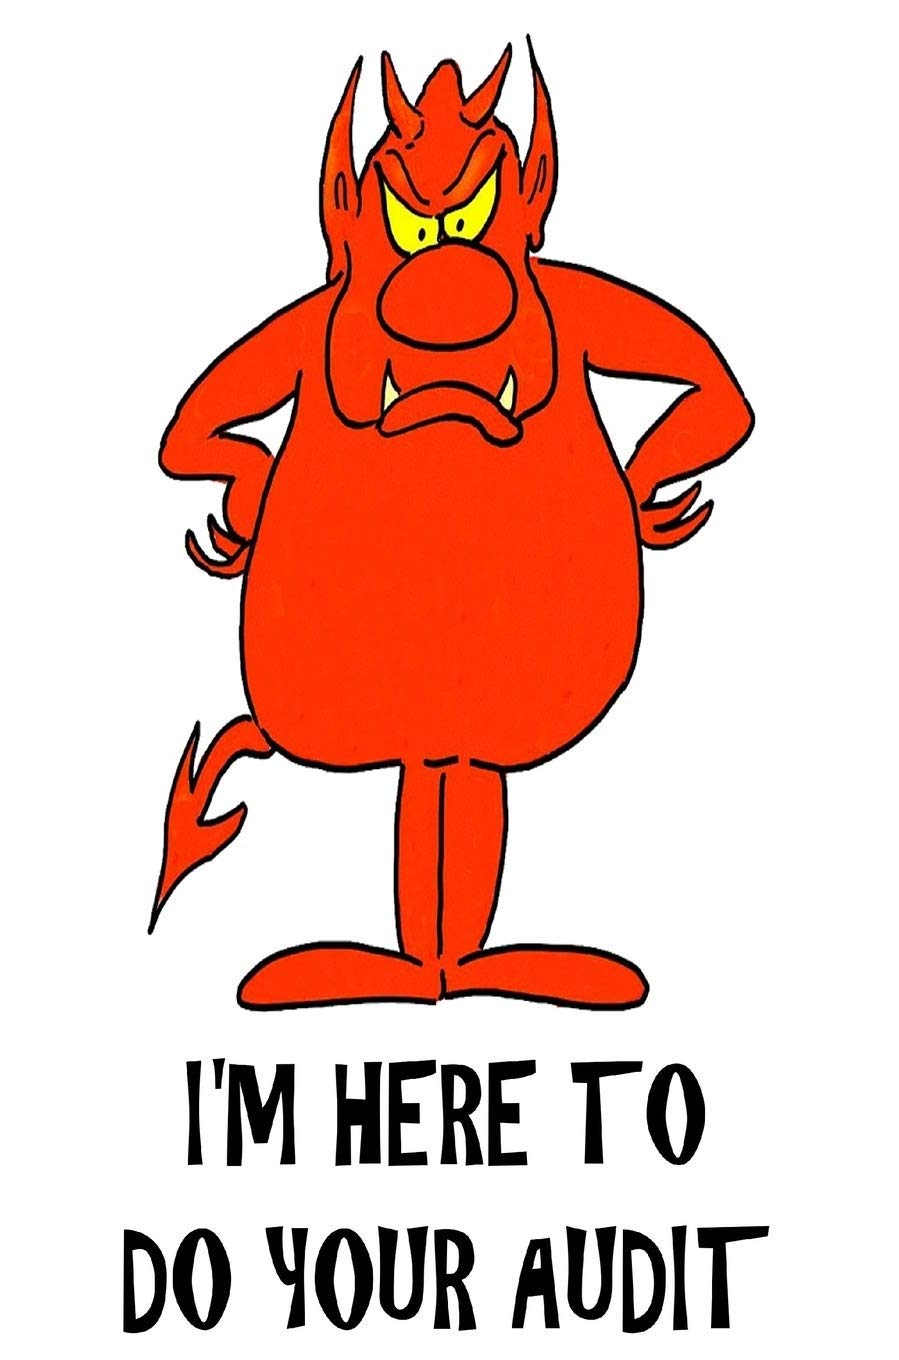
\includegraphics[max height = 0.3\textheight]{Images/devil.jpg}
    }{}

    \vspace*{.9em}
    Please mute yourselves!
    \end{center}


    \vfill
  \end{frame}
}

\AtBeginSubsection[]{
  \begin{frame}
    \vfill
    \centering
    \begin{beamercolorbox}[sep=8pt,center,shadow=true,rounded=true]{title}
    \usebeamerfont{title}\insertsectionhead\par%
    \usebeamerfont{subtitle}\insertsubsectionhead\par%
    \end{beamercolorbox}
    \ifthenelse{\equal{\subsecname}{Answers}} {
        \begin{center}
        Unmute yourselves!
        \end{center}
    }
    \vfill
  \end{frame}
}
\begin{document}

\title{Welcome to Saturday Night Trivia XVII!}
\date{}

\begin{frame}
\titlepage{}
\begin{center}

\includegraphics[max width=0.9\textwidth,
    max height=0.4\textheight]{Images/triviatitleframelogo.png}
\end{center}
\end{frame}

\begin{frame}
Welcome to the April edition of Saturday Night Trivia!
\pause
\begin{center}
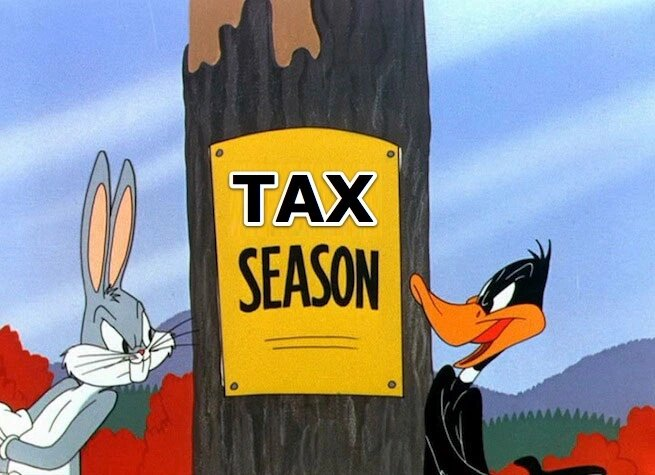
\includegraphics[max width=\textwidth,max height=\textheight]{Images/taxseason.jpg}
\end{center}
\end{frame}

\begingroup{}
\begingroup{}
\begin{frame}[t]{Categories}
This week, you'll be answering questions in the following categories:
\begin{enumerate}
\item Clothing Around the World
\item Dinosaurs
\item Political Slogans
\item I Love You, You're Perfect, Now be Past Perfect
\item Number One Songs
\item Things Dean Martin Never Said
\item Hey, look what I found(ed)!
\item Famous People of Medicine
\item Comedy Teams
\item Luxury Brands
\item Bonus Round
\end{enumerate}
\end{frame}
\endgroup{}

\begingroup{}
\begin{frame}
\vfill{}
\begin{beamercolorbox}[sep=8pt,center,shadow=true,rounded=true]{title}
\usebeamerfont{title}Good luck everyone! And have fun!
\end{beamercolorbox}
\vfill{}
\end{frame}
\endgroup{}
\def\thisSectionName{Clothing Around the World}
\section{Round 1}
\subsection*{Q1}
\begin{frame}[t]{Round 1 --- Clothing Around the World --- \mbox{Question 1}}
\vspace{-0.5em}
\begin{columns}[T,totalwidth=\linewidth]
\begin{column}{0.37\linewidth}
\begin{block}{Question}
What is the name of the  long, split tunic dress pictured here that is worn over trousers by Vietnamese women?
\end{block}
\end{column}
\begin{column}{0.62\linewidth}
\begin{center}
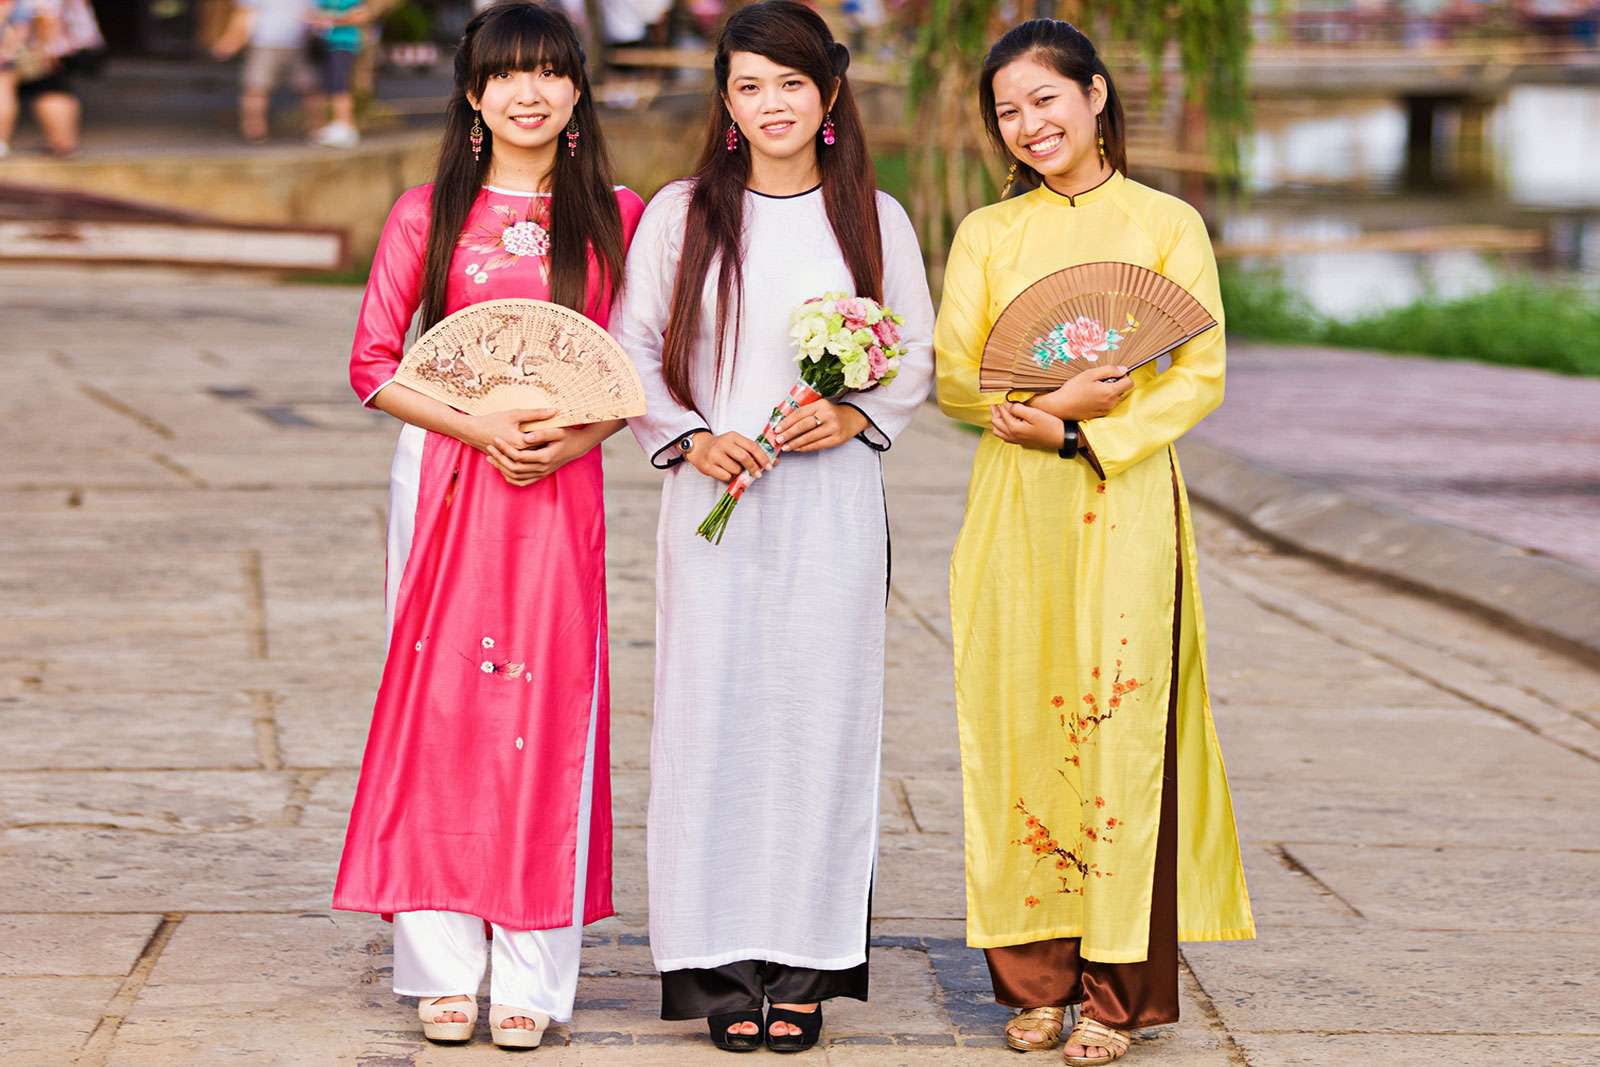
\includegraphics[max width=0.95\textwidth,max height=0.7\textheight]{{Images/aodai}.jpg}
\end{center}
\end{column}
\end{columns}
\end{frame}
\subsection*{Q2}
\begin{frame}[t]{Round 1 --- Clothing Around the World --- \mbox{Question 2}}
\vspace{-0.5em}
\begin{block}{Question}
What is the name of the hat worn in Morocco that shares its name with a Moroccan city?
\end{block}
\end{frame}
\subsection*{Q3}
\begin{frame}[t]{Round 1 --- Clothing Around the World --- \mbox{Question 3}}
\vspace{-0.5em}
\begin{columns}[T,totalwidth=\linewidth]
\begin{column}{0.37\linewidth}
\begin{block}{Question}
What is the name of the traditional German pants shown here, whose name translates literally as ``leather trousers''?
\end{block}
\end{column}
\begin{column}{0.62\linewidth}
\begin{center}
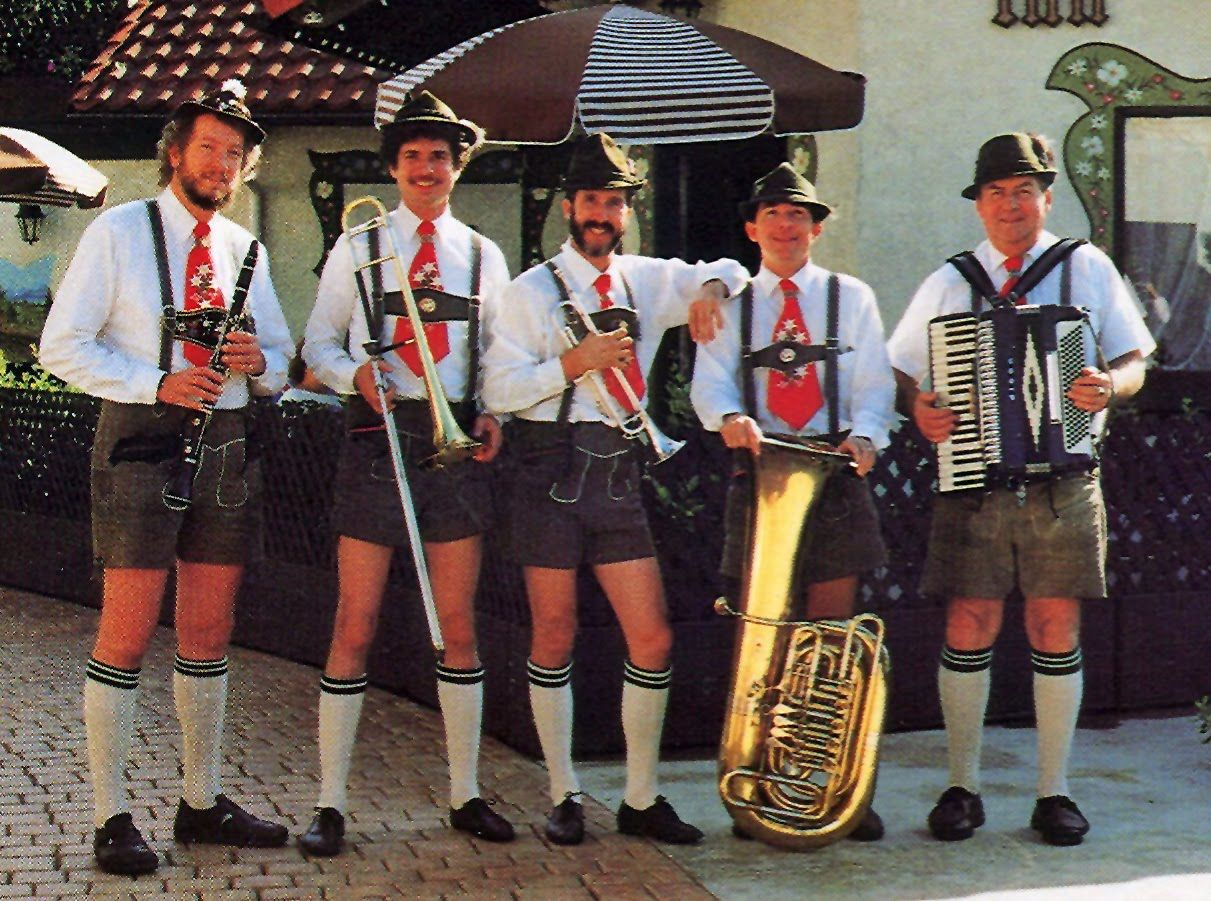
\includegraphics[max width=0.95\textwidth,max height=0.7\textheight]{{Images/lederhosen}.jpg}
\end{center}
\end{column}
\end{columns}
\end{frame}
\subsection*{Q4}
\begin{frame}[t]{Round 1 --- Clothing Around the World --- \mbox{Question 4}}
\vspace{-0.5em}
\begin{columns}[T,totalwidth=\linewidth]
\begin{column}{0.37\linewidth}
\begin{block}{Question}
What is the name of the furry Russian hat with ear flaps that can be tied under the chin (or pulled up and tied at the top of the hat when the wearer is in Moscow instead of Siberia)?
\end{block}
\end{column}
\begin{column}{0.62\linewidth}
\begin{center}
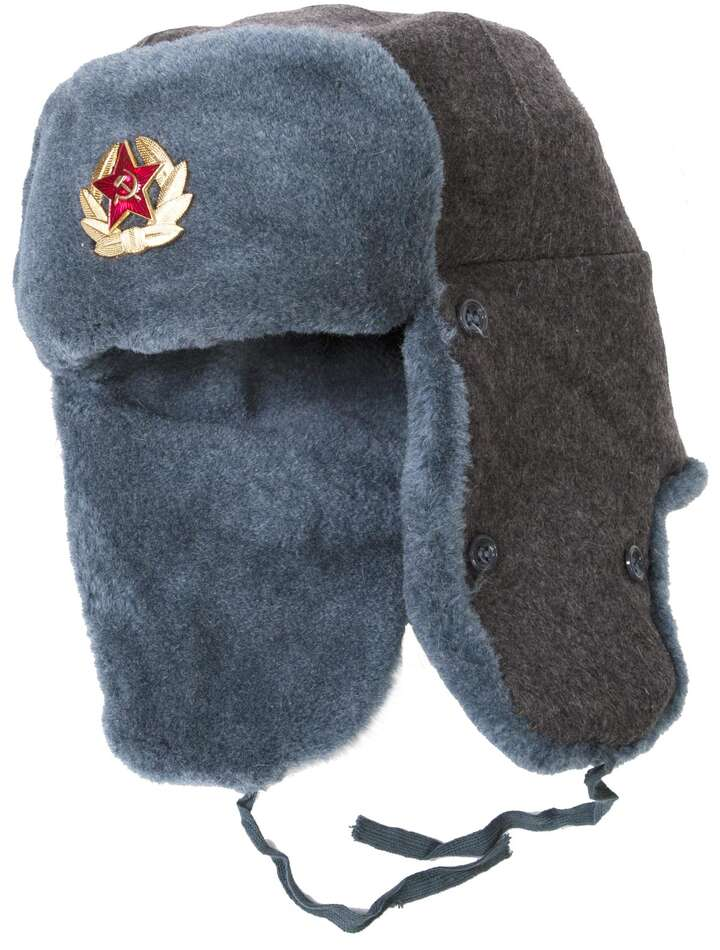
\includegraphics[max width=0.95\textwidth,max height=0.7\textheight]{{Images/ushanka}.jpeg}
\end{center}
\end{column}
\end{columns}
\end{frame}
\subsection*{Q5}
\begin{frame}[t]{Round 1 --- Clothing Around the World --- \mbox{Question 5}}
\vspace{-0.5em}
\begin{columns}[T,totalwidth=\linewidth]
\begin{column}{0.37\linewidth}
\begin{block}{Question}
Which country do the socks shown here, intended to be worn with flip flop-style footwear, come from?
\end{block}
\end{column}
\begin{column}{0.62\linewidth}
\begin{center}
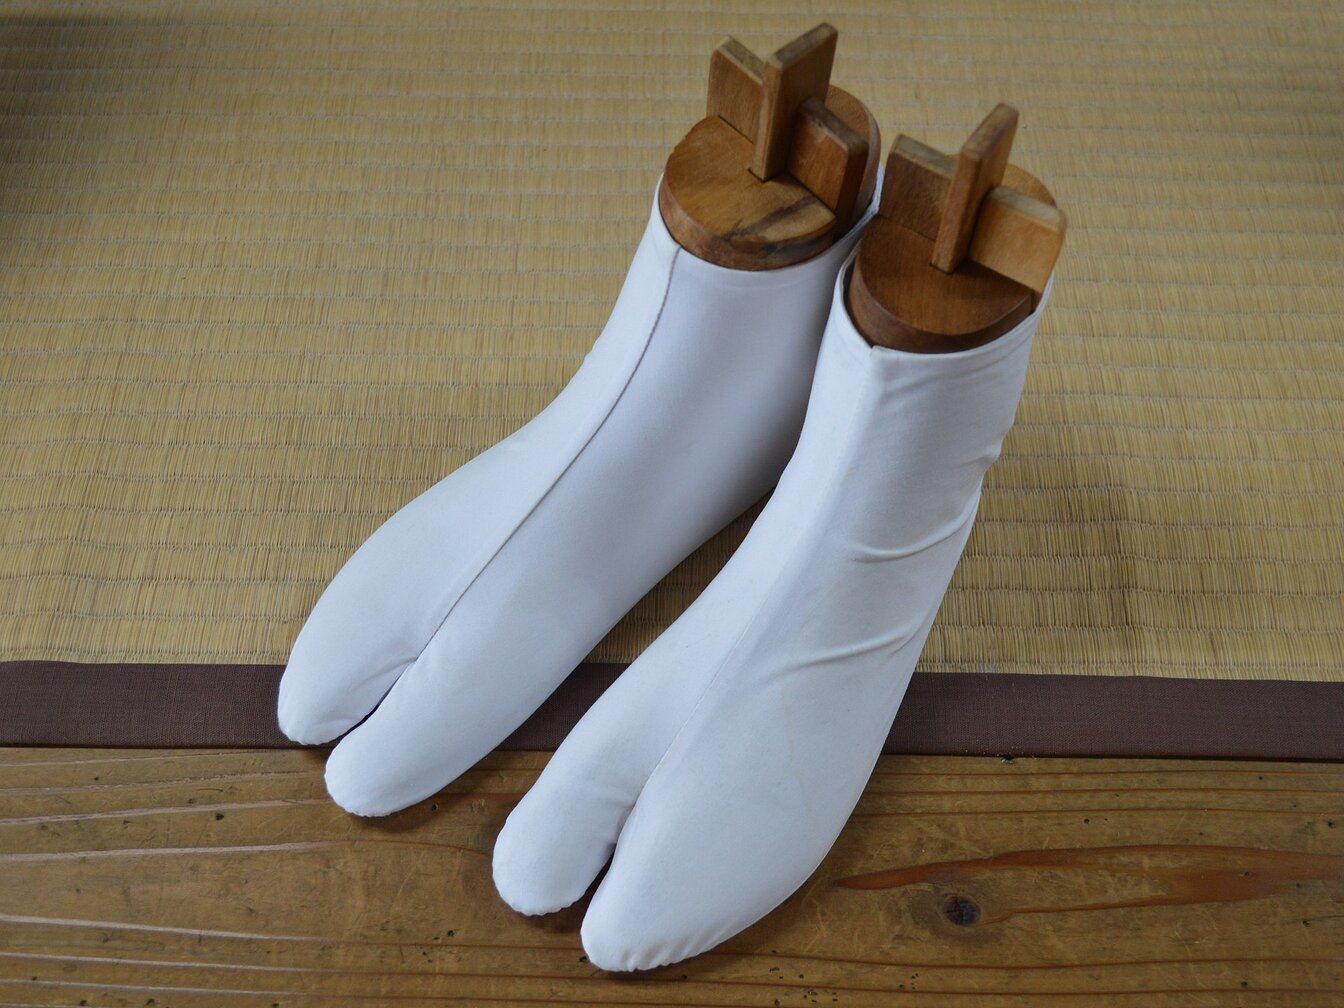
\includegraphics[max width=0.95\textwidth,max height=0.7\textheight]{{Images/tabi}.jpg}
\end{center}
\end{column}
\end{columns}
\end{frame}
\subsection*{Q6}
\begin{frame}[t]{Round 1 --- Clothing Around the World --- \mbox{Question 6}}
\vspace{-0.5em}
\begin{columns}[T,totalwidth=\linewidth]
\begin{column}{0.37\linewidth}
\begin{block}{Question}
What is the name of the garment shown here, which is worn in Western Africa?
\end{block}
\end{column}
\begin{column}{0.62\linewidth}
\begin{center}
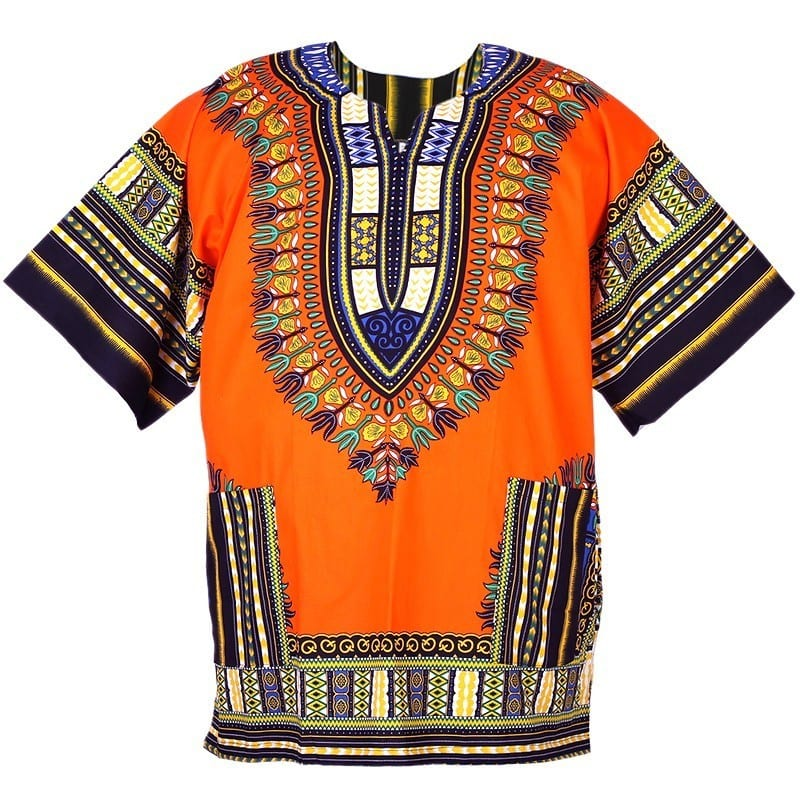
\includegraphics[max width=0.95\textwidth,max height=0.7\textheight]{{Images/dashiki}.jpg}
\end{center}
\end{column}
\end{columns}
\end{frame}
\subsection*{Q7}
\begin{frame}[t]{Round 1 --- Clothing Around the World --- \mbox{Question 7}}
\vspace{-0.5em}
\begin{columns}[T,totalwidth=\linewidth]
\begin{column}{0.37\linewidth}
\begin{block}{Question}
What is the name of the traditional Scottish hat shown here that is frequently worn by Scottish military officers?
\end{block}
\end{column}
\begin{column}{0.62\linewidth}
\begin{center}
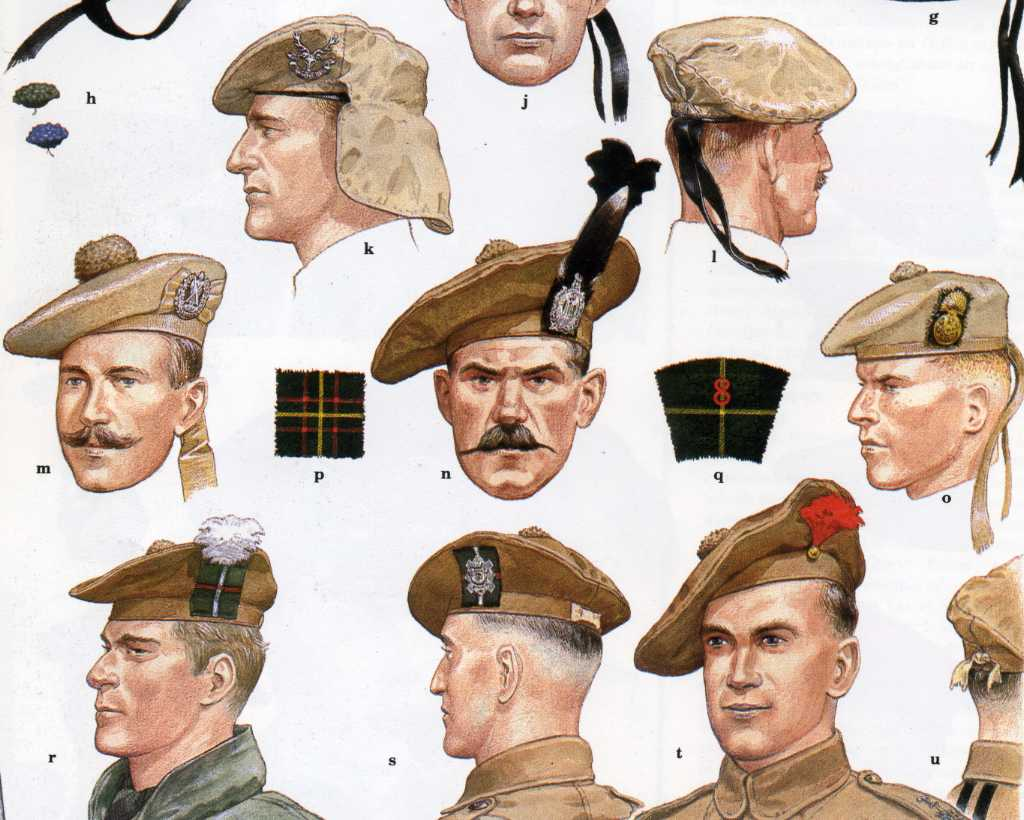
\includegraphics[max width=0.95\textwidth,max height=0.7\textheight]{{Images/tamoshanter}.jpeg}
\end{center}
\end{column}
\end{columns}
\end{frame}
\subsection*{Q8}
\begin{frame}[t]{Round 1 --- Clothing Around the World --- \mbox{Question 8}}
\vspace{-0.5em}
\begin{columns}[T,totalwidth=\linewidth]
\begin{column}{0.37\linewidth}
\begin{block}{Question}
What is the name of the shoe pictured here, which is worn in the area of Italy southwest of Rome known as the Ciociaria?
\end{block}
\end{column}
\begin{column}{0.62\linewidth}
\begin{center}
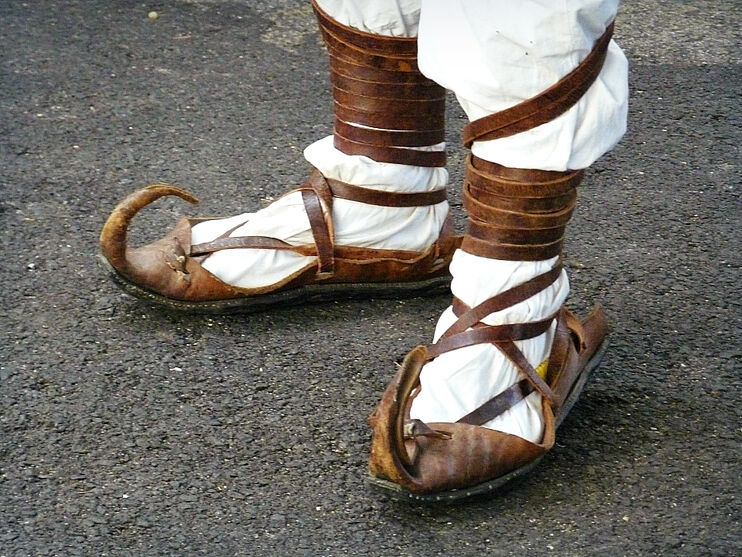
\includegraphics[max width=0.95\textwidth,max height=0.7\textheight]{{Images/italianshoe}.jpg}
\end{center}
\end{column}
\end{columns}
\end{frame}
\subsection*{Q9}
\begin{frame}[t]{Round 1 --- Clothing Around the World --- \mbox{Question 9}}
\vspace{-0.5em}
\begin{columns}[T,totalwidth=\linewidth]
\begin{column}{0.37\linewidth}
\begin{block}{Question}
What is the name of the lower-body garment shown here, which is created from a length of fabric wrapped around the waist and is ubiquitous in Southern and Southeast Asia?
\end{block}
\end{column}
\begin{column}{0.62\linewidth}
\begin{center}
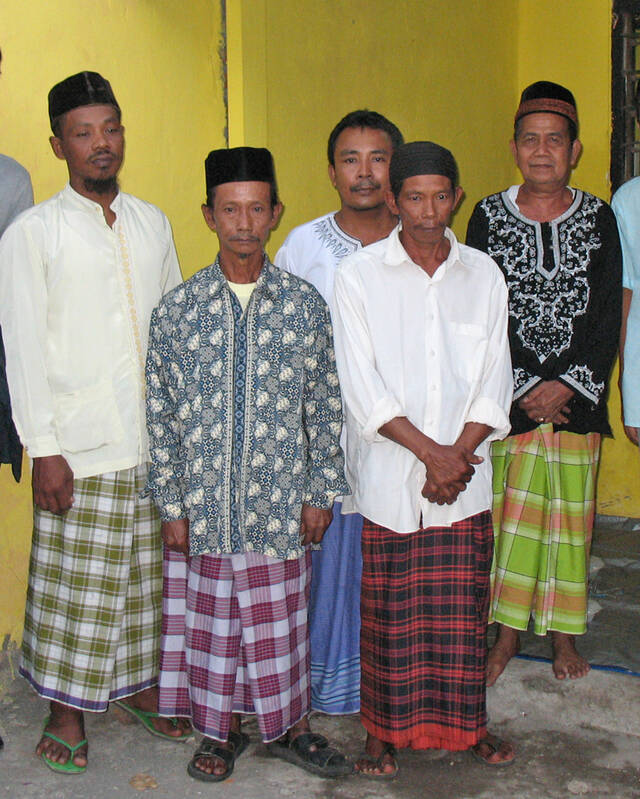
\includegraphics[max width=0.95\textwidth,max height=0.7\textheight]{{Images/sarong}.jpg}
\end{center}
\end{column}
\end{columns}
\end{frame}
\subsection*{Q10}
\begin{frame}[t]{Round 1 --- Clothing Around the World --- \mbox{Question 10}}
\vspace{-0.5em}
\begin{columns}[T,totalwidth=\linewidth]
\begin{column}{0.37\linewidth}
\begin{block}{Question}
What is the name of the long coats pictured here (from the movies \emph{Pale Rider} and \emph{Once Upon a Time in the West}), which were often worn by cowboys and gunslingers?
\end{block}
\end{column}
\begin{column}{0.62\linewidth}
\begin{center}
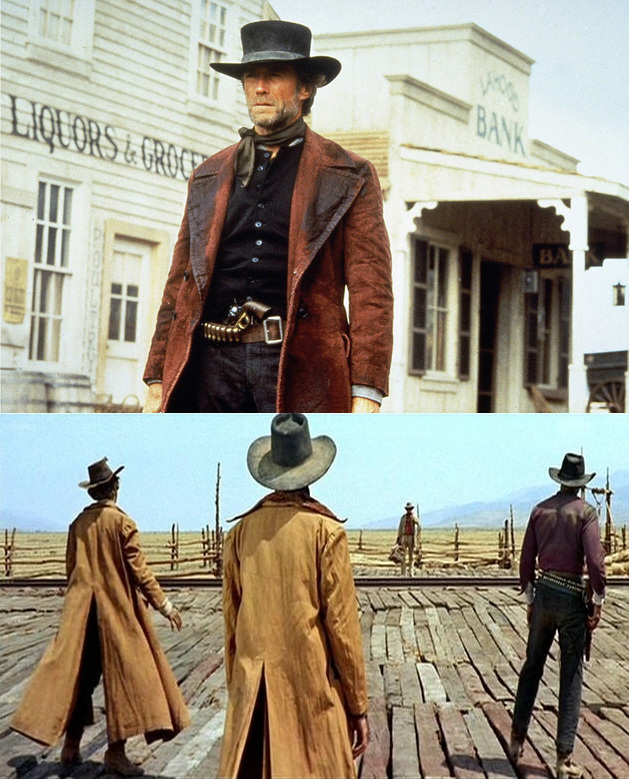
\includegraphics[max width=0.95\textwidth,max height=0.7\textheight]{{Images/duster}.jpg}
\end{center}
\end{column}
\end{columns}
\end{frame}
\subsection{Answers}
\begin{frame}[t]{Round 1 --- Clothing Around the World --- \mbox{Answer 1}}
\vspace{-0.5em}
\begin{columns}[T,totalwidth=\linewidth]
    \begin{column}{0.6\linewidth}
    \begin{block}{Question}
    What is the name of the  long, split tunic dress pictured here that is worn over trousers by Vietnamese women?
    \end{block}
    \end{column}
    \begin{column}{0.38\linewidth}
    \begin{center}
    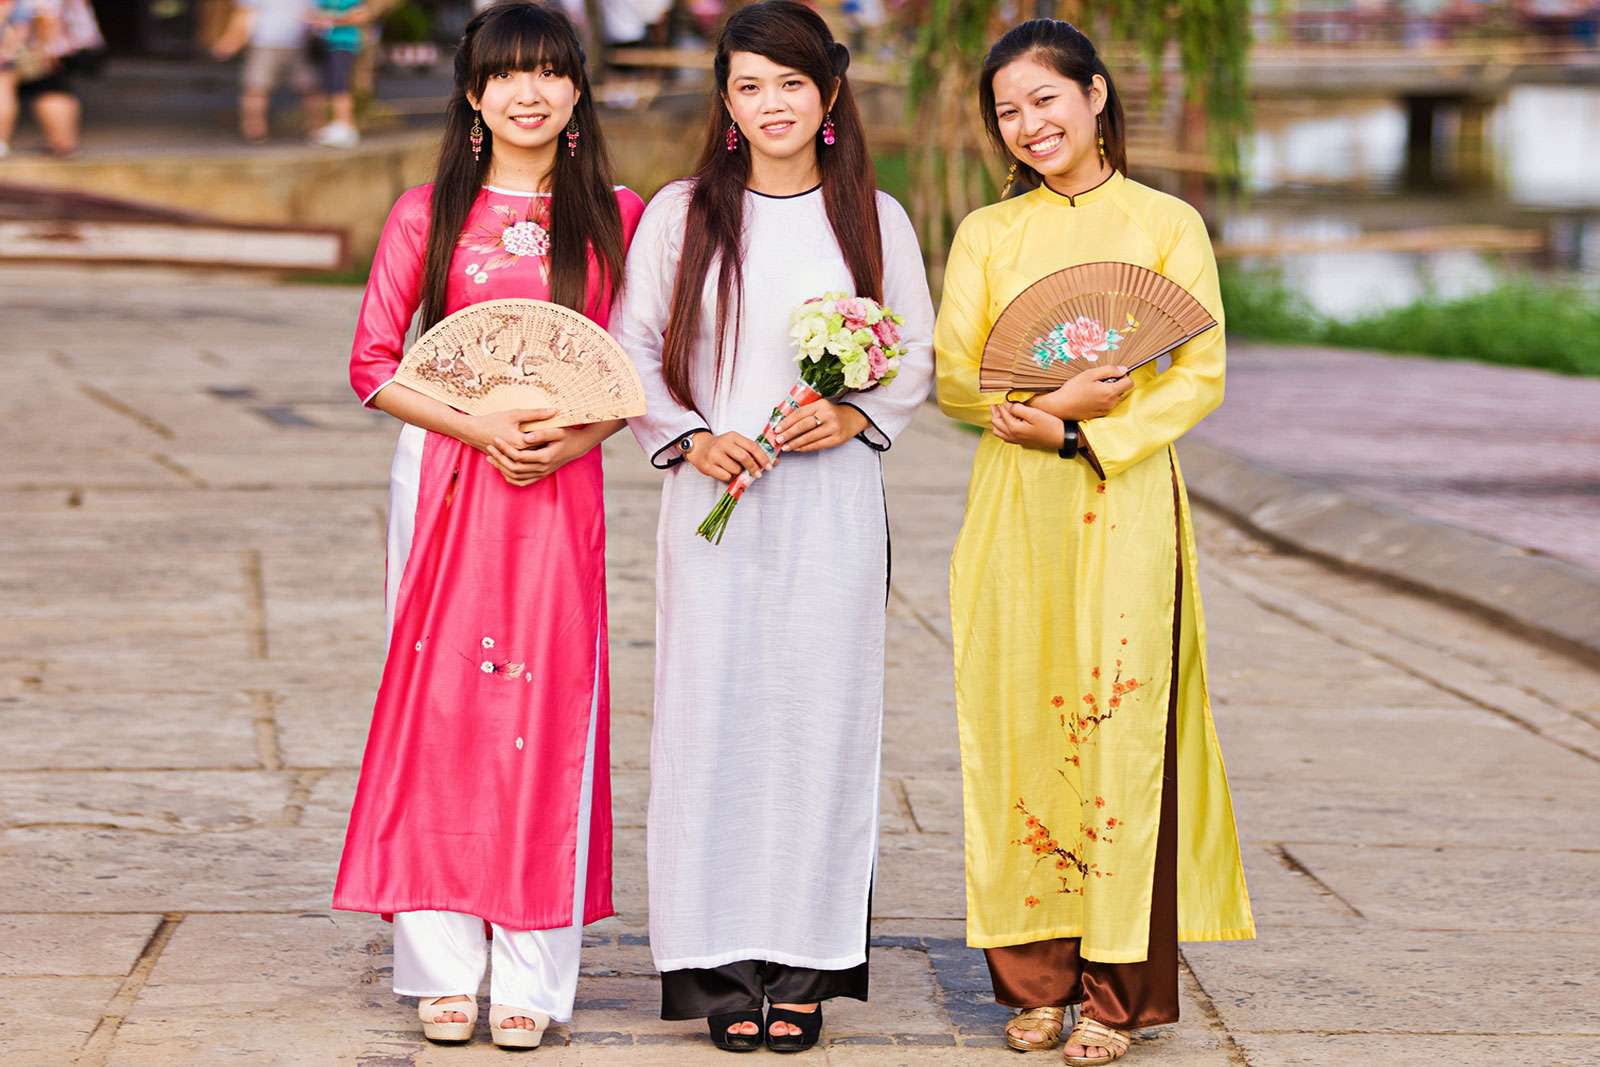
\includegraphics[max width=0.95\textwidth,
        max height=3in]{{Images/aodai}.jpg}
    \end{center}
    \end{column}
\end{columns}

\visible<2->{
    \begin{block}{Answer}
    {\'A}o d{\`a}i (without the tonal marks is fine).  Any phonetic equivalent of ``ow yie'' or ``ow zie'' is also acceptable.
    \end{block}
}
\end{frame}
\begin{frame}[t]{Round 1 --- Clothing Around the World --- \mbox{Answer 2}}
\vspace{-0.5em}
\begin{block}{Question}
What is the name of the hat worn in Morocco that shares its name with a Moroccan city?
\end{block}

\visible<2->{
    \begin{columns}[T,totalwidth=\linewidth]
    \begin{column}{0.32\linewidth}
    \begin{block}{Answer}
    Fez
    \end{block}
    \end{column}
    \begin{column}{0.65\linewidth}
    \begin{center}
    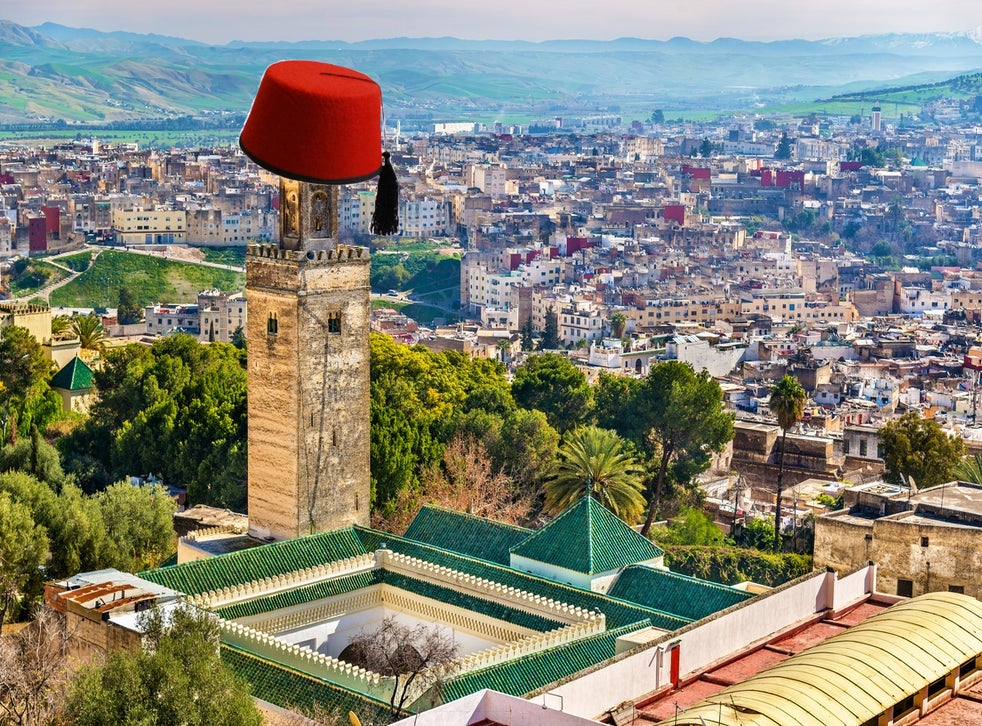
\includegraphics[max height=.45\textheight,
        max width=0.95\textwidth]{{Images/fez}.jpg}
    \end{center}
    \end{column}
    \end{columns}
}
\end{frame}
\begin{frame}[t]{Round 1 --- Clothing Around the World --- \mbox{Answer 3}}
\vspace{-0.5em}
\begin{columns}[T,totalwidth=\linewidth]
\begin{column}{0.32\linewidth}
\begin{block}{Question}
What is the name of the traditional German pants shown here, whose name translates literally as ``leather trousers''?
\end{block}
\visible<2->{
    \begin{block}{Answer}
    Lederhosen
    \end{block}
}
\end{column}
\begin{column}{0.65\linewidth}
\begin{center}
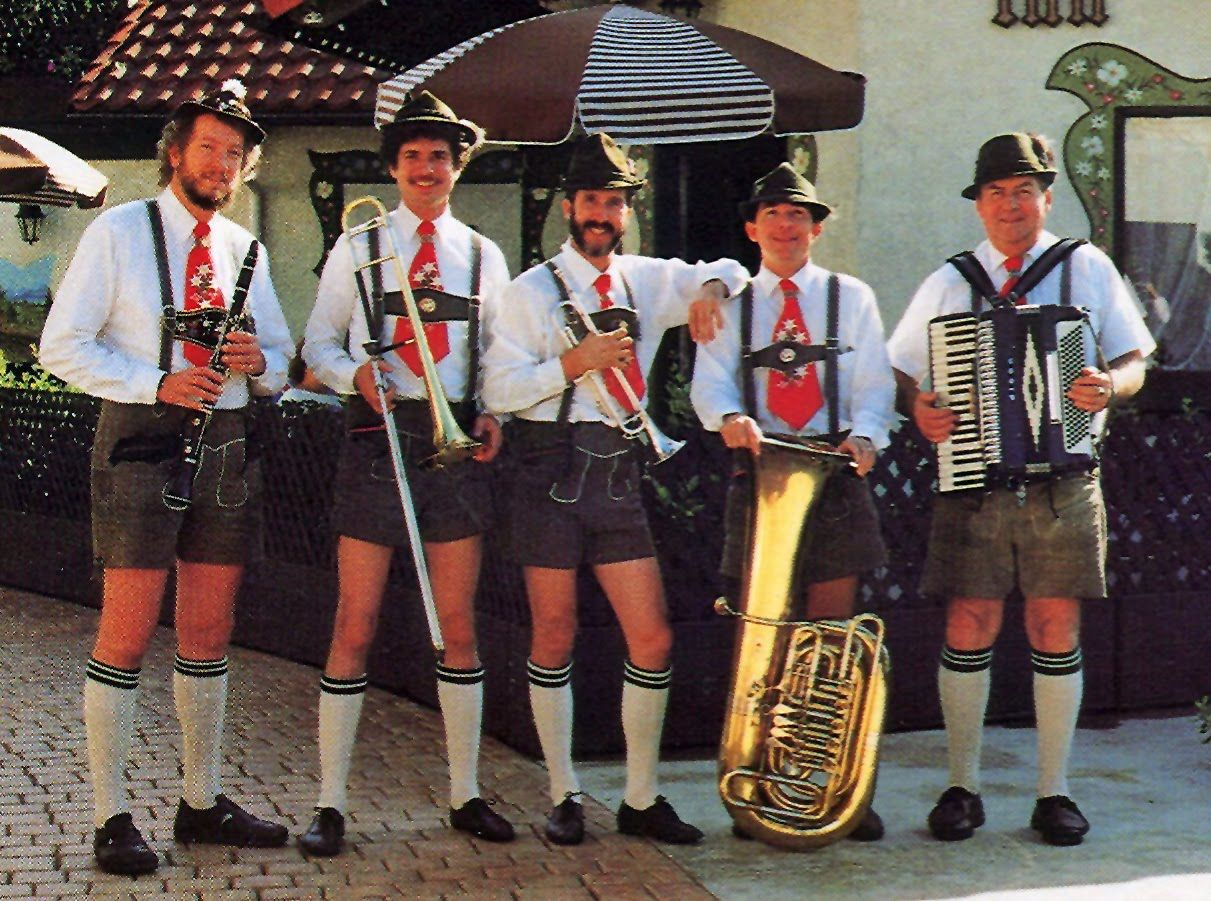
\includegraphics[max width=0.95\textwidth,max height=0.7\textheight]{{Images/lederhosen}.jpg}
\end{center}
\end{column}
\end{columns}
\end{frame}
\begin{frame}[t]{Round 1 --- Clothing Around the World --- \mbox{Answer 4}}
\vspace{-0.5em}
\begin{columns}[T,totalwidth=\linewidth]
    \begin{column}{0.6\linewidth}
    \begin{block}{Question}
    What is the name of the furry Russian hat with ear flaps that can be tied under the chin (or pulled up and tied at the top of the hat when the wearer is in Moscow instead of Siberia)?
    \end{block}
    \end{column}
    \begin{column}{0.38\linewidth}
    \begin{center}
    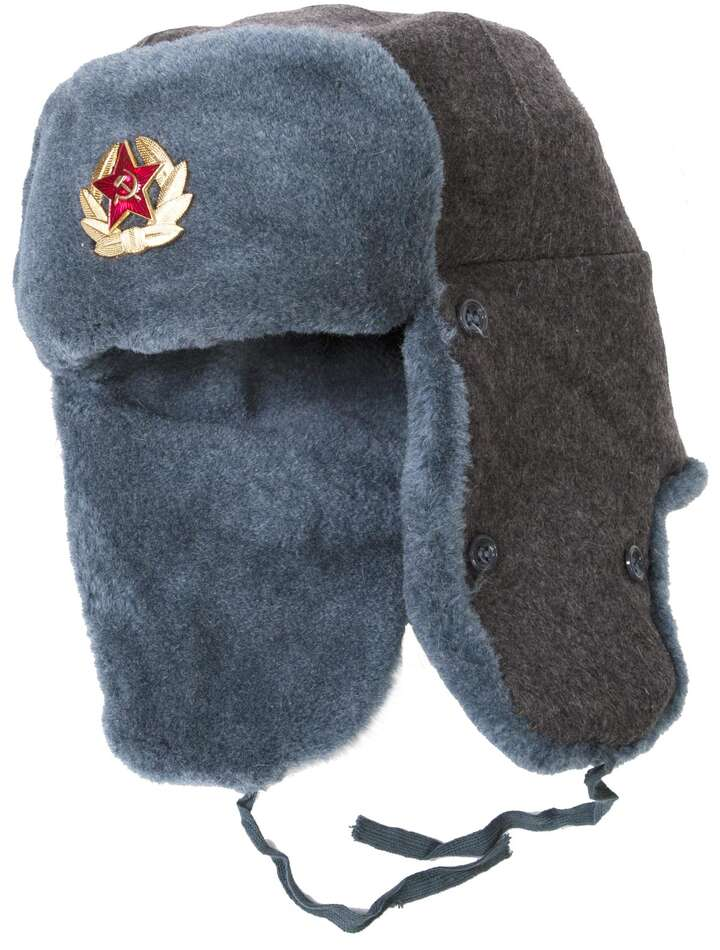
\includegraphics[max width=0.95\textwidth,
        max height=3in]{{Images/ushanka}.jpeg}
    \end{center}
    \end{column}
\end{columns}

\visible<2->{
    \begin{block}{Answer}
    Ushanka (literally ``ear flap hat'')
    \end{block}
}
\end{frame}
\begin{frame}[t]{Round 1 --- Clothing Around the World --- \mbox{Answer 5}}
\vspace{-0.5em}
\begin{columns}[T,totalwidth=\linewidth]
\begin{column}{0.32\linewidth}
\begin{block}{Question}
Which country do the socks shown here, intended to be worn with flip flop-style footwear, come from?
\end{block}
\visible<2->{
    \begin{block}{Answer}
    Japan
    \end{block}
}
\end{column}
\begin{column}{0.65\linewidth}
\begin{center}
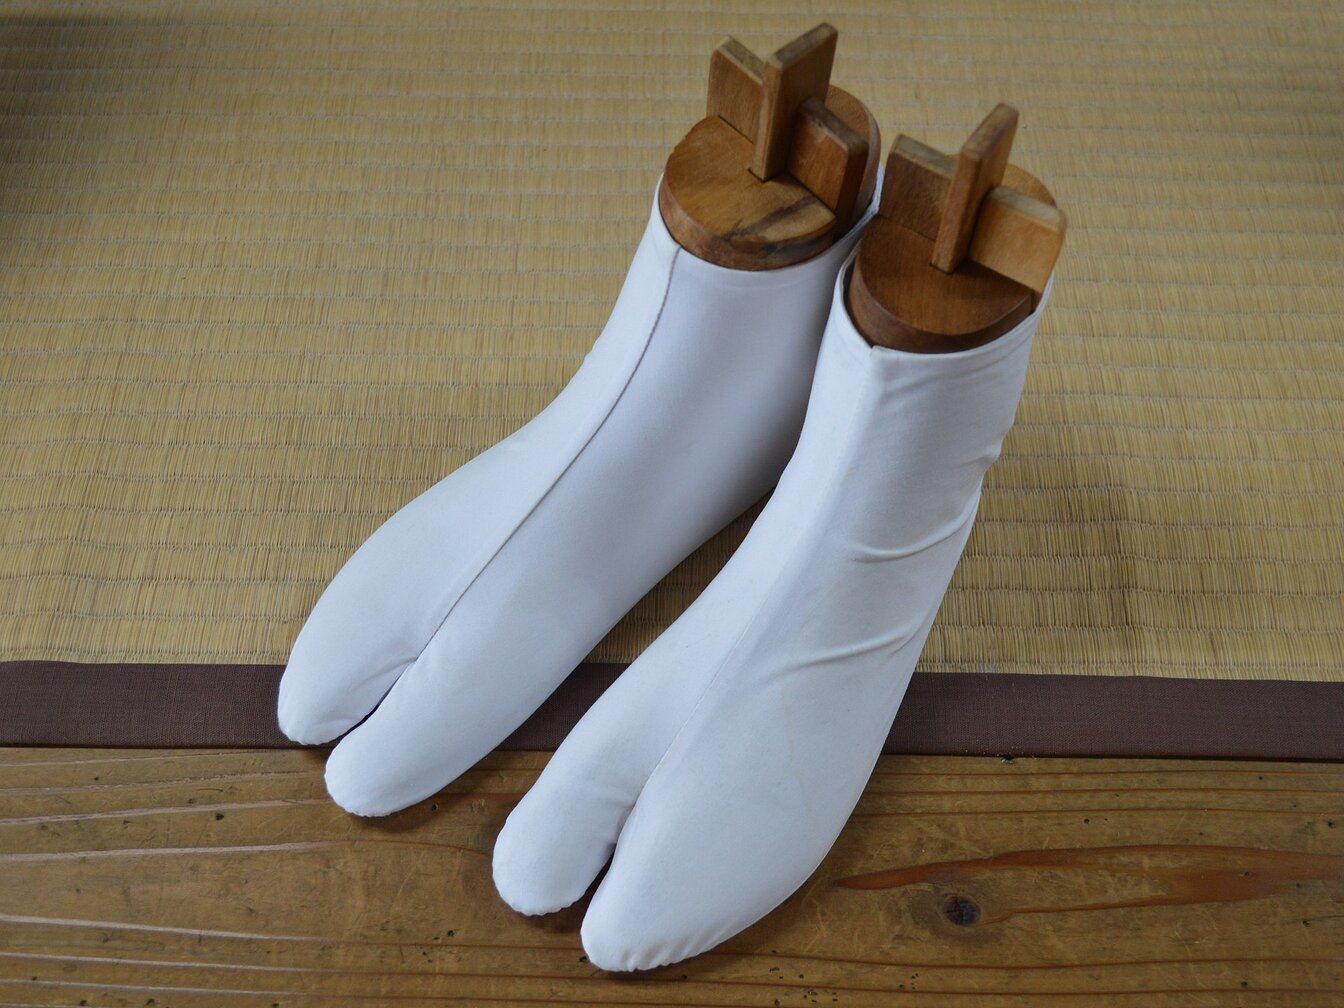
\includegraphics[max width=0.95\textwidth,max height=0.7\textheight]{{Images/tabi}.jpg}
\end{center}
\end{column}
\end{columns}
\end{frame}
\begin{frame}[t]{Round 1 --- Clothing Around the World --- \mbox{Answer 6}}
\vspace{-0.5em}
\begin{columns}[T,totalwidth=\linewidth]
\begin{column}{0.32\linewidth}
\begin{block}{Question}
What is the name of the garment shown here, which is worn in Western Africa?
\end{block}
\visible<2->{
    \begin{block}{Answer}
    Dashiki
    \end{block}
}
\end{column}
\begin{column}{0.65\linewidth}
\begin{center}
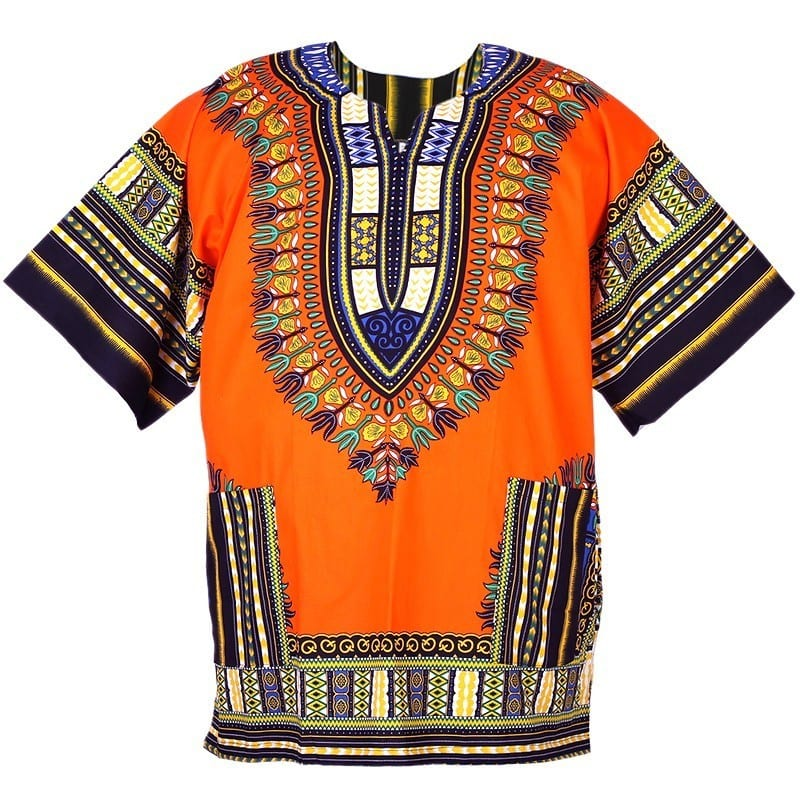
\includegraphics[max width=0.95\textwidth,max height=0.7\textheight]{{Images/dashiki}.jpg}
\end{center}
\end{column}
\end{columns}
\end{frame}
\begin{frame}[t]{Round 1 --- Clothing Around the World --- \mbox{Answer 7}}
\vspace{-0.5em}
\begin{columns}[T,totalwidth=\linewidth]
\begin{column}{0.32\linewidth}
\begin{block}{Question}
What is the name of the traditional Scottish hat shown here that is frequently worn by Scottish military officers?
\end{block}
\visible<2->{
    \begin{block}{Answer}
    Tam o' shanter / Tammie
    \end{block}
}
\end{column}
\begin{column}{0.65\linewidth}
\begin{center}
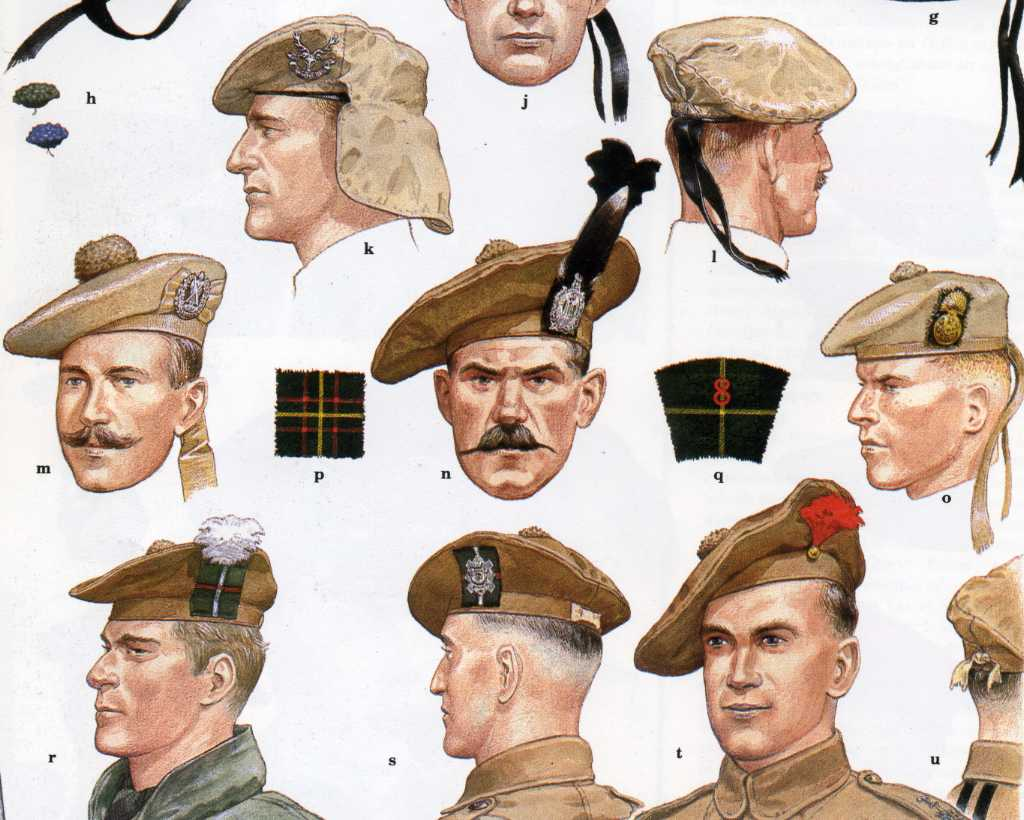
\includegraphics[max width=0.95\textwidth,max height=0.7\textheight]{{Images/tamoshanter}.jpeg}
\end{center}
\end{column}
\end{columns}
\end{frame}
\begin{frame}[t]{Round 1 --- Clothing Around the World --- \mbox{Answer 8}}
\vspace{-0.5em}
\begin{columns}[T,totalwidth=\linewidth]
    \begin{column}{0.6\linewidth}
    \begin{block}{Question}
    What is the name of the shoe pictured here, which is worn in the area of Italy southwest of Rome known as the Ciociaria?
    \end{block}
    \end{column}
    \begin{column}{0.38\linewidth}
    \begin{center}
    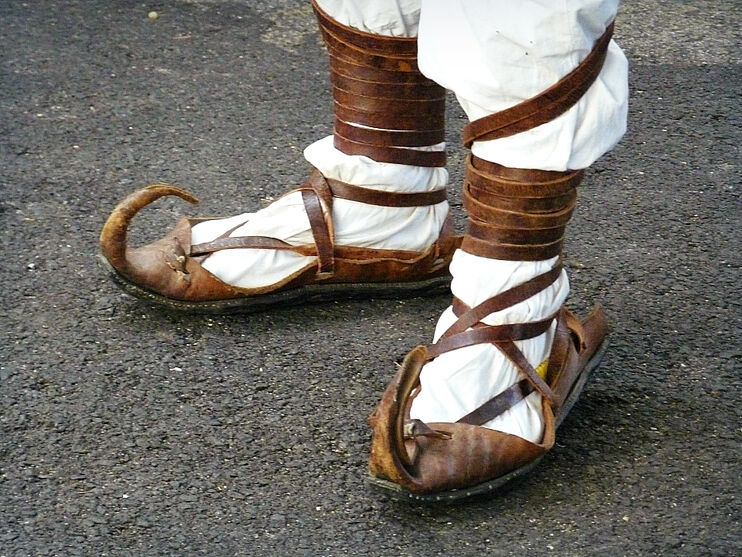
\includegraphics[max width=0.95\textwidth,
        max height=3in]{{Images/italianshoe}.jpg}
    \end{center}
    \end{column}
\end{columns}

\visible<2->{
    \begin{block}{Answer}
    Ciocia (plural ciocie).  (The Ciociaria is the region where people traditionally wore ciocie.) 
    \end{block}
}
\end{frame}
\begin{frame}[t]{Round 1 --- Clothing Around the World --- \mbox{Answer 9}}
\vspace{-0.5em}
\begin{columns}[T,totalwidth=\linewidth]
    \begin{column}{0.4\linewidth}
    \begin{block}{Question}
    What is the name of the lower-body garment shown here, which is created from a length of fabric wrapped around the waist and is ubiquitous in Southern and Southeast Asia?
    \end{block}
    \end{column}
    \begin{column}{0.58\linewidth}
    \begin{center}
    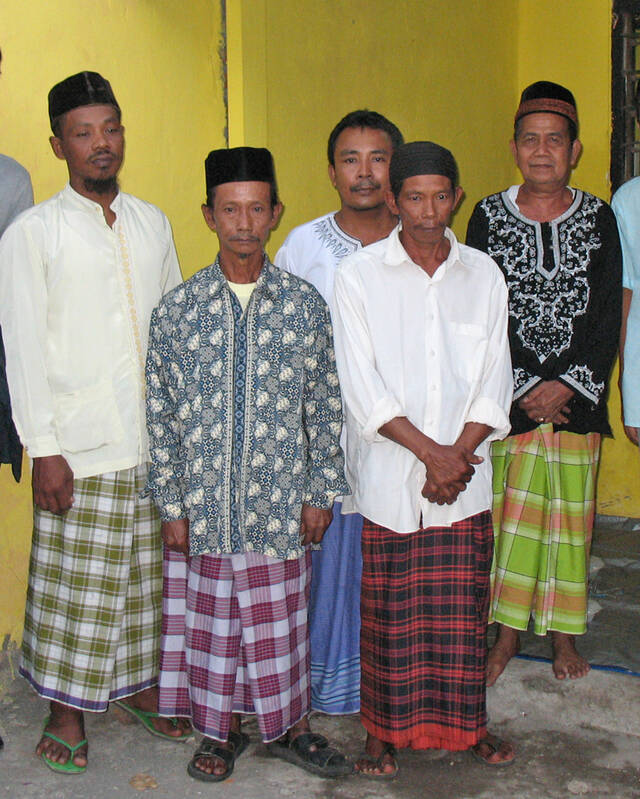
\includegraphics[max width=0.95\textwidth,
        max height=2.2in]{{Images/sarong}.jpg}
    \end{center}
    \end{column}
\end{columns}

\visible<2->{
    \begin{block}{Answer}
    Sarong / sarung
    \end{block}
}
\end{frame}
\begin{frame}[t]{Round 1 --- Clothing Around the World --- \mbox{Answer 10}}
\vspace{-0.5em}
\begin{columns}[T,totalwidth=\linewidth]
\begin{column}{0.32\linewidth}
\begin{block}{Question}
What is the name of the long coats pictured here (from the movies \emph{Pale Rider} and \emph{Once Upon a Time in the West}), which were often worn by cowboys and gunslingers?
\end{block}
\visible<2->{
    \begin{block}{Answer}
    Dusters
    \end{block}
}
\end{column}
\begin{column}{0.65\linewidth}
\begin{center}
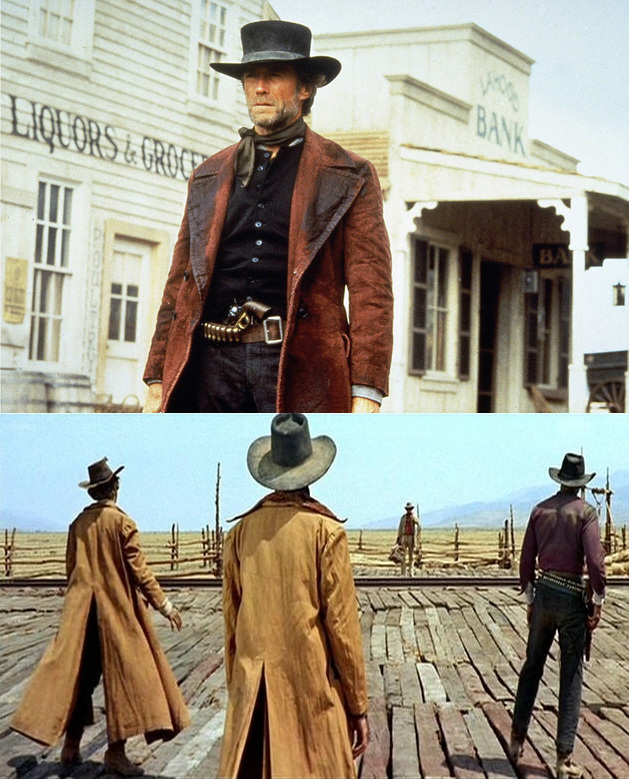
\includegraphics[max width=0.95\textwidth,max height=0.7\textheight]{{Images/duster}.jpg}
\end{center}
\end{column}
\end{columns}
\end{frame}
\def\thisSectionName{Dinosaurs}
\section{Round 2}
\subsection*{Q1}
\begin{frame}[t]{Round 2 --- Dinosaurs --- \mbox{Question 1}}
\vspace{-0.5em}
\begin{block}{Question}
The Modern Latin roots of the word ``dinosaur'' --- ``dino'' + ``saur'' --- are usually translated into what English words?
\end{block}
\end{frame}
\subsection*{Q2}
\begin{frame}[t]{Round 2 --- Dinosaurs --- \mbox{Question 2}}
\vspace{-0.5em}
\begin{block}{Question}
Which two people were the executive producers of the 1988 animated children's film about a group of dinosaurs, \emph{The Land Before Time}?
\end{block}
\end{frame}
\subsection*{Q3}
\begin{frame}[t]{Round 2 --- Dinosaurs --- \mbox{Question 3}}
\vspace{-0.5em}
\begin{block}{Question}
Which city does the NBA team The Raptors play in?
\end{block}
\end{frame}
\subsection*{Q4}
\begin{frame}[t]{Round 2 --- Dinosaurs --- \mbox{Question 4}}
\vspace{-0.5em}
\begin{block}{Question}
To within 5 million years, how many years ago were the (non-avian) dinosaurs wiped out by an asteroid?
\end{block}
\end{frame}
\subsection*{Q5}
\begin{frame}[t]{Round 2 --- Dinosaurs --- \mbox{Question 5}}
\vspace{-0.5em}
\begin{block}{Question}
Which large oil and gas company has a sauropod in its logo?
\end{block}
\end{frame}
\subsection*{Q6}
\begin{frame}[t]{Round 2 --- Dinosaurs --- \mbox{Question 6}}
\vspace{-0.5em}
\begin{columns}[T,totalwidth=\linewidth]
\begin{column}{0.37\linewidth}
\begin{block}{Question}
Pictured here is an artist's rendition of which species of bird-like dinosaur that is generally believed to be the ancestor of all modern birds?
\end{block}
\end{column}
\begin{column}{0.62\linewidth}
\begin{center}
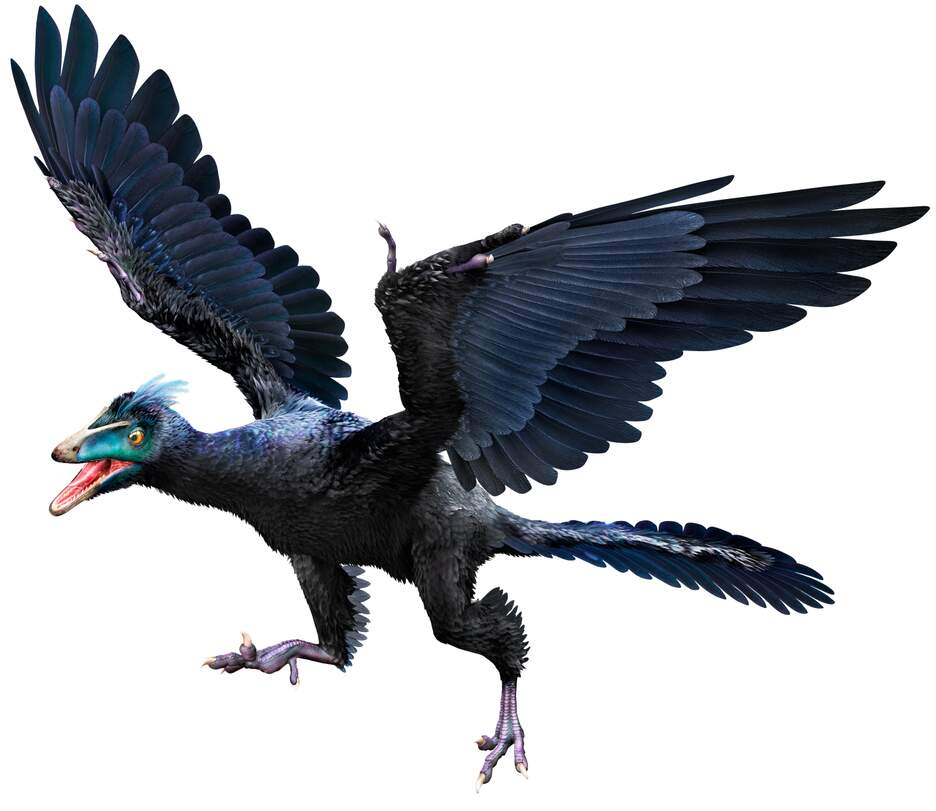
\includegraphics[max width=0.95\textwidth,max height=0.7\textheight]{{Images/archaeopteryx}.jpg}
\end{center}
\end{column}
\end{columns}
\end{frame}
\subsection*{Q7}
\begin{frame}[t]{Round 2 --- Dinosaurs --- \mbox{Question 7}}
\vspace{-0.5em}
\begin{block}{Question}
In what year was \emph{Jurassic Park} released?
\end{block}
\end{frame}
\subsection*{Q8}
\begin{frame}[t]{Round 2 --- Dinosaurs --- \mbox{Question 8}}
\vspace{-0.5em}
\begin{block}{Question}
On \emph{Pee-wee's Playhouse}, what was the name of Pee-wee Herman's dinosaur friend?
\end{block}
\end{frame}
\subsection*{Q9}
\begin{frame}[t]{Round 2 --- Dinosaurs --- \mbox{Question 9}}
\vspace{-0.5em}
\begin{columns}[T,totalwidth=\linewidth]
\begin{column}{0.37\linewidth}
\begin{block}{Question}
The skeleton of what kind of dinosaur is pictured here?
\end{block}
\end{column}
\begin{column}{0.62\linewidth}
\begin{center}
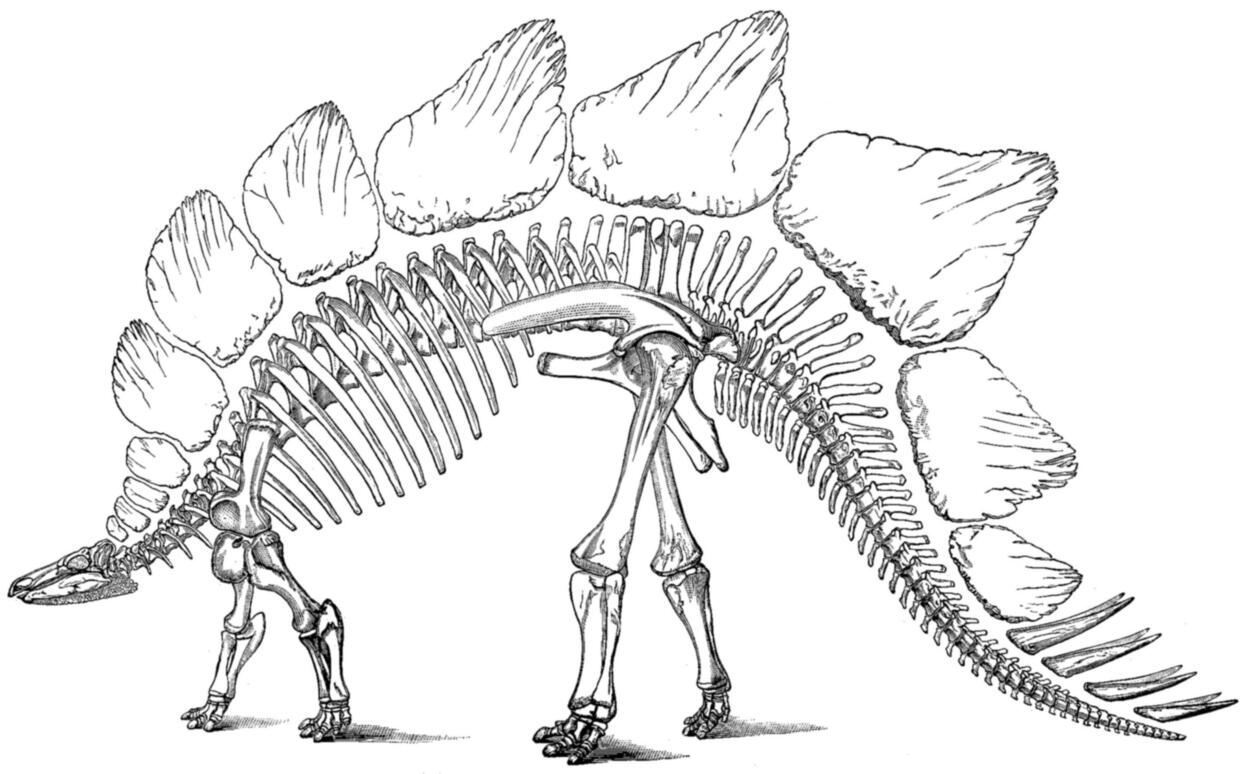
\includegraphics[max width=0.95\textwidth,max height=0.7\textheight]{{Images/stego}.jpg}
\end{center}
\end{column}
\end{columns}
\end{frame}
\subsection*{Q10}
\begin{frame}[t]{Round 2 --- Dinosaurs --- \mbox{Question 10}}
\vspace{-0.5em}
\begin{block}{Question}
What is the name of the period of intense, competitive hunting for dinosaur fossils that took place in the U.S. near the end of the 19\textsuperscript{th} Century?
\end{block}
\end{frame}
\subsection{Answers}
\begin{frame}[t]{Round 2 --- Dinosaurs --- \mbox{Answer 1}}
\vspace{-0.5em}
\begin{block}{Question}
The Modern Latin roots of the word ``dinosaur'' --- ``dino'' + ``saur'' --- are usually translated into what English words?
\end{block}

\visible<2->{
    \begin{columns}[T,totalwidth=\linewidth]
    \begin{column}{0.32\linewidth}
    \begin{block}{Answer}
    Terrible lizard / terrible reptile
    \end{block}
    \end{column}
    \begin{column}{0.65\linewidth}
    \begin{center}
    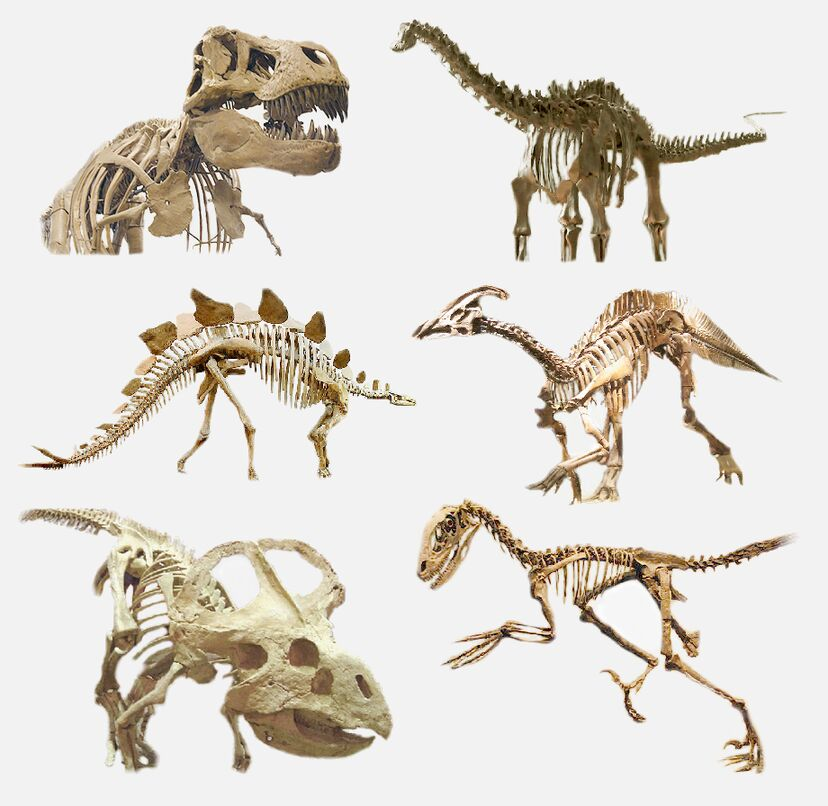
\includegraphics[max height=.45\textheight,
        max width=0.95\textwidth]{{Images/lizard}.jpg}
    \end{center}
    \end{column}
    \end{columns}
}
\end{frame}
\begin{frame}[t]{Round 2 --- Dinosaurs --- \mbox{Answer 2}}
\vspace{-0.5em}
\begin{block}{Question}
Which two people were the executive producers of the 1988 animated children's film about a group of dinosaurs, \emph{The Land Before Time}?
\end{block}

\visible<2->{
    \begin{columns}[T,totalwidth=\linewidth]
    \begin{column}{0.32\linewidth}
    \begin{block}{Answer}
    George Lucas and Steven Spielberg
    \end{block}
    \end{column}
    \begin{column}{0.65\linewidth}
    \begin{center}
    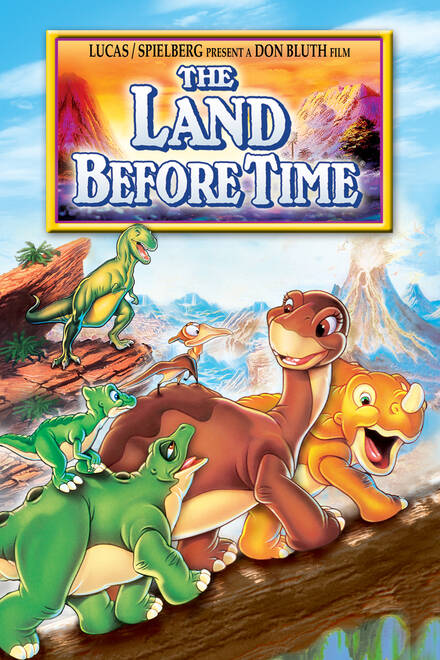
\includegraphics[max height=.45\textheight,
        max width=0.95\textwidth]{{Images/landbeforetime}.jpeg}
    \end{center}
    \end{column}
    \end{columns}
}
\end{frame}
\begin{frame}[t]{Round 2 --- Dinosaurs --- \mbox{Answer 3}}
\vspace{-0.5em}
\begin{block}{Question}
Which city does the NBA team The Raptors play in?
\end{block}

\visible<2->{
    \begin{columns}[T,totalwidth=\linewidth]
    \begin{column}{0.32\linewidth}
    \begin{block}{Answer}
    Toronto
    \end{block}
    \end{column}
    \begin{column}{0.65\linewidth}
    \begin{center}
    
\includegraphics[max height=.45\textheight,
        max width=0.95\textwidth]{{Images/raptors}.jpeg}
    \end{center}
    \end{column}
    \end{columns}
}
\end{frame}
\begin{frame}[t]{Round 2 --- Dinosaurs --- \mbox{Answer 4}}
\vspace{-0.5em}
\begin{block}{Question}
To within 5 million years, how many years ago were the (non-avian) dinosaurs wiped out by an asteroid?
\end{block}

\visible<2->{
    \begin{columns}[T,totalwidth=\linewidth]
    \begin{column}{0.32\linewidth}
    \begin{block}{Answer}
    65 million years ago (70--60 million years ago will be accepted)
    \end{block}
    \end{column}
    \begin{column}{0.65\linewidth}
    \begin{center}
    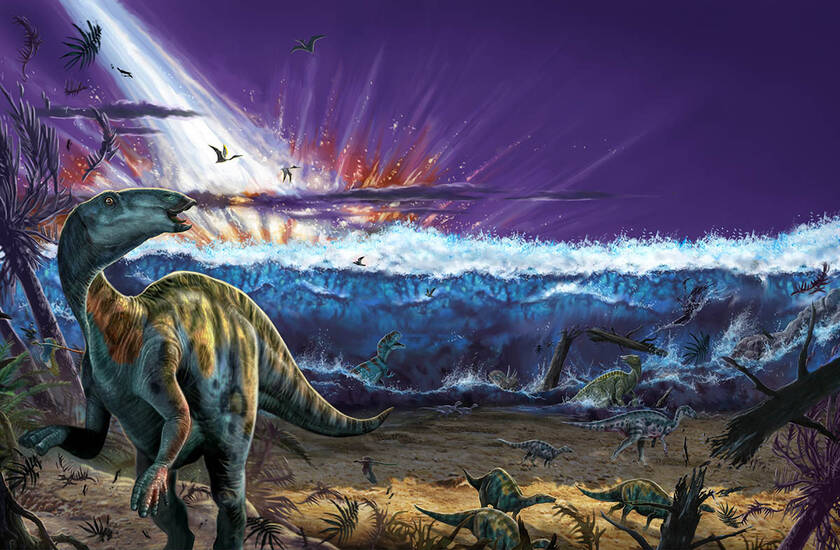
\includegraphics[max height=.45\textheight,
        max width=0.95\textwidth]{{Images/extinction}.jpeg}
    \end{center}
    \end{column}
    \end{columns}
}
\end{frame}
\begin{frame}[t]{Round 2 --- Dinosaurs --- \mbox{Answer 5}}
\vspace{-0.5em}
\begin{block}{Question}
Which large oil and gas company has a sauropod in its logo?
\end{block}

\visible<2->{
    \begin{columns}[T,totalwidth=\linewidth]
    \begin{column}{0.32\linewidth}
    \begin{block}{Answer}
    The Sinclair Oil Corporation / Sinclair
    \end{block}
    \end{column}
    \begin{column}{0.65\linewidth}
    \begin{center}
    
\includegraphics[max height=.45\textheight,
        max width=0.95\textwidth]{{Images/sinclair}.png}
    \end{center}
    \end{column}
    \end{columns}
}
\end{frame}
\begin{frame}[t]{Round 2 --- Dinosaurs --- \mbox{Answer 6}}
\vspace{-0.5em}
\begin{columns}[T,totalwidth=\linewidth]
\begin{column}{0.32\linewidth}
\begin{block}{Question}
Pictured here is an artist's rendition of which species of bird-like dinosaur that is generally believed to be the ancestor of all modern birds?
\end{block}
\visible<2->{
    \begin{block}{Answer}
    \emph{Archaeopteryx}
    \end{block}
}
\end{column}
\begin{column}{0.65\linewidth}
\begin{center}
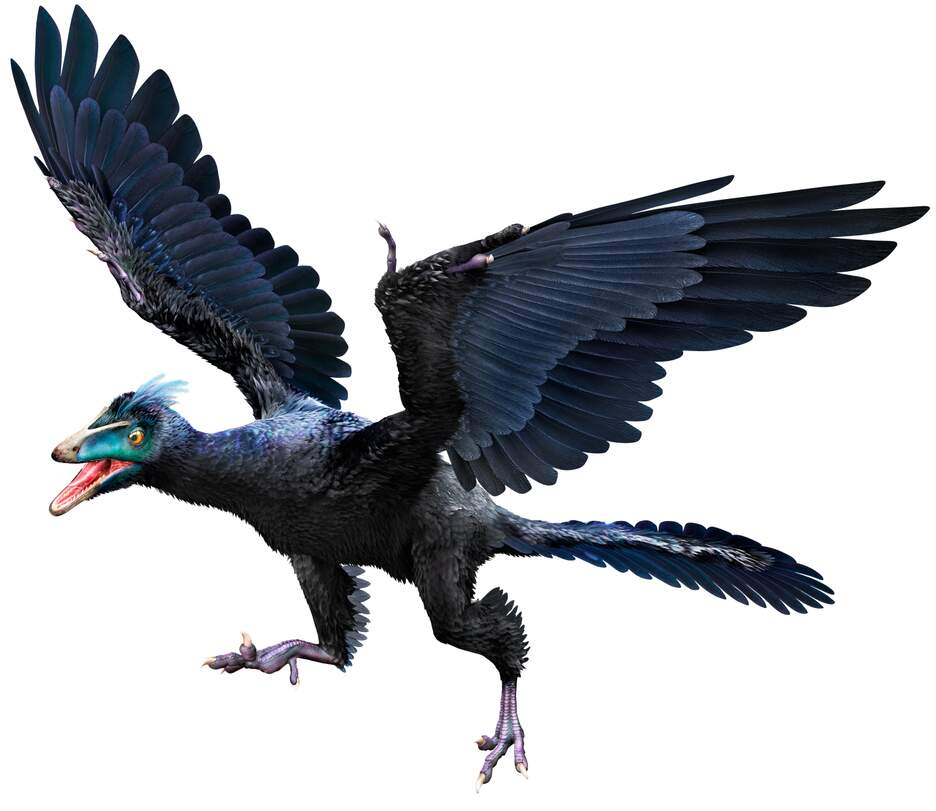
\includegraphics[max width=0.95\textwidth,max height=0.7\textheight]{{Images/archaeopteryx}.jpg}
\end{center}
\end{column}
\end{columns}
\end{frame}
\begin{frame}[t]{Round 2 --- Dinosaurs --- \mbox{Answer 7}}
\vspace{-0.5em}
\begin{block}{Question}
In what year was \emph{Jurassic Park} released?
\end{block}

\visible<2->{
    \begin{columns}[T,totalwidth=\linewidth]
    \begin{column}{0.32\linewidth}
    \begin{block}{Answer}
    1993
    \end{block}
    \end{column}
    \begin{column}{0.65\linewidth}
    \begin{center}
    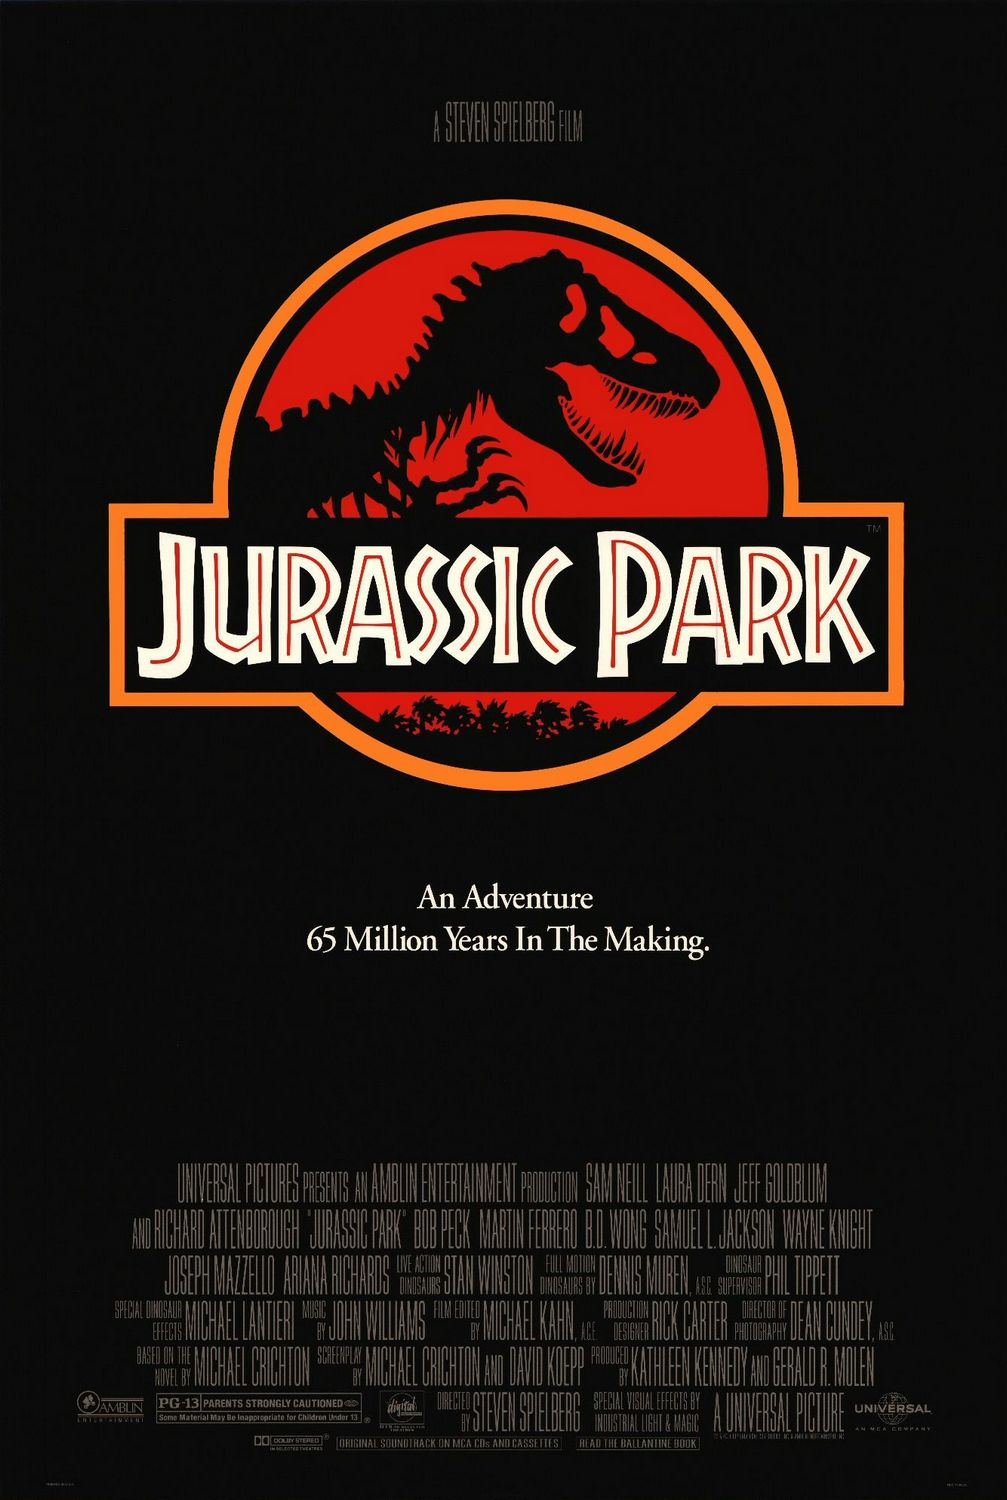
\includegraphics[max height=.45\textheight,
        max width=0.95\textwidth]{{Images/jurrassic}.jpeg}
    \end{center}
    \end{column}
    \end{columns}
}
\end{frame}
\begin{frame}[t]{Round 2 --- Dinosaurs --- \mbox{Answer 8}}
\vspace{-0.5em}
\begin{block}{Question}
On \emph{Pee-wee's Playhouse}, what was the name of Pee-wee Herman's dinosaur friend?
\end{block}

\visible<2->{
    \begin{columns}[T,totalwidth=\linewidth]
    \begin{column}{0.32\linewidth}
    \begin{block}{Answer}
    Pterri the Pterodactyl / Pterri (spelling doesn't count; anything pronounced ``Terry'' is fine, although the show does make clear that his name starts with a ``P'')
    \end{block}
    \end{column}
    \begin{column}{0.65\linewidth}
    \begin{center}
    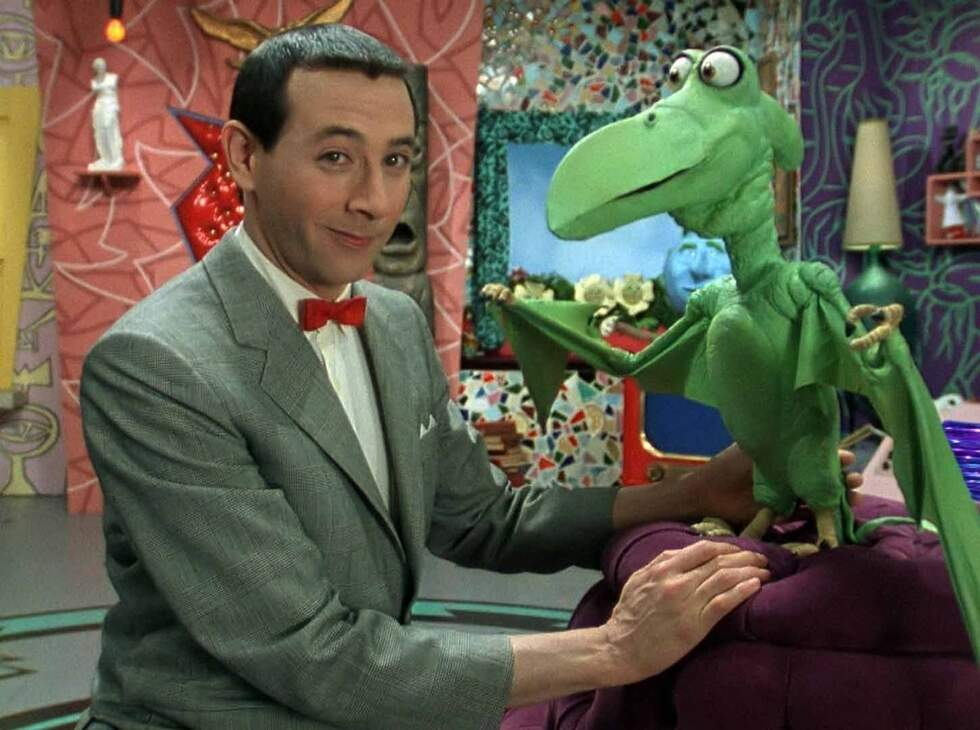
\includegraphics[max height=.45\textheight,
        max width=0.95\textwidth]{{Images/peewee}.jpg}
    \end{center}
    \end{column}
    \end{columns}
}
\end{frame}
\begin{frame}[t]{Round 2 --- Dinosaurs --- \mbox{Answer 9}}
\vspace{-0.5em}
\begin{columns}[T,totalwidth=\linewidth]
\begin{column}{0.32\linewidth}
\begin{block}{Question}
The skeleton of what kind of dinosaur is pictured here?
\end{block}
\visible<2->{
    \begin{block}{Answer}
    Stegosaurus
    \end{block}
}
\end{column}
\begin{column}{0.65\linewidth}
\begin{center}
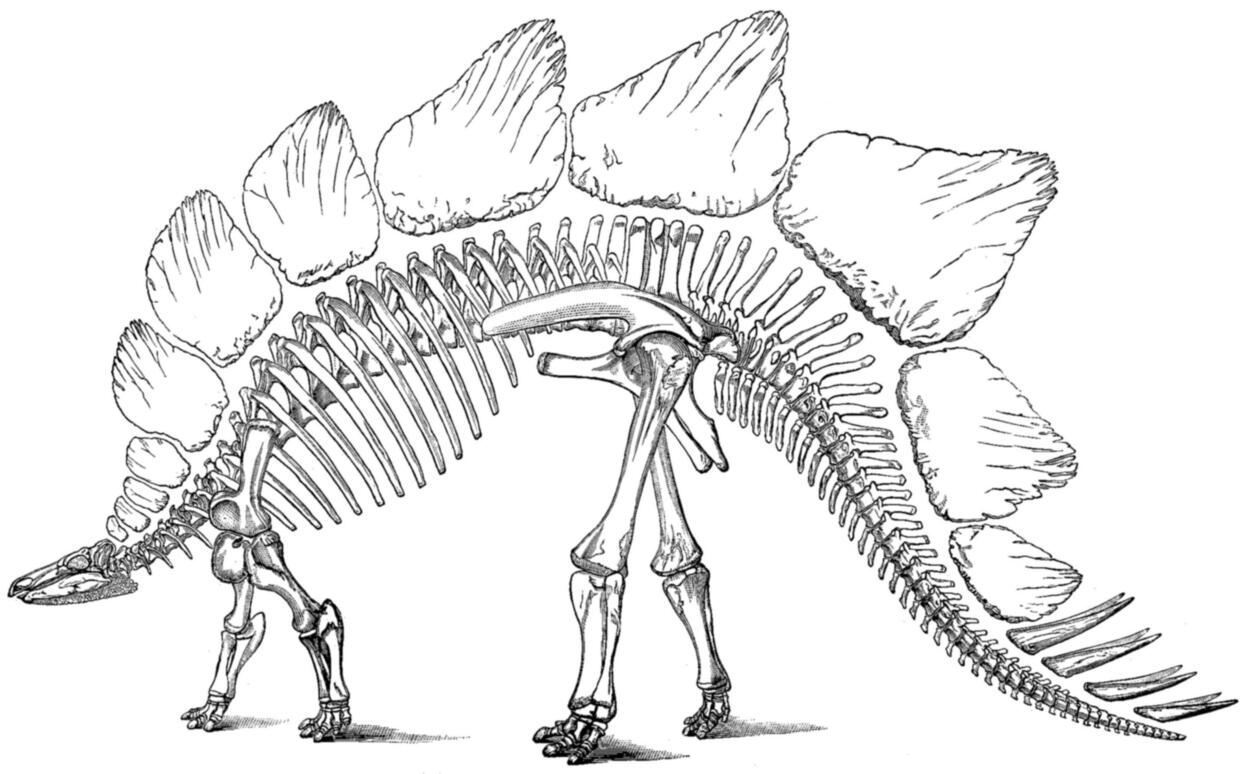
\includegraphics[max width=0.95\textwidth,max height=0.7\textheight]{{Images/stego}.jpg}
\end{center}
\end{column}
\end{columns}
\end{frame}
\begin{frame}[t]{Round 2 --- Dinosaurs --- \mbox{Answer 10}}
\vspace{-0.5em}
\begin{block}{Question}
What is the name of the period of intense, competitive hunting for dinosaur fossils that took place in the U.S. near the end of the 19\textsuperscript{th} Century?
\end{block}

\visible<2->{
    \begin{columns}[T,totalwidth=\linewidth]
    \begin{column}{0.54\linewidth}
    \begin{block}{Answer}
    The Bone Wars / The Great Dinosaur Rush (Edward Drinker Cope and Othniel Charles Marsh, pictured here, were the two biggest fossil hunters and were bitter rivals. They both went broke trying to outdo each other.)
    \end{block}
    \end{column}
    \begin{column}{0.42\linewidth}
    \begin{center}
    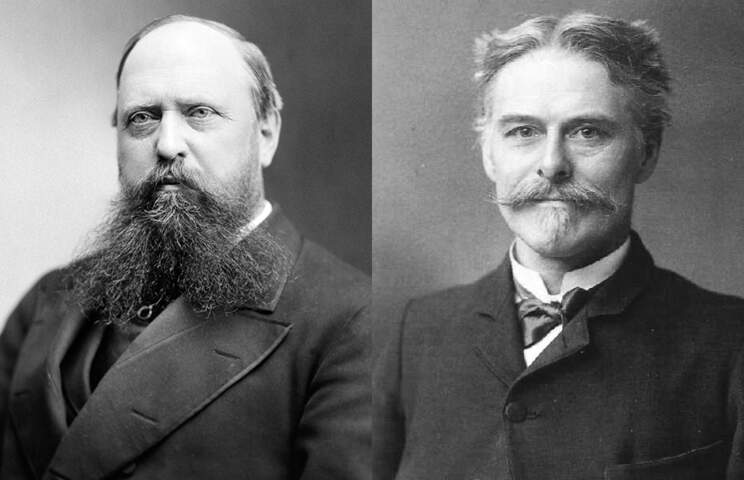
\includegraphics[max width=0.95\textwidth,
        max height=0.43000\textheight]{{Images/bonewars}.jpg}
    \end{center}
    \end{column}
    \end{columns}
}
\end{frame}
\def\thisSectionName{Political Slogans}
\section{Round 3}
\subsection*{Q1}
\begin{frame}[t]{Round 3 --- Political Slogans --- \mbox{Question 1}}
\vspace{-0.5em}
\begin{block}{Question}
In the slogan, ``Tippecanoe and Tyler too'', who was ``Tippecanoe''?
\end{block}
\end{frame}
\subsection*{Q2}
\begin{frame}[t]{Round 3 --- Political Slogans --- \mbox{Question 2}}
\vspace{-0.5em}
\begin{block}{Question}
``In your heart, you know he's right.''
\end{block}
\end{frame}
\subsection*{Q3}
\begin{frame}[t]{Round 3 --- Political Slogans --- \mbox{Question 3}}
\vspace{-0.5em}
\begin{block}{Question}
``A Time for Greatness''
\end{block}
\end{frame}
\subsection*{Q4}
\begin{frame}[t]{Round 3 --- Political Slogans --- \mbox{Question 4}}
\vspace{-0.5em}
\begin{block}{Question}
``This Time, Vote Like Your Whole World Depended on It''
\end{block}
\end{frame}
\subsection*{Q5}
\begin{frame}[t]{Round 3 --- Political Slogans --- \mbox{Question 5}}
\vspace{-0.5em}
\begin{block}{Question}
``A Leader, for a Change''
\end{block}
\end{frame}
\subsection*{Q6}
\begin{frame}[t]{Round 3 --- Political Slogans --- \mbox{Question 6}}
\vspace{-0.5em}
\begin{block}{Question}
``Change We Can Believe In''
\end{block}
\end{frame}
\subsection*{Q7}
\begin{frame}[t]{Round 3 --- Political Slogans --- \mbox{Question 7}}
\vspace{-0.5em}
\begin{block}{Question}
``A Chicken in Every Pot and a Car in Every Garage''
\end{block}
\end{frame}
\subsection*{Q8}
\begin{frame}[t]{Round 3 --- Political Slogans --- \mbox{Question 8}}
\vspace{-0.5em}
\begin{block}{Question}
``Don't Swap Horses in the Middle of the Stream''
\end{block}
\end{frame}
\subsection*{Q9}
\begin{frame}[t]{Round 3 --- Political Slogans --- \mbox{Question 9}}
\vspace{-0.5em}
\begin{block}{Question}
``Stronger Together''
\end{block}
\end{frame}
\subsection*{Q10}
\begin{frame}[t]{Round 3 --- Political Slogans --- \mbox{Question 10}}
\vspace{-0.5em}
\begin{block}{Question}
``I Like Ike'' 
\end{block}
\end{frame}
\subsection{Answers}
\begin{frame}[t]{Round 3 --- Political Slogans --- \mbox{Answer 1}}
\vspace{-0.5em}
\begin{block}{Question}
In the slogan, ``Tippecanoe and Tyler too'', who was ``Tippecanoe''?
\end{block}

\visible<2->{
    \begin{columns}[T,totalwidth=\linewidth]
    \begin{column}{0.32\linewidth}
    \begin{block}{Answer}
    William Henry Harrison
    \end{block}
    \end{column}
    \begin{column}{0.65\linewidth}
    \begin{center}
    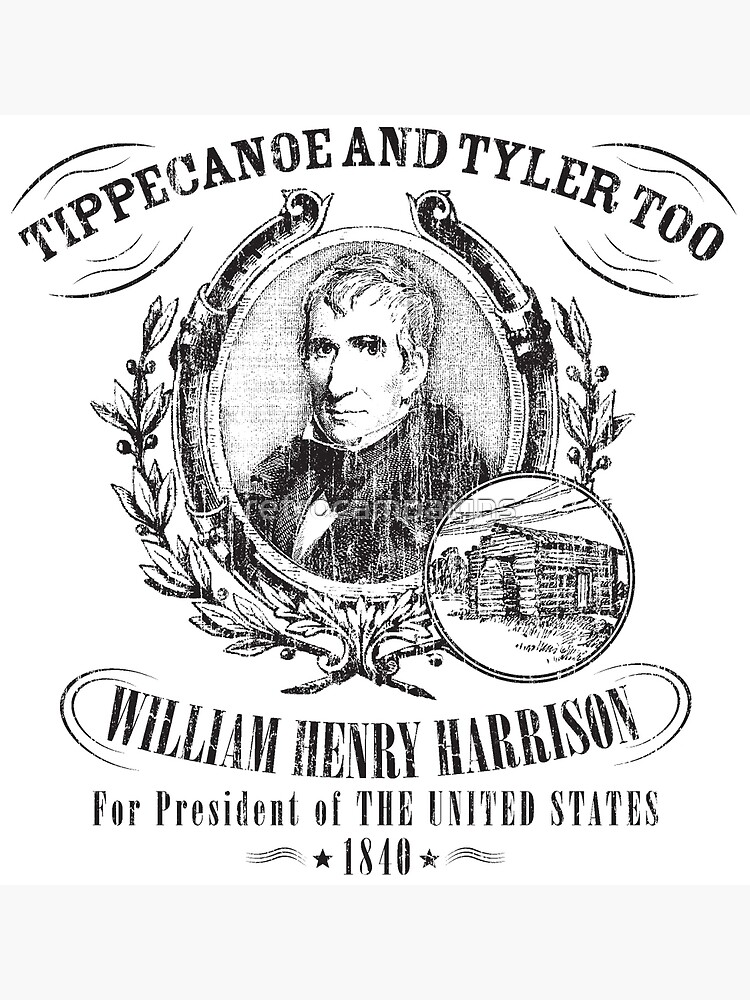
\includegraphics[max height=.45\textheight,
        max width=0.95\textwidth]{{Images/tippecanoe}.jpg}
    \end{center}
    \end{column}
    \end{columns}
}
\end{frame}
\begin{frame}[t]{Round 3 --- Political Slogans --- \mbox{Answer 2}}
\vspace{-0.5em}
\begin{block}{Question}
``In your heart, you know he's right.''
\end{block}

\visible<2->{
    \begin{columns}[T,totalwidth=\linewidth]
    \begin{column}{0.32\linewidth}
    \begin{block}{Answer}
    Barry Goldwater. (The slogan was parodied by the Democrats as ``In your guts, you know he's nuts.'')
    \end{block}
    \end{column}
    \begin{column}{0.65\linewidth}
    \begin{center}
    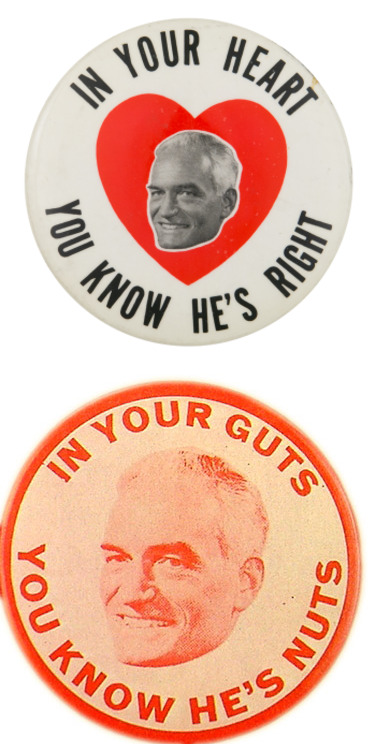
\includegraphics[max height=.45\textheight,
        max width=0.95\textwidth]{{Images/goldwater}.jpg}
    \end{center}
    \end{column}
    \end{columns}
}
\end{frame}
\begin{frame}[t]{Round 3 --- Political Slogans --- \mbox{Answer 3}}
\vspace{-0.5em}
\begin{block}{Question}
``A Time for Greatness''
\end{block}

\visible<2->{
    \begin{columns}[T,totalwidth=\linewidth]
    \begin{column}{0.32\linewidth}
    \begin{block}{Answer}
    John F. Kennedy
    \end{block}
    \end{column}
    \begin{column}{0.65\linewidth}
    \begin{center}
    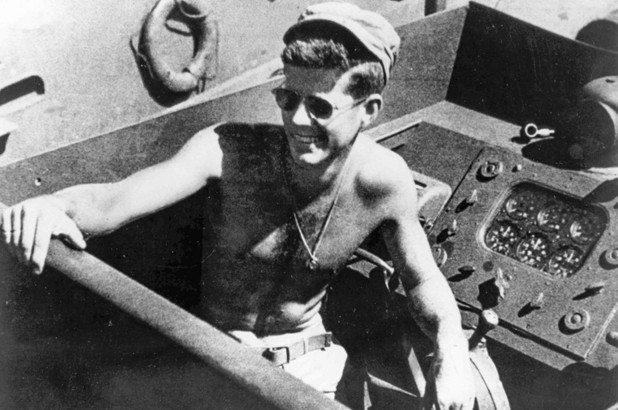
\includegraphics[max height=.45\textheight,
        max width=0.95\textwidth]{{Images/jfk}.jpg}
    \end{center}
    \end{column}
    \end{columns}
}
\end{frame}
\begin{frame}[t]{Round 3 --- Political Slogans --- \mbox{Answer 4}}
\vspace{-0.5em}
\begin{block}{Question}
``This Time, Vote Like Your Whole World Depended on It''
\end{block}

\visible<2->{
    \begin{columns}[T,totalwidth=\linewidth]
    \begin{column}{0.32\linewidth}
    \begin{block}{Answer}
    Richard M. Nixon
    \end{block}
    \end{column}
    \begin{column}{0.65\linewidth}
    \begin{center}
    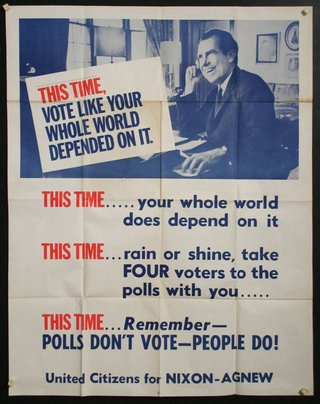
\includegraphics[max height=.45\textheight,
        max width=0.95\textwidth]{{Images/nixon}.jpg}
    \end{center}
    \end{column}
    \end{columns}
}
\end{frame}
\begin{frame}[t]{Round 3 --- Political Slogans --- \mbox{Answer 5}}
\vspace{-0.5em}
\begin{block}{Question}
``A Leader, for a Change''
\end{block}

\visible<2->{
    \begin{columns}[T,totalwidth=\linewidth]
    \begin{column}{0.32\linewidth}
    \begin{block}{Answer}
    Jimmy Carter
    \end{block}
    \end{column}
    \begin{column}{0.65\linewidth}
    \begin{center}
    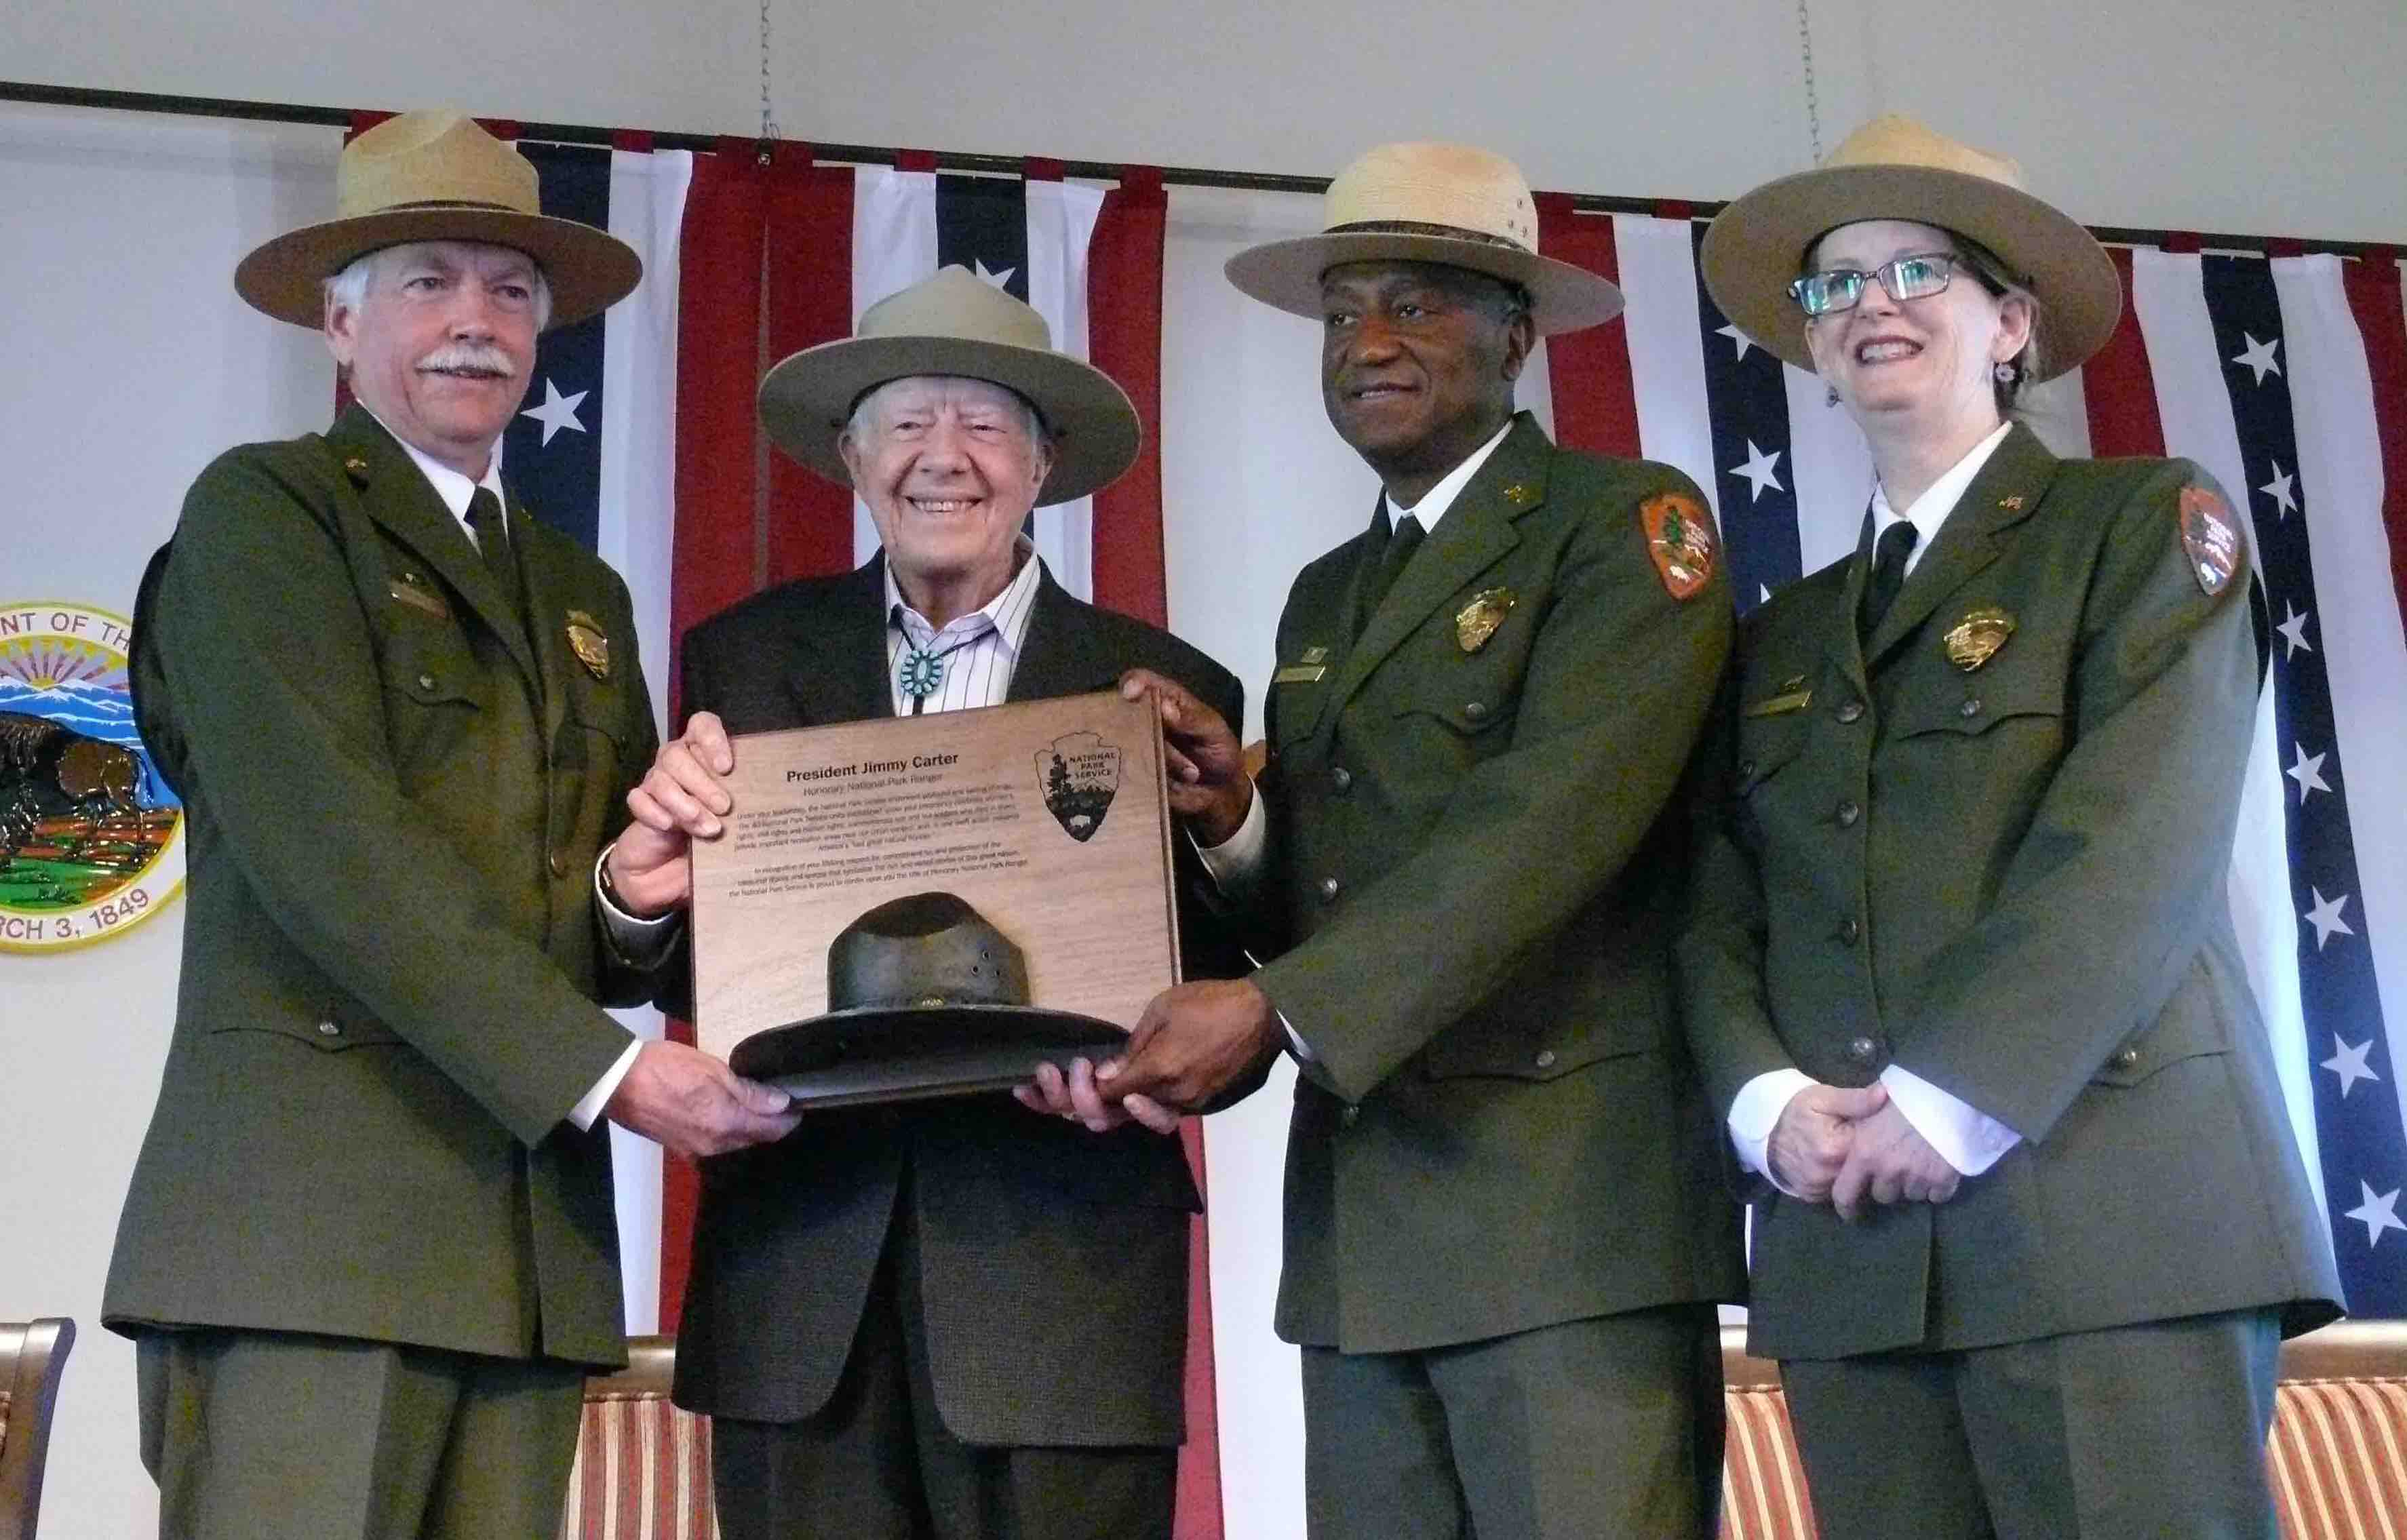
\includegraphics[max height=.45\textheight,
        max width=0.95\textwidth]{{Images/carter}.jpg}
    \end{center}
    \end{column}
    \end{columns}
}
\end{frame}
\begin{frame}[t]{Round 3 --- Political Slogans --- \mbox{Answer 6}}
\vspace{-0.5em}
\begin{block}{Question}
``Change We Can Believe In''
\end{block}

\visible<2->{
    \begin{columns}[T,totalwidth=\linewidth]
    \begin{column}{0.32\linewidth}
    \begin{block}{Answer}
    Barack Obama
    \end{block}
    \end{column}
    \begin{column}{0.65\linewidth}
    \begin{center}
    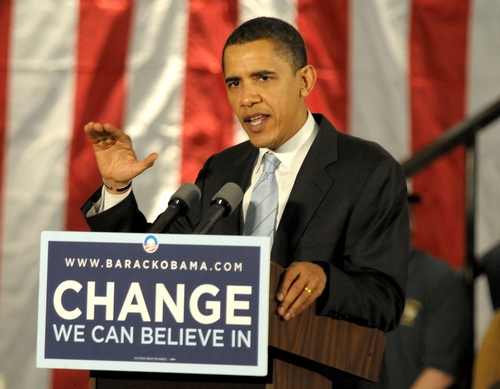
\includegraphics[max height=.45\textheight,
        max width=0.95\textwidth]{{Images/obama}.jpeg}
    \end{center}
    \end{column}
    \end{columns}
}
\end{frame}
\begin{frame}[t]{Round 3 --- Political Slogans --- \mbox{Answer 7}}
\vspace{-0.5em}
\begin{block}{Question}
``A Chicken in Every Pot and a Car in Every Garage''
\end{block}

\visible<2->{
    \begin{columns}[T,totalwidth=\linewidth]
    \begin{column}{0.32\linewidth}
    \begin{block}{Answer}
    Herbert Hoover
    \end{block}
    \end{column}
    \begin{column}{0.65\linewidth}
    \begin{center}
    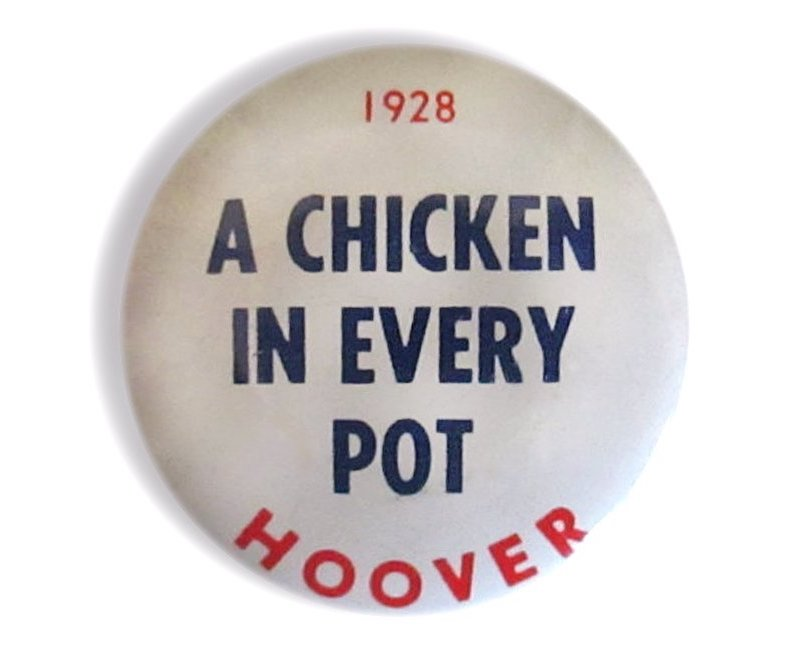
\includegraphics[max height=.45\textheight,
        max width=0.95\textwidth]{{Images/hoover}.jpg}
    \end{center}
    \end{column}
    \end{columns}
}
\end{frame}
\begin{frame}[t]{Round 3 --- Political Slogans --- \mbox{Answer 8}}
\vspace{-0.5em}
\begin{block}{Question}
``Don't Swap Horses in the Middle of the Stream''
\end{block}

\visible<2->{
    \begin{columns}[T,totalwidth=\linewidth]
    \begin{column}{0.32\linewidth}
    \begin{block}{Answer}
    Abraham Lincoln (1864 campaign)
    \end{block}
    \end{column}
    \begin{column}{0.65\linewidth}
    \begin{center}
    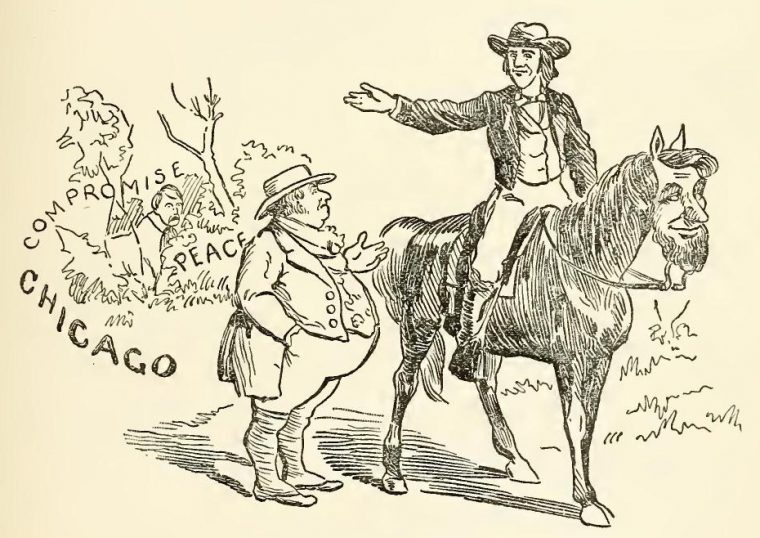
\includegraphics[max height=.45\textheight,
        max width=0.95\textwidth]{{Images/horse}.jpg}
    \end{center}
    \end{column}
    \end{columns}
}
\end{frame}
\begin{frame}[t]{Round 3 --- Political Slogans --- \mbox{Answer 9}}
\vspace{-0.5em}
\begin{block}{Question}
``Stronger Together''
\end{block}

\visible<2->{
    \begin{columns}[T,totalwidth=\linewidth]
    \begin{column}{0.32\linewidth}
    \begin{block}{Answer}
    Hillary Clinton
    \end{block}
    \end{column}
    \begin{column}{0.65\linewidth}
    \begin{center}
    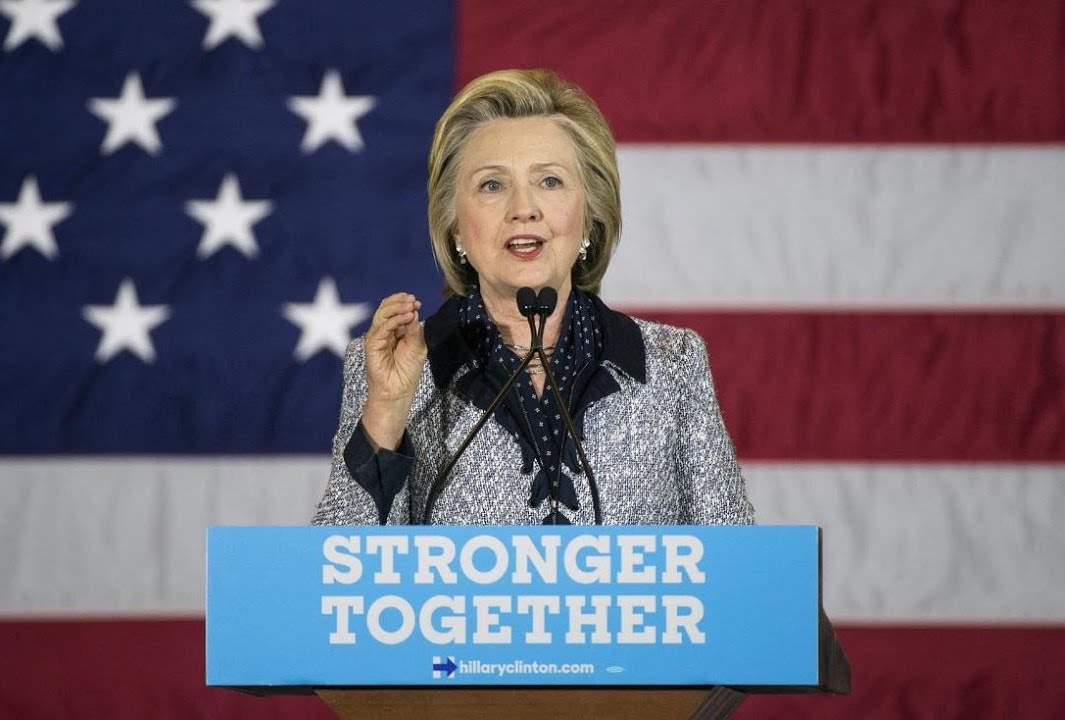
\includegraphics[max height=.45\textheight,
        max width=0.95\textwidth]{{Images/hillary}.jpeg}
    \end{center}
    \end{column}
    \end{columns}
}
\end{frame}
\begin{frame}[t]{Round 3 --- Political Slogans --- \mbox{Answer 10}}
\vspace{-0.5em}
\begin{block}{Question}
``I Like Ike'' 
\end{block}

\visible<2->{
    \begin{columns}[T,totalwidth=\linewidth]
    \begin{column}{0.32\linewidth}
    \begin{block}{Answer}
    Dwight D. Eisenhower
    \end{block}
    \end{column}
    \begin{column}{0.65\linewidth}
    \begin{center}
    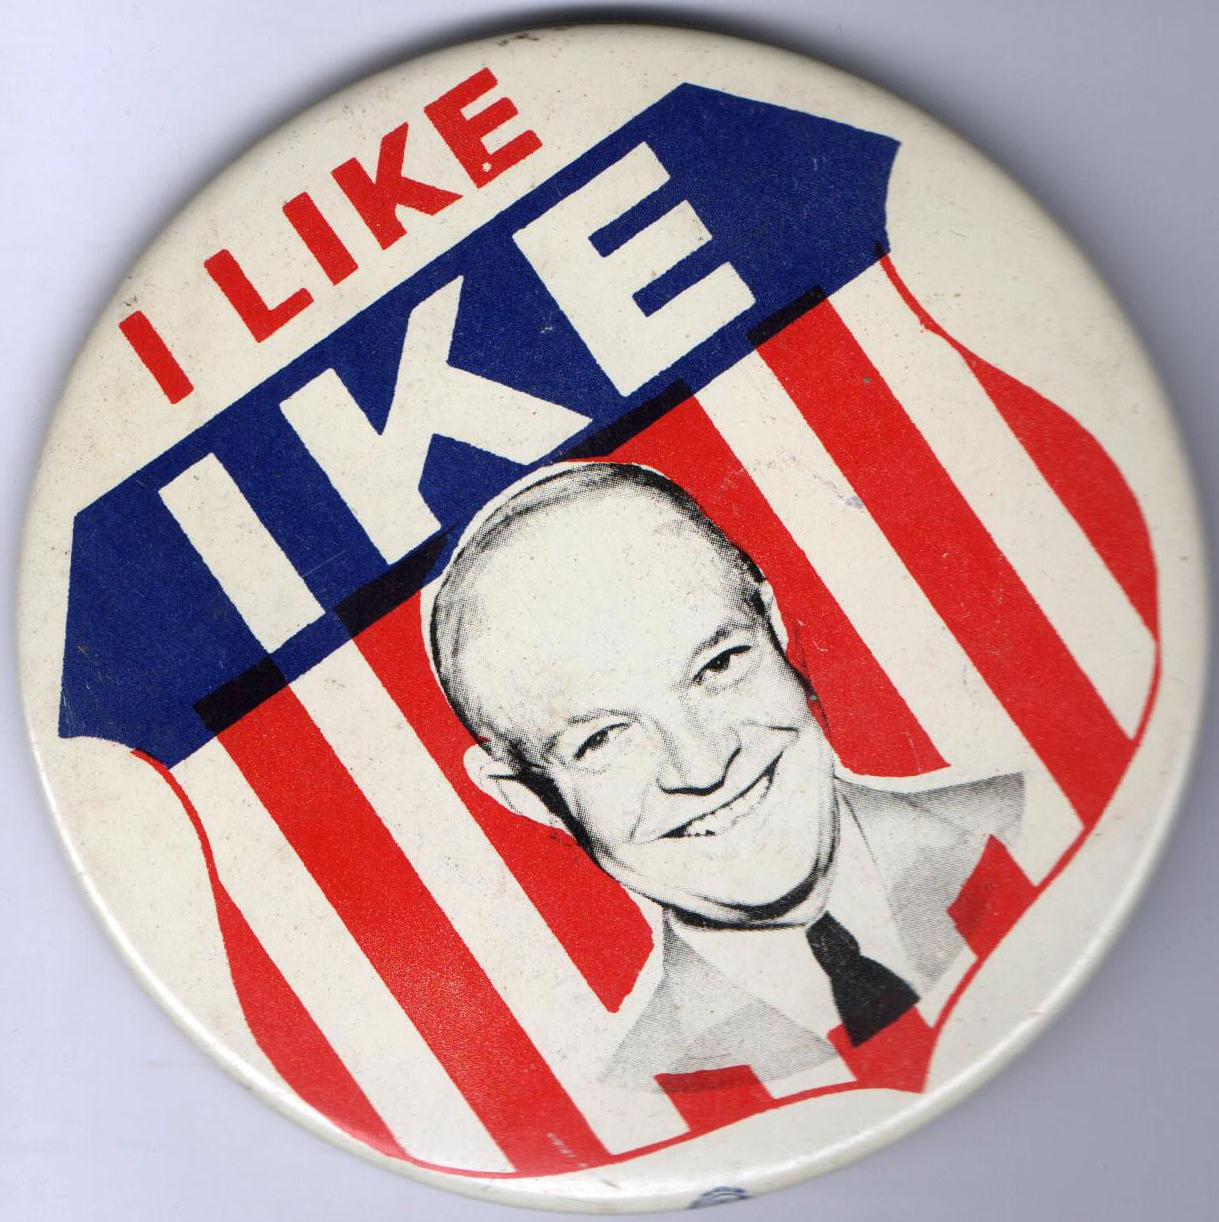
\includegraphics[max height=.45\textheight,
        max width=0.95\textwidth]{{Images/ike}.jpeg}
    \end{center}
    \end{column}
    \end{columns}
}
\end{frame}
\def\thisSectionName{I Love You, You're Perfect, Now be Past Perfect}
\section{Round 4}
\subsection*{Q1}
\begin{frame}[t]{Round 4 --- I Love You, You're Perfect, Now be Past Perfect --- \mbox{Question 1}}
\vspace{-0.5em}
\begin{block}{Question}
Name any three of the moods in the English language.
\end{block}
\end{frame}
\subsection*{Q2}
\begin{frame}[t]{Round 4 --- I Love You, You're Perfect, Now be Past Perfect --- \mbox{Question 2}}
\vspace{-0.5em}
\begin{block}{Question}
``To put up with'', ``to hand over'', and ``to back out of'' are examples of which kind of verbs? 
\end{block}
\end{frame}
\subsection*{Q3}
\begin{frame}[t]{Round 4 --- I Love You, You're Perfect, Now be Past Perfect --- \mbox{Question 3}}
\vspace{-0.5em}
\begin{block}{Question}
What have generations of English teachers admonished students not to dangle?
\end{block}
\end{frame}
\subsection*{Q4}
\begin{frame}[t]{Round 4 --- I Love You, You're Perfect, Now be Past Perfect --- \mbox{Question 4}}
\vspace{-0.5em}
\begin{block}{Question}
With almost 450 definitions, which English word has the most definitions in the \emph{Oxford English Dictionary}?
\end{block}
\end{frame}
\subsection*{Q5}
\begin{frame}[t]{Round 4 --- I Love You, You're Perfect, Now be Past Perfect --- \mbox{Question 5}}
\vspace{-0.5em}
\begin{block}{Question}
What is the word for a sentence that contains every letter of the alphabet, such as ``The quick brown fox jumps over the lazy dog''?
\end{block}
\end{frame}
\subsection*{Q6}
\begin{frame}[t]{Round 4 --- I Love You, You're Perfect, Now be Past Perfect --- \mbox{Question 6}}
\vspace{-0.5em}
\begin{block}{Question}
What is a ``contronym''?
\end{block}
\end{frame}
\subsection*{Q7}
\begin{frame}[t]{Round 4 --- I Love You, You're Perfect, Now be Past Perfect --- \mbox{Question 7}}
\vspace{-0.5em}
\begin{block}{Question}
Name five of the eight parts of speech in English.
\end{block}
\end{frame}
\subsection*{Q8}
\begin{frame}[t]{Round 4 --- I Love You, You're Perfect, Now be Past Perfect --- \mbox{Question 8}}
\vspace{-0.5em}
\begin{block}{Question}
What letter appears most frequently in English words?
\end{block}
\end{frame}
\subsection*{Q9}
\begin{frame}[t]{Round 4 --- I Love You, You're Perfect, Now be Past Perfect --- \mbox{Question 9}}
\vspace{-0.5em}
\begin{block}{Question}
What letter begins the most words in English?
\end{block}
\end{frame}
\subsection*{Q10}
\begin{frame}[t]{Round 4 --- I Love You, You're Perfect, Now be Past Perfect --- \mbox{Question 10}}
\vspace{-0.5em}
\begin{block}{Question}
What is the dot over the letter ``i'' called?
\end{block}
\end{frame}
\subsection{Answers}
\begin{frame}[t]{Round 4 --- I Love You, You're Perfect, Now be Past Perfect --- \mbox{Answer 1}}
\vspace{-0.5em}
\begin{block}{Question}
Name any three of the moods in the English language.
\end{block}
\visible<2->{
    \begin{block}{Answer}
    Indicative, imperative, conditional, interrogative, and subjunctive.  (We note that there is debate about whether or not the conditional and the interrogative are moods, but we will accept them. And we only needed three.)
    \end{block}
}
\end{frame}
\begin{frame}[t]{Round 4 --- I Love You, You're Perfect, Now be Past Perfect --- \mbox{Answer 2}}
\vspace{-0.5em}
\begin{block}{Question}
``To put up with'', ``to hand over'', and ``to back out of'' are examples of which kind of verbs? 
\end{block}
\visible<2->{
    \begin{block}{Answer}
    Phrasal verbs
    \end{block}
}
\end{frame}
\begin{frame}[t]{Round 4 --- I Love You, You're Perfect, Now be Past Perfect --- \mbox{Answer 3}}
\vspace{-0.5em}
\begin{block}{Question}
What have generations of English teachers admonished students not to dangle?
\end{block}
\visible<2->{
    \begin{block}{Answer}
    Participles / prepositions (we will accept either one)
    \end{block}
}
\end{frame}
\begin{frame}[t]{Round 4 --- I Love You, You're Perfect, Now be Past Perfect --- \mbox{Answer 4}}
\vspace{-0.5em}
\begin{block}{Question}
With almost 450 definitions, which English word has the most definitions in the \emph{Oxford English Dictionary}?
\end{block}
\visible<2->{
    \begin{block}{Answer}
    ``Set''
    \end{block}
}
\end{frame}
\begin{frame}[t]{Round 4 --- I Love You, You're Perfect, Now be Past Perfect --- \mbox{Answer 5}}
\vspace{-0.5em}
\begin{block}{Question}
What is the word for a sentence that contains every letter of the alphabet, such as ``The quick brown fox jumps over the lazy dog''?
\end{block}
\visible<2->{
    \begin{block}{Answer}
    Pangram
    \end{block}
}
\end{frame}
\begin{frame}[t]{Round 4 --- I Love You, You're Perfect, Now be Past Perfect --- \mbox{Answer 6}}
\vspace{-0.5em}
\begin{block}{Question}
What is a ``contronym''?
\end{block}
\visible<2->{
    \begin{block}{Answer}
    A verb that can have opposite meanings depending upon context. (For example, ``to dust'', ``to overlook'', and ``to sanction.'')
    \end{block}
}
\end{frame}
\begin{frame}[t]{Round 4 --- I Love You, You're Perfect, Now be Past Perfect --- \mbox{Answer 7}}
\vspace{-0.5em}
\begin{block}{Question}
Name five of the eight parts of speech in English.
\end{block}
\visible<2->{
    \begin{block}{Answer}
    Nouns, verbs, adjectives, adverbs, prepositions, conjunctions, articles and pronouns.
    \end{block}
}
\end{frame}
\begin{frame}[t]{Round 4 --- I Love You, You're Perfect, Now be Past Perfect --- \mbox{Answer 8}}
\vspace{-0.5em}
\begin{block}{Question}
What letter appears most frequently in English words?
\end{block}
\visible<2->{
    \begin{block}{Answer}
    ``E''
    \end{block}
}
\end{frame}
\begin{frame}[t]{Round 4 --- I Love You, You're Perfect, Now be Past Perfect --- \mbox{Answer 9}}
\vspace{-0.5em}
\begin{block}{Question}
What letter begins the most words in English?
\end{block}
\visible<2->{
    \begin{block}{Answer}
    ``S''
    \end{block}
}
\end{frame}
\begin{frame}[t]{Round 4 --- I Love You, You're Perfect, Now be Past Perfect --- \mbox{Answer 10}}
\vspace{-0.5em}
\begin{block}{Question}
What is the dot over the letter ``i'' called?
\end{block}
\visible<2->{
    \begin{block}{Answer}
    A tittle
    \end{block}
}
\end{frame}
\def\thisSectionName{Number One Songs}
\section{Round 5}
\subsection*{Q1}
\begin{frame}[t]{Round 5 --- Number One Songs --- \mbox{Question 1}}
\vspace{-0.5em}
\begin{block}{Question}
What 1977 song was the first song to stay \#1 on the Billboard Hot 100 for 10 weeks?
\end{block}
\end{frame}
\subsection*{Q2}
\begin{frame}[t]{Round 5 --- Number One Songs --- \mbox{Question 2}}
\vspace{-0.5em}
\begin{block}{Question}
To within two, how many Rolling Stones songs hit \#1?
\end{block}
\end{frame}
\subsection*{Q3}
\begin{frame}[t]{Round 5 --- Number One Songs --- \mbox{Question 3}}
\vspace{-0.5em}
\begin{block}{Question}
Which musician --- with a total of 10 \#1 hits on the Billboard Hot 100 --- had his first \#1 hit when he was just 13?
\end{block}
\end{frame}
\subsection*{Q4}
\begin{frame}[t]{Round 5 --- Number One Songs --- \mbox{Question 4}}
\vspace{-0.5em}
\begin{block}{Question}
Which song about martial arts reached the \#1 spot in 1974?
\end{block}
\end{frame}
\subsection*{Q5}
\begin{frame}[t]{Round 5 --- Number One Songs --- \mbox{Question 5}}
\vspace{-0.5em}
\begin{block}{Question}
The band Los Del Rio is best known for which 1996 \#1 song that kicked off a dance craze?
\end{block}
\end{frame}
\subsection*{Q6}
\begin{frame}[t]{Round 5 --- Number One Songs --- \mbox{Question 6}}
\vspace{-0.5em}
\begin{block}{Question}
Which Italian-language song hit the \#1 spot in 1958?
\end{block}
\end{frame}
\subsection*{Q7}
\begin{frame}[t]{Round 5 --- Number One Songs --- \mbox{Question 7}}
\vspace{-0.5em}
\begin{block}{Question}
Only one Aerosmith song reached \#1 on the Billboard Hot 100.  Which song was it?
\end{block}
\end{frame}
\subsection*{Q8}
\begin{frame}[t]{Round 5 --- Number One Songs --- \mbox{Question 8}}
\vspace{-0.5em}
\begin{block}{Question}
Name the two Adele songs that hit \#1 in 2011.
\end{block}
\end{frame}
\subsection*{Q9}
\begin{frame}[t]{Round 5 --- Number One Songs --- \mbox{Question 9}}
\vspace{-0.5em}
\begin{block}{Question}
Name three of the five singers/groups with the most \#1 hits of all time.
\end{block}
\end{frame}
\subsection*{Q10}
\begin{frame}[t]{Round 5 --- Number One Songs --- \mbox{Question 10}}
\vspace{-0.5em}
\begin{block}{Question}
Which Ricky Nelson song from 1958 --- the year that the Billboard Hot 100 was introduced --- was the very first Billboard Hot 100 \#1 song?
\end{block}
\end{frame}
\subsection{Answers}
\begin{frame}[t]{Round 5 --- Number One Songs --- \mbox{Answer 1}}
\vspace{-0.5em}
\begin{block}{Question}
What 1977 song was the first song to stay \#1 on the Billboard Hot 100 for 10 weeks?
\end{block}

\visible<2->{
    \begin{columns}[T,totalwidth=\linewidth]
    \begin{column}{0.32\linewidth}
    \begin{block}{Answer}
    You Light Up My Life (Debbie Boone)
    \end{block}
    \end{column}
    \begin{column}{0.65\linewidth}
    \begin{center}
    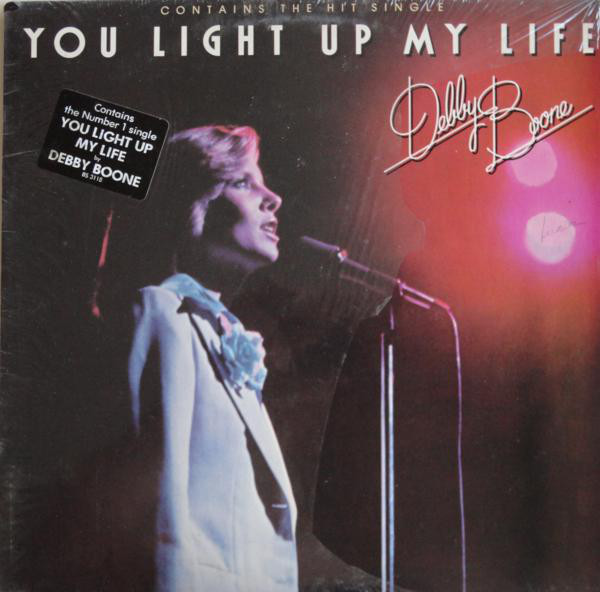
\includegraphics[max height=.45\textheight,
        max width=0.95\textwidth]{{Images/debbieboone}.jpg}
    \end{center}
    \end{column}
    \end{columns}
}
\end{frame}
\begin{frame}[t]{Round 5 --- Number One Songs --- \mbox{Answer 2}}
\vspace{-0.5em}
\begin{block}{Question}
To within two, how many Rolling Stones songs hit \#1?
\end{block}

\visible<2->{
    \begin{columns}[T,totalwidth=\linewidth]
    \begin{column}{0.32\linewidth}
    \begin{block}{Answer}
    8 (6 to 10 will be accepted)
    \end{block}
    \end{column}
    \begin{column}{0.65\linewidth}
    \begin{center}
    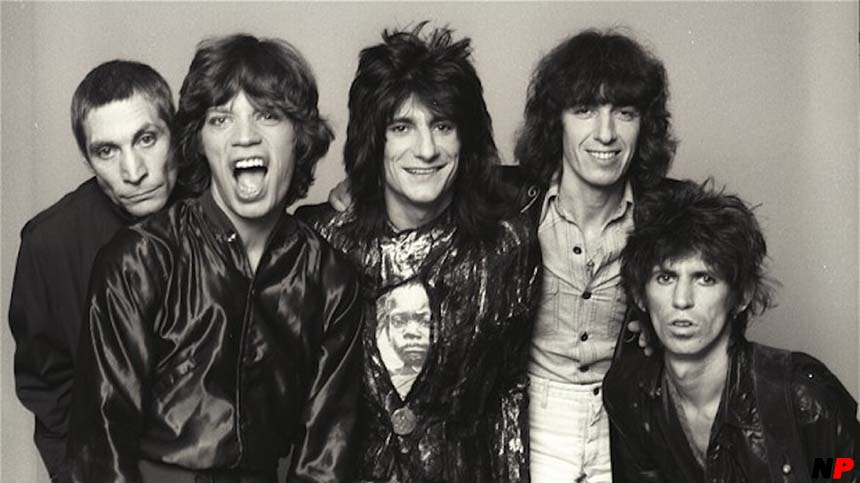
\includegraphics[max height=.45\textheight,
        max width=0.95\textwidth]{{Images/stones}.jpg}
    \end{center}
    \end{column}
    \end{columns}
}
\end{frame}
\begin{frame}[t]{Round 5 --- Number One Songs --- \mbox{Answer 3}}
\vspace{-0.5em}
\begin{block}{Question}
Which musician --- with a total of 10 \#1 hits on the Billboard Hot 100 --- had his first \#1 hit when he was just 13?
\end{block}

\visible<2->{
    \begin{columns}[T,totalwidth=\linewidth]
    \begin{column}{0.32\linewidth}
    \begin{block}{Answer}
    Stevie Wonder (``Fingertips'')
    \end{block}
    \end{column}
    \begin{column}{0.65\linewidth}
    \begin{center}
    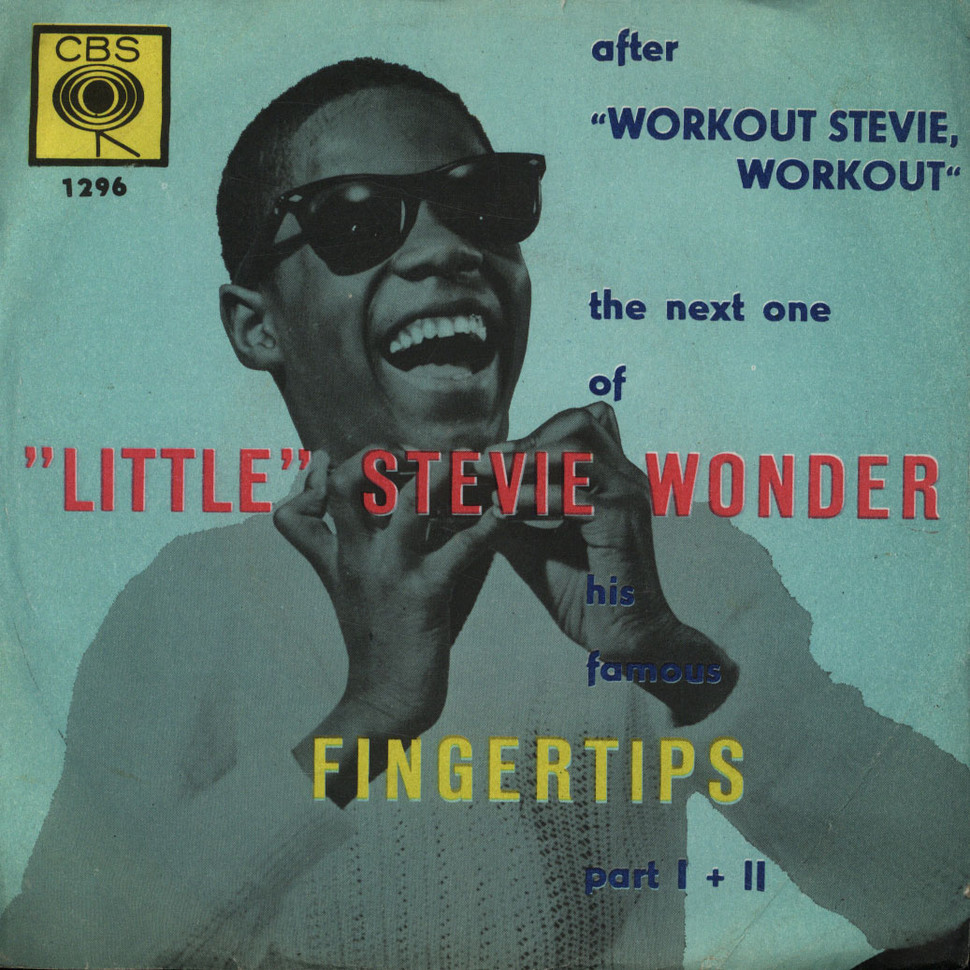
\includegraphics[max height=.45\textheight,
        max width=0.95\textwidth]{{Images/wonder}.jpeg}
    \end{center}
    \end{column}
    \end{columns}
}
\end{frame}
\begin{frame}[t]{Round 5 --- Number One Songs --- \mbox{Answer 4}}
\vspace{-0.5em}
\begin{block}{Question}
Which song about martial arts reached the \#1 spot in 1974?
\end{block}

\visible<2->{
    \begin{columns}[T,totalwidth=\linewidth]
    \begin{column}{0.32\linewidth}
    \begin{block}{Answer}
    ``(Everybody Was) Kung Fu Fighting''
    \end{block}
    \end{column}
    \begin{column}{0.65\linewidth}
    \begin{center}
    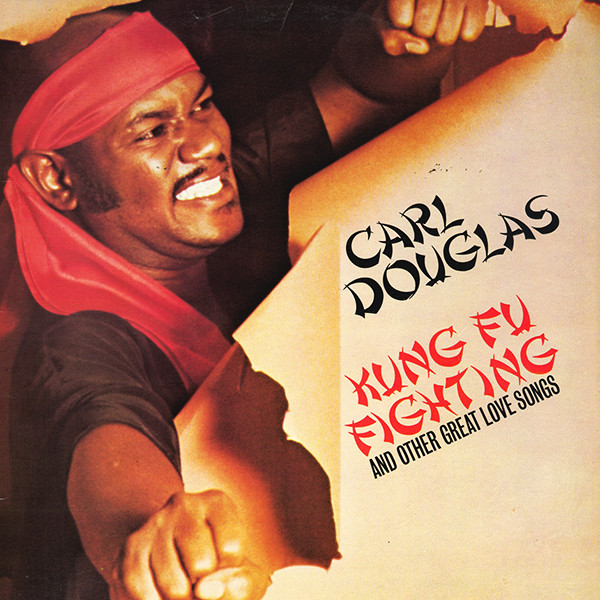
\includegraphics[max height=.45\textheight,
        max width=0.95\textwidth]{{Images/kungfu}.jpg}
    \end{center}
    \end{column}
    \end{columns}
}
\end{frame}
\begin{frame}[t]{Round 5 --- Number One Songs --- \mbox{Answer 5}}
\vspace{-0.5em}
\begin{block}{Question}
The band Los Del Rio is best known for which 1996 \#1 song that kicked off a dance craze?
\end{block}

\visible<2->{
    \begin{columns}[T,totalwidth=\linewidth]
    \begin{column}{0.32\linewidth}
    \begin{block}{Answer}
    The Macarena / ``Macarena (Bayside Boys Mix)''
    \end{block}
    \end{column}
    \begin{column}{0.65\linewidth}
    \begin{center}
    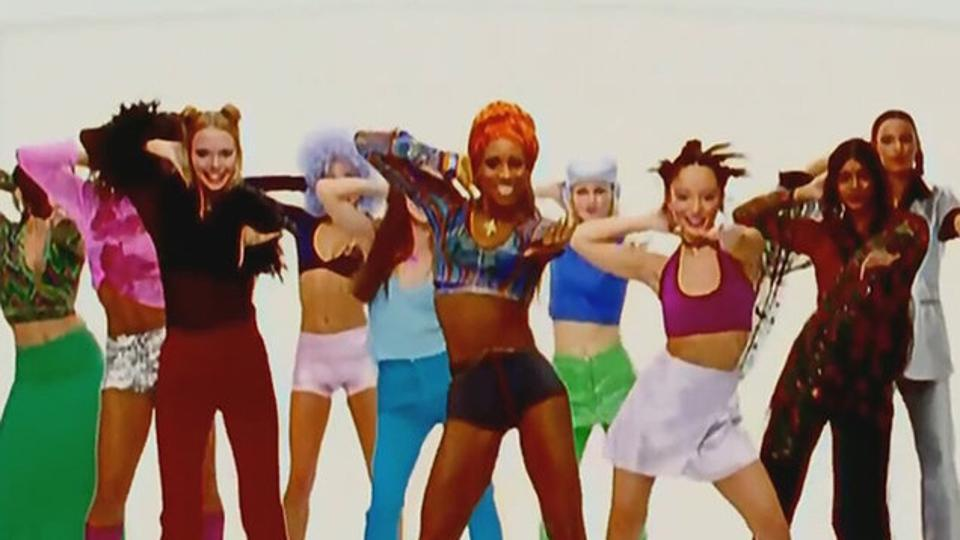
\includegraphics[max height=.45\textheight,
        max width=0.95\textwidth]{{Images/macarena}.jpg}
    \end{center}
    \end{column}
    \end{columns}
}
\end{frame}
\begin{frame}[t]{Round 5 --- Number One Songs --- \mbox{Answer 6}}
\vspace{-0.5em}
\begin{block}{Question}
Which Italian-language song hit the \#1 spot in 1958?
\end{block}

\visible<2->{
    \begin{columns}[T,totalwidth=\linewidth]
    \begin{column}{0.32\linewidth}
    \begin{block}{Answer}
    ``Volare'' / ``Nel blu, dipinto di blu'' (by Domenico Modugno)
    \end{block}
    \end{column}
    \begin{column}{0.65\linewidth}
    \begin{center}
    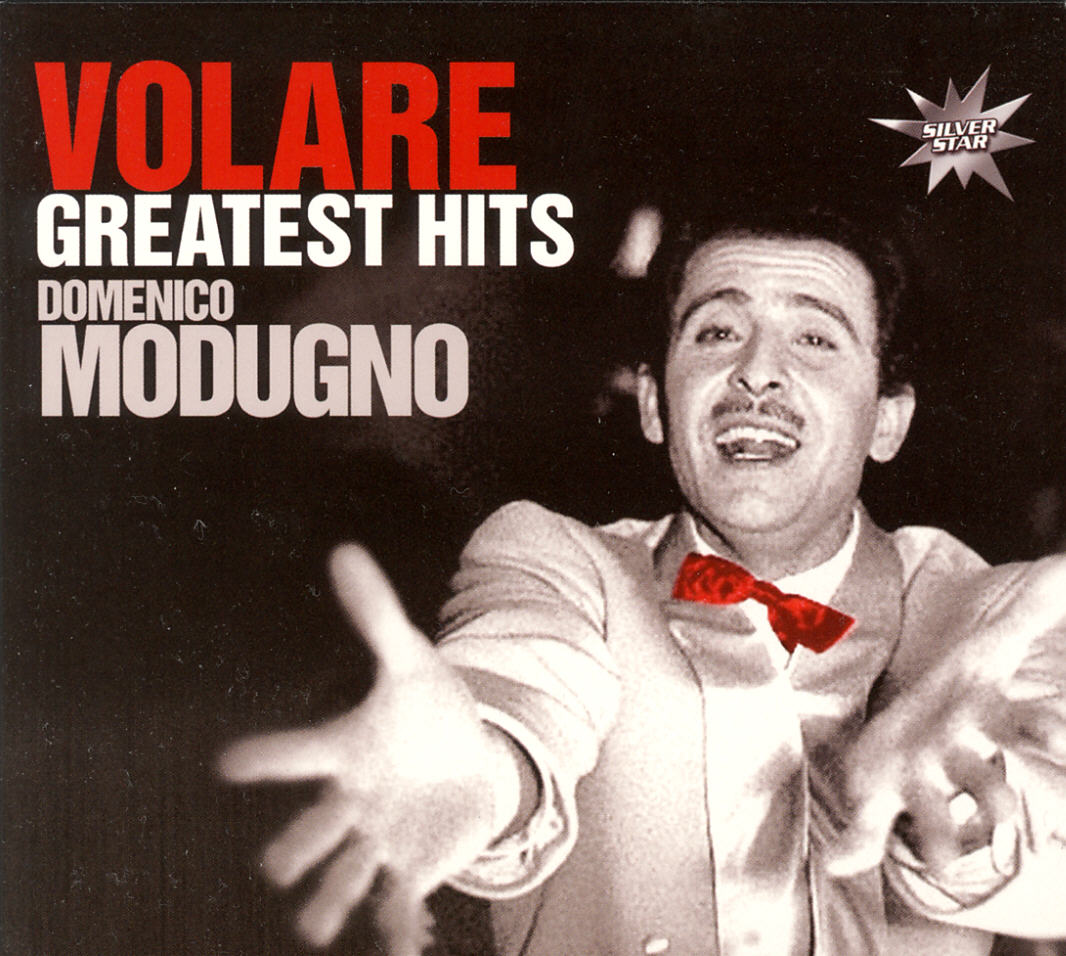
\includegraphics[max height=.45\textheight,
        max width=0.95\textwidth]{{Images/volare}.jpeg}
    \end{center}
    \end{column}
    \end{columns}
}
\end{frame}
\begin{frame}[t]{Round 5 --- Number One Songs --- \mbox{Answer 7}}
\vspace{-0.5em}
\begin{block}{Question}
Only one Aerosmith song reached \#1 on the Billboard Hot 100.  Which song was it?
\end{block}

\visible<2->{
    \begin{columns}[T,totalwidth=\linewidth]
    \begin{column}{0.32\linewidth}
    \begin{block}{Answer}
    ``I Don't Want to Miss a Thing''
    \end{block}
    \end{column}
    \begin{column}{0.65\linewidth}
    \begin{center}
    \includegraphics[max height=.45\textheight,
        max width=0.95\textwidth]{{Images/aero}.jpg}
    \end{center}
    \end{column}
    \end{columns}
}
\end{frame}
\begin{frame}[t]{Round 5 --- Number One Songs --- \mbox{Answer 8}}
\vspace{-0.5em}
\begin{block}{Question}
Name the two Adele songs that hit \#1 in 2011.
\end{block}

\visible<2->{
    \begin{columns}[T,totalwidth=\linewidth]
    \begin{column}{0.32\linewidth}
    \begin{block}{Answer}
    ``Rolling in the Deep'' and ``Someone Like You''
    \end{block}
    \end{column}
    \begin{column}{0.65\linewidth}
    \begin{center}
    \includegraphics[max height=.45\textheight,
        max width=0.95\textwidth]{{Images/adele}.jpeg}
    \end{center}
    \end{column}
    \end{columns}
}
\end{frame}
\begin{frame}[t]{Round 5 --- Number One Songs --- \mbox{Answer 9}}
\vspace{-0.5em}
\begin{block}{Question}
Name three of the five singers/groups with the most \#1 hits of all time.
\end{block}
\visible<2->{
    \begin{block}{Answer}
    No.\ 5, Michael Jackson; No.\ 4, Rihanna; No.\ 3, Elvis; No.\ 2, Mariah Carey; No.\ 1, The Beatles
    \end{block}
}
\end{frame}
\begin{frame}[t]{Round 5 --- Number One Songs --- \mbox{Answer 10}}
\vspace{-0.5em}
\begin{block}{Question}
Which Ricky Nelson song from 1958 --- the year that the Billboard Hot 100 was introduced --- was the very first Billboard Hot 100 \#1 song?
\end{block}

\visible<2->{
    \begin{columns}[T,totalwidth=\linewidth]
    \begin{column}{0.32\linewidth}
    \begin{block}{Answer}
    ``Poor Little Fool''
    \end{block}
    \end{column}
    \begin{column}{0.65\linewidth}
    \begin{center}
    \includegraphics[max height=.45\textheight,
        max width=0.95\textwidth]{{Images/nelson}.jpg}
    \end{center}
    \end{column}
    \end{columns}
}
\end{frame}
\def\thisSectionName{Things Dean Martin Never Said}
\section{Round 6}
\subsection*{Q1}
\begin{frame}[t]{Round 6 --- Things Dean Martin Never Said --- \mbox{Question 1}}
\vspace{-0.5em}
\begin{block}{Question}
Dean Martin might have been clever, but he wasn't clever enough to have said ``I am so clever that sometimes I don't understand a single word of what I am saying.'' Who did say it?
\end{block}
\end{frame}
\subsection*{Q2}
\begin{frame}[t]{Round 6 --- Things Dean Martin Never Said --- \mbox{Question 2}}
\vspace{-0.5em}
\begin{block}{Question}
Dean Martin wasn't a social change leader, so he never said ``The future belongs to those who prepare for it today.'' Who did?
\end{block}
\end{frame}
\subsection*{Q3}
\begin{frame}[t]{Round 6 --- Things Dean Martin Never Said --- \mbox{Question 3}}
\vspace{-0.5em}
\begin{block}{Question}
Dean Martin was too fashionable a dresser to say ``Once you can accept the universe as matter expanding into nothing that is something, wearing stripes with plaid comes easy.'' Who did say it?
\end{block}
\end{frame}
\subsection*{Q4}
\begin{frame}[t]{Round 6 --- Things Dean Martin Never Said --- \mbox{Question 4}}
\vspace{-0.5em}
\begin{block}{Question}
Dean Martin summed up life by saying ``When the moon hits your eye like a big pizza pie, that's amore'', so he didn't need to say, ``I wished to live deliberately, to front only the essential facts of life, and see if I could not learn what it had to teach, and not, when I came to die, discover that I had not lived.'' Who did say it?
\end{block}
\end{frame}
\subsection*{Q5}
\begin{frame}[t]{Round 6 --- Things Dean Martin Never Said --- \mbox{Question 5}}
\vspace{-0.5em}
\begin{block}{Question}
Dean Martin wasn't a dogged inventor, so he never said ``Many of life's failures are people who did not realize how close they were to success when they gave up.'' Who did?
\end{block}
\end{frame}
\subsection*{Q6}
\begin{frame}[t]{Round 6 --- Things Dean Martin Never Said --- \mbox{Question 6}}
\vspace{-0.5em}
\begin{block}{Question}
Dean Martin wasn't much of a philosopher, so he never said ``I think, therefore I am.'' Who did?
\end{block}
\end{frame}
\subsection*{Q7}
\begin{frame}[t]{Round 6 --- Things Dean Martin Never Said --- \mbox{Question 7}}
\vspace{-0.5em}
\begin{block}{Question}
Dean Martin was a man of scruples, so he never said, ``Those are my principles, and if you don't like them\ldots{} well, I have others.'' Who did?
\end{block}
\end{frame}
\subsection*{Q8}
\begin{frame}[t]{Round 6 --- Things Dean Martin Never Said --- \mbox{Question 8}}
\vspace{-0.5em}
\begin{block}{Question}
Dean Martin spoke Italian and English but not Greek, so he could have coined the phrase ``It was Greek to me'', but someone else did. Who?
\end{block}
\end{frame}
\subsection*{Q9}
\begin{frame}[t]{Round 6 --- Things Dean Martin Never Said --- \mbox{Question 9}}
\vspace{-0.5em}
\begin{block}{Question}
Dean Martin wasn't an author of fantasy literature, so he never wrote the line ``Not all those who wander are lost''. Who did?
\end{block}
\end{frame}
\subsection*{Q10}
\begin{frame}[t]{Round 6 --- Things Dean Martin Never Said --- \mbox{Question 10}}
\vspace{-0.5em}
\begin{block}{Question}
Dean Martin was handsome, so he never responded to being called ``two-faced'' by saying, ``If I were two-faced, would I be wearing this one?'' Who did?
\end{block}
\end{frame}
\subsection{Answers}
\begin{frame}[t]{Round 6 --- Things Dean Martin Never Said --- \mbox{Answer 1}}
\vspace{-0.5em}
\begin{block}{Question}
Dean Martin might have been clever, but he wasn't clever enough to have said ``I am so clever that sometimes I don't understand a single word of what I am saying.'' Who did say it?
\end{block}

\visible<2->{
    \begin{columns}[T,totalwidth=\linewidth]
    \begin{column}{0.32\linewidth}
    \begin{block}{Answer}
    Oscar Wilde
    \end{block}
    \end{column}
    \begin{column}{0.65\linewidth}
    \begin{center}
    \includegraphics[max height=.45\textheight,
        max width=0.95\textwidth]{{Images/wilde}.jpg}
    \end{center}
    \end{column}
    \end{columns}
}
\end{frame}
\begin{frame}[t]{Round 6 --- Things Dean Martin Never Said --- \mbox{Answer 2}}
\vspace{-0.5em}
\begin{block}{Question}
Dean Martin wasn't a social change leader, so he never said ``The future belongs to those who prepare for it today.'' Who did?
\end{block}

\visible<2->{
    \begin{columns}[T,totalwidth=\linewidth]
    \begin{column}{0.32\linewidth}
    \begin{block}{Answer}
    Malcom X
    \end{block}
    \end{column}
    \begin{column}{0.65\linewidth}
    \begin{center}
    \includegraphics[max height=.45\textheight,
        max width=0.95\textwidth]{{Images/malcomx}.jpg}
    \end{center}
    \end{column}
    \end{columns}
}
\end{frame}
\begin{frame}[t]{Round 6 --- Things Dean Martin Never Said --- \mbox{Answer 3}}
\vspace{-0.5em}
\begin{block}{Question}
Dean Martin was too fashionable a dresser to say ``Once you can accept the universe as matter expanding into nothing that is something, wearing stripes with plaid comes easy.'' Who did say it?
\end{block}

\visible<2->{
    \begin{columns}[T,totalwidth=\linewidth]
    \begin{column}{0.32\linewidth}
    \begin{block}{Answer}
    Albert Einstein
    \end{block}
    \end{column}
    \begin{column}{0.65\linewidth}
    \begin{center}
    \includegraphics[max height=.45\textheight,
        max width=0.95\textwidth]{{Images/einstein}.jpeg}
    \end{center}
    \end{column}
    \end{columns}
}
\end{frame}
\begin{frame}[t]{Round 6 --- Things Dean Martin Never Said --- \mbox{Answer 4}}
\vspace{-0.5em}
\begin{block}{Question}
Dean Martin summed up life by saying ``When the moon hits your eye like a big pizza pie, that's amore'', so he didn't need to say, ``I wished to live deliberately, to front only the essential facts of life, and see if I could not learn what it had to teach, and not, when I came to die, discover that I had not lived.'' Who did say it?
\end{block}

\visible<2->{
    \begin{columns}[T,totalwidth=\linewidth]
    \begin{column}{0.32\linewidth}
    \begin{block}{Answer}
    Henry David Thoreau
    \end{block}
    \end{column}
    \begin{column}{0.65\linewidth}
    \begin{center}
    \includegraphics[max height=.45\textheight,
        max width=0.95\textwidth]{{Images/thoureau}.jpeg}
    \end{center}
    \end{column}
    \end{columns}
}
\end{frame}
\begin{frame}[t]{Round 6 --- Things Dean Martin Never Said --- \mbox{Answer 5}}
\vspace{-0.5em}
\begin{block}{Question}
Dean Martin wasn't a dogged inventor, so he never said ``Many of life's failures are people who did not realize how close they were to success when they gave up.'' Who did?
\end{block}

\visible<2->{
    \begin{columns}[T,totalwidth=\linewidth]
    \begin{column}{0.32\linewidth}
    \begin{block}{Answer}
    Thomas Edison
    \end{block}
    \end{column}
    \begin{column}{0.65\linewidth}
    \begin{center}
    \includegraphics[max height=.45\textheight,
        max width=0.95\textwidth]{{Images/edison}.jpg}
    \end{center}
    \end{column}
    \end{columns}
}
\end{frame}
\begin{frame}[t]{Round 6 --- Things Dean Martin Never Said --- \mbox{Answer 6}}
\vspace{-0.5em}
\begin{block}{Question}
Dean Martin wasn't much of a philosopher, so he never said ``I think, therefore I am.'' Who did?
\end{block}

\visible<2->{
    \begin{columns}[T,totalwidth=\linewidth]
    \begin{column}{0.32\linewidth}
    \begin{block}{Answer}
    Ren{\'e} Descartes
    \end{block}
    \end{column}
    \begin{column}{0.65\linewidth}
    \begin{center}
    \includegraphics[max height=.45\textheight,
        max width=0.95\textwidth]{{Images/descartes}.jpg}
    \end{center}
    \end{column}
    \end{columns}
}
\end{frame}
\begin{frame}[t]{Round 6 --- Things Dean Martin Never Said --- \mbox{Answer 7}}
\vspace{-0.5em}
\begin{block}{Question}
Dean Martin was a man of scruples, so he never said, ``Those are my principles, and if you don't like them\ldots{} well, I have others.'' Who did?
\end{block}

\visible<2->{
    \begin{columns}[T,totalwidth=\linewidth]
    \begin{column}{0.32\linewidth}
    \begin{block}{Answer}
    Groucho Marx
    \end{block}
    \end{column}
    \begin{column}{0.65\linewidth}
    \begin{center}
    \includegraphics[max height=.45\textheight,
        max width=0.95\textwidth]{{Images/marx}.jpeg}
    \end{center}
    \end{column}
    \end{columns}
}
\end{frame}
\begin{frame}[t]{Round 6 --- Things Dean Martin Never Said --- \mbox{Answer 8}}
\vspace{-0.5em}
\begin{block}{Question}
Dean Martin spoke Italian and English but not Greek, so he could have coined the phrase ``It was Greek to me'', but someone else did. Who?
\end{block}

\visible<2->{
    \begin{columns}[T,totalwidth=\linewidth]
    \begin{column}{0.32\linewidth}
    \begin{block}{Answer}
    William Shakespeare (in \emph{Julius Caesar})
    \end{block}
    \end{column}
    \begin{column}{0.65\linewidth}
    \begin{center}
    \includegraphics[max height=.45\textheight,
        max width=0.95\textwidth]{{Images/greek}.jpg}
    \end{center}
    \end{column}
    \end{columns}
}
\end{frame}
\begin{frame}[t]{Round 6 --- Things Dean Martin Never Said --- \mbox{Answer 9}}
\vspace{-0.5em}
\begin{block}{Question}
Dean Martin wasn't an author of fantasy literature, so he never wrote the line ``Not all those who wander are lost''. Who did?
\end{block}

\visible<2->{
    \begin{columns}[T,totalwidth=\linewidth]
    \begin{column}{0.32\linewidth}
    \begin{block}{Answer}
    J.R.R. Tolkien (in the poem ``The Riddle of Strider'' in \emph{The Fellowship of the Ring})
    \end{block}
    \end{column}
    \begin{column}{0.65\linewidth}
    \begin{center}
    \includegraphics[max height=.45\textheight,
        max width=0.95\textwidth]{{Images/fellowship}.jpeg}
    \end{center}
    \end{column}
    \end{columns}
}
\end{frame}
\begin{frame}[t]{Round 6 --- Things Dean Martin Never Said --- \mbox{Answer 10}}
\vspace{-0.5em}
\begin{block}{Question}
Dean Martin was handsome, so he never responded to being called ``two-faced'' by saying, ``If I were two-faced, would I be wearing this one?'' Who did?
\end{block}

\visible<2->{
    \begin{columns}[T,totalwidth=\linewidth]
    \begin{column}{0.32\linewidth}
    \begin{block}{Answer}
    Abraham Lincoln
    \end{block}
    \end{column}
    \begin{column}{0.65\linewidth}
    \begin{center}
    \includegraphics[max height=.45\textheight,
        max width=0.95\textwidth]{{Images/lincoln}.jpg}
    \end{center}
    \end{column}
    \end{columns}
}
\end{frame}
\def\thisSectionName{Hey, look what I found(ed)!}
\section{Round 7}
\subsection*{Q1}
\begin{frame}[t]{Round 7 --- Hey, look what I found(ed)! --- \mbox{Question 1}}
\vspace{-0.5em}
\begin{block}{Question}
The Salvation Army 
\end{block}
\end{frame}
\subsection*{Q2}
\begin{frame}[t]{Round 7 --- Hey, look what I found(ed)! --- \mbox{Question 2}}
\vspace{-0.5em}
\begin{block}{Question}
Walmart
\end{block}
\end{frame}
\subsection*{Q3}
\begin{frame}[t]{Round 7 --- Hey, look what I found(ed)! --- \mbox{Question 3}}
\vspace{-0.5em}
\begin{block}{Question}
McDonald's Corporation (not the first McDonald's restaurant)
\end{block}
\end{frame}
\subsection*{Q4}
\begin{frame}[t]{Round 7 --- Hey, look what I found(ed)! --- \mbox{Question 4}}
\vspace{-0.5em}
\begin{block}{Question}
The Methodist religion
\end{block}
\end{frame}
\subsection*{Q5}
\begin{frame}[t]{Round 7 --- Hey, look what I found(ed)! --- \mbox{Question 5}}
\vspace{-0.5em}
\begin{block}{Question}
Coca-Cola
\end{block}
\end{frame}
\subsection*{Q6}
\begin{frame}[t]{Round 7 --- Hey, look what I found(ed)! --- \mbox{Question 6}}
\vspace{-0.5em}
\begin{block}{Question}
Name either of the two co-founders of General Motors.
\end{block}
\end{frame}
\subsection*{Q7}
\begin{frame}[t]{Round 7 --- Hey, look what I found(ed)! --- \mbox{Question 7}}
\vspace{-0.5em}
\begin{block}{Question}
CNN
\end{block}
\end{frame}
\subsection*{Q8}
\begin{frame}[t]{Round 7 --- Hey, look what I found(ed)! --- \mbox{Question 8}}
\vspace{-0.5em}
\begin{block}{Question}
Time Magazine
\end{block}
\end{frame}
\subsection*{Q9}
\begin{frame}[t]{Round 7 --- Hey, look what I found(ed)! --- \mbox{Question 9}}
\vspace{-0.5em}
\begin{block}{Question}
Scientology
\end{block}
\end{frame}
\subsection*{Q10}
\begin{frame}[t]{Round 7 --- Hey, look what I found(ed)! --- \mbox{Question 10}}
\vspace{-0.5em}
\begin{block}{Question}
Missionaries of Charity (also known as the Sisters of Charity)
\end{block}
\end{frame}
\subsection{Answers}
\begin{frame}[t]{Round 7 --- Hey, look what I found(ed)! --- \mbox{Answer 1}}
\vspace{-0.5em}
\begin{block}{Question}
The Salvation Army 
\end{block}

\visible<2->{
    \begin{columns}[T,totalwidth=\linewidth]
    \begin{column}{0.32\linewidth}
    \begin{block}{Answer}
    William Booth
    \end{block}
    \end{column}
    \begin{column}{0.65\linewidth}
    \begin{center}
    \includegraphics[max height=.45\textheight,
        max width=0.95\textwidth]{{Images/salvation}.jpg}
    \end{center}
    \end{column}
    \end{columns}
}
\end{frame}
\begin{frame}[t]{Round 7 --- Hey, look what I found(ed)! --- \mbox{Answer 2}}
\vspace{-0.5em}
\begin{block}{Question}
Walmart
\end{block}

\visible<2->{
    \begin{columns}[T,totalwidth=\linewidth]
    \begin{column}{0.32\linewidth}
    \begin{block}{Answer}
    Sam Walton
    \end{block}
    \end{column}
    \begin{column}{0.65\linewidth}
    \begin{center}
    \includegraphics[max height=.45\textheight,
        max width=0.95\textwidth]{{Images/walton}.jpg}
    \end{center}
    \end{column}
    \end{columns}
}
\end{frame}
\begin{frame}[t]{Round 7 --- Hey, look what I found(ed)! --- \mbox{Answer 3}}
\vspace{-0.5em}
\begin{block}{Question}
McDonald's Corporation (not the first McDonald's restaurant)
\end{block}

\visible<2->{
    \begin{columns}[T,totalwidth=\linewidth]
    \begin{column}{0.32\linewidth}
    \begin{block}{Answer}
    Ray Kroc
    \end{block}
    \end{column}
    \begin{column}{0.65\linewidth}
    \begin{center}
    \includegraphics[max height=.45\textheight,
        max width=0.95\textwidth]{{Images/kroc}.jpg}
    \end{center}
    \end{column}
    \end{columns}
}
\end{frame}
\begin{frame}[t]{Round 7 --- Hey, look what I found(ed)! --- \mbox{Answer 4}}
\vspace{-0.5em}
\begin{block}{Question}
The Methodist religion
\end{block}

\visible<2->{
    \begin{columns}[T,totalwidth=\linewidth]
    \begin{column}{0.32\linewidth}
    \begin{block}{Answer}
    John Wesley
    \end{block}
    \end{column}
    \begin{column}{0.65\linewidth}
    \begin{center}
    \includegraphics[max height=.45\textheight,
        max width=0.95\textwidth]{{Images/wesley}.jpg}
    \end{center}
    \end{column}
    \end{columns}
}
\end{frame}
\begin{frame}[t]{Round 7 --- Hey, look what I found(ed)! --- \mbox{Answer 5}}
\vspace{-0.5em}
\begin{block}{Question}
Coca-Cola
\end{block}

\visible<2->{
    \begin{columns}[T,totalwidth=\linewidth]
    \begin{column}{0.32\linewidth}
    \begin{block}{Answer}
    John Pemberton
    \end{block}
    \end{column}
    \begin{column}{0.65\linewidth}
    \begin{center}
    \includegraphics[max height=.45\textheight,
        max width=0.95\textwidth]{{Images/cola}.jpeg}
    \end{center}
    \end{column}
    \end{columns}
}
\end{frame}
\begin{frame}[t]{Round 7 --- Hey, look what I found(ed)! --- \mbox{Answer 6}}
\vspace{-0.5em}
\begin{block}{Question}
Name either of the two co-founders of General Motors.
\end{block}

\visible<2->{
    \begin{columns}[T,totalwidth=\linewidth]
    \begin{column}{0.32\linewidth}
    \begin{block}{Answer}
    William Durant and Charles Stewart Mott (you only needed one)
    \end{block}
    \end{column}
    \begin{column}{0.65\linewidth}
    \begin{center}
    \includegraphics[max height=.45\textheight,
        max width=0.95\textwidth]{{Images/gm}.jpg}
    \end{center}
    \end{column}
    \end{columns}
}
\end{frame}
\begin{frame}[t]{Round 7 --- Hey, look what I found(ed)! --- \mbox{Answer 7}}
\vspace{-0.5em}
\begin{block}{Question}
CNN
\end{block}

\visible<2->{
    \begin{columns}[T,totalwidth=\linewidth]
    \begin{column}{0.32\linewidth}
    \begin{block}{Answer}
    Ted Turner
    \end{block}
    \end{column}
    \begin{column}{0.65\linewidth}
    \begin{center}
    \includegraphics[max height=.45\textheight,
        max width=0.95\textwidth]{{Images/turner}.jpeg}
    \end{center}
    \end{column}
    \end{columns}
}
\end{frame}
\begin{frame}[t]{Round 7 --- Hey, look what I found(ed)! --- \mbox{Answer 8}}
\vspace{-0.5em}
\begin{block}{Question}
Time Magazine
\end{block}

\visible<2->{
    \begin{columns}[T,totalwidth=\linewidth]
    \begin{column}{0.32\linewidth}
    \begin{block}{Answer}
    Henry Luce
    \end{block}
    \end{column}
    \begin{column}{0.65\linewidth}
    \begin{center}
    \includegraphics[max height=.45\textheight,
        max width=0.95\textwidth]{{Images/luce}.jpg}
    \end{center}
    \end{column}
    \end{columns}
}
\end{frame}
\begin{frame}[t]{Round 7 --- Hey, look what I found(ed)! --- \mbox{Answer 9}}
\vspace{-0.5em}
\begin{block}{Question}
Scientology
\end{block}

\visible<2->{
    \begin{columns}[T,totalwidth=\linewidth]
    \begin{column}{0.32\linewidth}
    \begin{block}{Answer}
    L. Ron Hubbard
    \end{block}
    \end{column}
    \begin{column}{0.65\linewidth}
    \begin{center}
    \includegraphics[max height=.45\textheight,
        max width=0.95\textwidth]{{Images/hubbard}.jpg}
    \end{center}
    \end{column}
    \end{columns}
}
\end{frame}
\begin{frame}[t]{Round 7 --- Hey, look what I found(ed)! --- \mbox{Answer 10}}
\vspace{-0.5em}
\begin{block}{Question}
Missionaries of Charity (also known as the Sisters of Charity)
\end{block}

\visible<2->{
    \begin{columns}[T,totalwidth=\linewidth]
    \begin{column}{0.32\linewidth}
    \begin{block}{Answer}
    Mother Teresa (St.\ Teresa of Calcutta)
    \end{block}
    \end{column}
    \begin{column}{0.65\linewidth}
    \begin{center}
    \includegraphics[max height=.45\textheight,
        max width=0.95\textwidth]{{Images/teresa}.jpg}
    \end{center}
    \end{column}
    \end{columns}
}
\end{frame}
\def\thisSectionName{Famous People of Medicine}
\section{Round 8}
\subsection*{Q1}
\begin{frame}[t]{Round 8 --- Famous People of Medicine --- \mbox{Question 1}}
\vspace{-0.5em}
\begin{block}{Question}
Which ancient Greek doctor is sometimes known as the ``father of medicine''?
\end{block}
\end{frame}
\subsection*{Q2}
\begin{frame}[t]{Round 8 --- Famous People of Medicine --- \mbox{Question 2}}
\vspace{-0.5em}
\begin{block}{Question}
International Nurses Day is celebrated on the birthday of which famous nurse?
\end{block}
\end{frame}
\subsection*{Q3}
\begin{frame}[t]{Round 8 --- Famous People of Medicine --- \mbox{Question 3}}
\vspace{-0.5em}
\begin{block}{Question}
Ignaz Semmelweis acquired the title ``the savior of mothers'' due his insistence that obstetricians do what? (Unfortunately his ideas were ridiculed during his lifetime.)
\end{block}
\end{frame}
\subsection*{Q4}
\begin{frame}[t]{Round 8 --- Famous People of Medicine --- \mbox{Question 4}}
\vspace{-0.5em}
\begin{block}{Question}
What is the name of the first doctor to perform a successful blood transfusion?
\end{block}
\end{frame}
\subsection*{Q5}
\begin{frame}[t]{Round 8 --- Famous People of Medicine --- \mbox{Question 5}}
\vspace{-0.5em}
\begin{block}{Question}
Although mocked for his ideas early in his medical career, Joseph Lister would later be called the ``father of modern surgery'' for what surgical innovation?
\end{block}
\end{frame}
\subsection*{Q6}
\begin{frame}[t]{Round 8 --- Famous People of Medicine --- \mbox{Question 6}}
\vspace{-0.5em}
\begin{block}{Question}
Edward Jenner is best known for promoting the use of what less-lethal disease to inoculate against smallpox?
\end{block}
\end{frame}
\subsection*{Q7}
\begin{frame}[t]{Round 8 --- Famous People of Medicine --- \mbox{Question 7}}
\vspace{-0.5em}
\begin{block}{Question}
Which New Zealand-born doctor worked for the Royal Air Force during WWII, performing plastic surgery on pilots who had suffered burns, and afterward advocated for the reintegration of burn victims into society?
\end{block}
\end{frame}
\subsection*{Q8}
\begin{frame}[t]{Round 8 --- Famous People of Medicine --- \mbox{Question 8}}
\vspace{-0.5em}
\begin{block}{Question}
Which scientist has served as director of the National Cancer Institute and president of Memorial Sloan Kettering Cancer Center and won the 1989 Nobel Prize in medicine for his discovery of certain cancer-causing genes?
\end{block}
\end{frame}
\subsection*{Q9}
\begin{frame}[t]{Round 8 --- Famous People of Medicine --- \mbox{Question 9}}
\vspace{-0.5em}
\begin{block}{Question}
Joseph Murray pioneered a particular type of operation, which he first successfully performed on a pair of identical twins in 1954, and on non-related patients in 1959. What kind of operation did he pioneer?
\end{block}
\end{frame}
\subsection*{Q10}
\begin{frame}[t]{Round 8 --- Famous People of Medicine --- \mbox{Question 10}}
\vspace{-0.5em}
\begin{block}{Question}
The 2020 Nobel Prize in Physiology or Medicine was awarded to Harvey J. Alter, Michael Houghton, and Charles M. Rice for their discovery of the virus that causes what disease?
\end{block}
\end{frame}
\subsection{Answers}
\begin{frame}[t]{Round 8 --- Famous People of Medicine --- \mbox{Answer 1}}
\vspace{-0.5em}
\begin{block}{Question}
Which ancient Greek doctor is sometimes known as the ``father of medicine''?
\end{block}

\visible<2->{
    \begin{columns}[T,totalwidth=\linewidth]
    \begin{column}{0.32\linewidth}
    \begin{block}{Answer}
    Hippocrates
    \end{block}
    \end{column}
    \begin{column}{0.65\linewidth}
    \begin{center}
    \includegraphics[max height=.45\textheight,
        max width=0.95\textwidth]{{Images/hippocrates}.jpeg}
    \end{center}
    \end{column}
    \end{columns}
}
\end{frame}
\begin{frame}[t]{Round 8 --- Famous People of Medicine --- \mbox{Answer 2}}
\vspace{-0.5em}
\begin{block}{Question}
International Nurses Day is celebrated on the birthday of which famous nurse?
\end{block}

\visible<2->{
    \begin{columns}[T,totalwidth=\linewidth]
    \begin{column}{0.32\linewidth}
    \begin{block}{Answer}
    Florence Nightingale
    \end{block}
    \end{column}
    \begin{column}{0.65\linewidth}
    \begin{center}
    \includegraphics[max height=.45\textheight,
        max width=0.95\textwidth]{{Images/nightingale}.jpeg}
    \end{center}
    \end{column}
    \end{columns}
}
\end{frame}
\begin{frame}[t]{Round 8 --- Famous People of Medicine --- \mbox{Answer 3}}
\vspace{-0.5em}
\begin{block}{Question}
Ignaz Semmelweis acquired the title ``the savior of mothers'' due his insistence that obstetricians do what? (Unfortunately his ideas were ridiculed during his lifetime.)
\end{block}

\visible<2->{
    \begin{columns}[T,totalwidth=\linewidth]
    \begin{column}{0.32\linewidth}
    \begin{block}{Answer}
    Wash their hands before attending to their patients
    \end{block}
    \end{column}
    \begin{column}{0.65\linewidth}
    \begin{center}
    \includegraphics[max height=.45\textheight,
        max width=0.95\textwidth]{{Images/semmelweis}.jpg}
    \end{center}
    \end{column}
    \end{columns}
}
\end{frame}
\begin{frame}[t]{Round 8 --- Famous People of Medicine --- \mbox{Answer 4}}
\vspace{-0.5em}
\begin{block}{Question}
What is the name of the first doctor to perform a successful blood transfusion?
\end{block}

\visible<2->{
    \begin{columns}[T,totalwidth=\linewidth]
    \begin{column}{0.32\linewidth}
    \begin{block}{Answer}
    James Blundell
    \end{block}
    \end{column}
    \begin{column}{0.65\linewidth}
    \begin{center}
    \includegraphics[max height=.45\textheight,
        max width=0.95\textwidth]{{Images/blundell}.jpg}
    \end{center}
    \end{column}
    \end{columns}
}
\end{frame}
\begin{frame}[t]{Round 8 --- Famous People of Medicine --- \mbox{Answer 5}}
\vspace{-0.5em}
\begin{block}{Question}
Although mocked for his ideas early in his medical career, Joseph Lister would later be called the ``father of modern surgery'' for what surgical innovation?
\end{block}

\visible<2->{
    \begin{columns}[T,totalwidth=\linewidth]
    \begin{column}{0.32\linewidth}
    \begin{block}{Answer}
    Sterile surgery / antiseptic surgery
    \end{block}
    \end{column}
    \begin{column}{0.65\linewidth}
    \begin{center}
    \includegraphics[max height=.45\textheight,
        max width=0.95\textwidth]{{Images/lister}.jpg}
    \end{center}
    \end{column}
    \end{columns}
}
\end{frame}
\begin{frame}[t]{Round 8 --- Famous People of Medicine --- \mbox{Answer 6}}
\vspace{-0.5em}
\begin{block}{Question}
Edward Jenner is best known for promoting the use of what less-lethal disease to inoculate against smallpox?
\end{block}

\visible<2->{
    \begin{columns}[T,totalwidth=\linewidth]
    \begin{column}{0.32\linewidth}
    \begin{block}{Answer}
    Cowpox (Jenner coined the word ``vaccination'' from the Latin for cow, ``vacca''.)
    \end{block}
    \end{column}
    \begin{column}{0.65\linewidth}
    \begin{center}
    \includegraphics[max height=.45\textheight,
        max width=0.95\textwidth]{{Images/jenner}.jpg}
    \end{center}
    \end{column}
    \end{columns}
}
\end{frame}
\begin{frame}[t]{Round 8 --- Famous People of Medicine --- \mbox{Answer 7}}
\vspace{-0.5em}
\begin{block}{Question}
Which New Zealand-born doctor worked for the Royal Air Force during WWII, performing plastic surgery on pilots who had suffered burns, and afterward advocated for the reintegration of burn victims into society?
\end{block}

\visible<2->{
    \begin{columns}[T,totalwidth=\linewidth]
    \begin{column}{0.32\linewidth}
    \begin{block}{Answer}
    Archibald McIndoe
    \end{block}
    \end{column}
    \begin{column}{0.65\linewidth}
    \begin{center}
    \includegraphics[max height=.45\textheight,
        max width=0.95\textwidth]{{Images/mcindoe}.jpg}
    \end{center}
    \end{column}
    \end{columns}
}
\end{frame}
\begin{frame}[t]{Round 8 --- Famous People of Medicine --- \mbox{Answer 8}}
\vspace{-0.5em}
\begin{block}{Question}
Which scientist has served as director of the National Cancer Institute and president of Memorial Sloan Kettering Cancer Center and won the 1989 Nobel Prize in medicine for his discovery of certain cancer-causing genes?
\end{block}

\visible<2->{
    \begin{columns}[T,totalwidth=\linewidth]
    \begin{column}{0.32\linewidth}
    \begin{block}{Answer}
    Harold Varmus
    \end{block}
    \end{column}
    \begin{column}{0.65\linewidth}
    \begin{center}
    \includegraphics[max height=.45\textheight,
        max width=0.95\textwidth]{{Images/varmus}.jpg}
    \end{center}
    \end{column}
    \end{columns}
}
\end{frame}
\begin{frame}[t]{Round 8 --- Famous People of Medicine --- \mbox{Answer 9}}
\vspace{-0.5em}
\begin{block}{Question}
Joseph Murray pioneered a particular type of operation, which he first successfully performed on a pair of identical twins in 1954, and on non-related patients in 1959. What kind of operation did he pioneer?
\end{block}

\visible<2->{
    \begin{columns}[T,totalwidth=\linewidth]
    \begin{column}{0.32\linewidth}
    \begin{block}{Answer}
    Organ transplantation (specifically, a kidney transplant)
    \end{block}
    \end{column}
    \begin{column}{0.65\linewidth}
    \begin{center}
    \includegraphics[max height=.45\textheight,
        max width=0.95\textwidth]{{Images/murray}.jpg}
    \end{center}
    \end{column}
    \end{columns}
}
\end{frame}
\begin{frame}[t]{Round 8 --- Famous People of Medicine --- \mbox{Answer 10}}
\vspace{-0.5em}
\begin{block}{Question}
The 2020 Nobel Prize in Physiology or Medicine was awarded to Harvey J. Alter, Michael Houghton, and Charles M. Rice for their discovery of the virus that causes what disease?
\end{block}

\visible<2->{
    \begin{columns}[T,totalwidth=\linewidth]
    \begin{column}{0.32\linewidth}
    \begin{block}{Answer}
    Hepatitis C
    \end{block}
    \end{column}
    \begin{column}{0.65\linewidth}
    \begin{center}
    \includegraphics[max height=.45\textheight,
        max width=0.95\textwidth]{{Images/hepc}.jpeg}
    \end{center}
    \end{column}
    \end{columns}
}
\end{frame}
\def\thisSectionName{Comedy Teams}
\section{Round 9}
\subsection*{Q1}
\begin{frame}[t]{Round 9 --- Comedy Teams --- \mbox{Question 1}}
\vspace{-0.5em}
\begin{block}{Question}
Which duo's 1978 debut film \emph{Up in Smoke} is credited as establishing the stoner film genre?
\end{block}
\end{frame}
\subsection*{Q2}
\begin{frame}[t]{Round 9 --- Comedy Teams --- \mbox{Question 2}}
\vspace{-0.5em}
\begin{block}{Question}
What was the name of Monty Python's television comedy show, which ran in Britain from 1969--1974?
\end{block}
\end{frame}
\subsection*{Q3}
\begin{frame}[t]{Round 9 --- Comedy Teams --- \mbox{Question 3}}
\vspace{-0.5em}
\begin{block}{Question}
The members of which comedy duo can be recognized by their signature bowler hats?
\end{block}
\end{frame}
\subsection*{Q4}
\begin{frame}[t]{Round 9 --- Comedy Teams --- \mbox{Question 4}}
\vspace{-0.5em}
\begin{block}{Question}
Which duo that got its start with a comedy series also found success on Broadway with their musical  \emph{The Book of Mormon}?
\end{block}
\end{frame}
\subsection*{Q5}
\begin{frame}[t]{Round 9 --- Comedy Teams --- \mbox{Question 5}}
\vspace{-0.5em}
\begin{block}{Question}
Which duo was the first two-woman anchor team on \emph{Saturday Night Live}'s Weekend Update?
\end{block}
\end{frame}
\subsection*{Q6}
\begin{frame}[t]{Round 9 --- Comedy Teams --- \mbox{Question 6}}
\vspace{-0.5em}
\begin{block}{Question}
With films including \emph{Buck Privates}, \emph{In the Navy}, and \emph{Keep `Em Flying}, which comedy duo's members were the highest-paid entertainers in the world during WWII\@?
\end{block}
\end{frame}
\subsection*{Q7}
\begin{frame}[t]{Round 9 --- Comedy Teams --- \mbox{Question 7}}
\vspace{-0.5em}
\begin{block}{Question}
Which comedy film trilogy's main characters were Inspector Lee (no first name) and Detective James Carter?
\end{block}
\end{frame}
\subsection*{Q8}
\begin{frame}[t]{Round 9 --- Comedy Teams --- \mbox{Question 8}}
\vspace{-0.5em}
\begin{block}{Question}
Which comedy duo had a sketch comedy show in which two of their recurring characters were Barack Obama and his ``anger translator'' Luther?
\end{block}
\end{frame}
\subsection*{Q9}
\begin{frame}[t]{Round 9 --- Comedy Teams --- \mbox{Question 9}}
\vspace{-0.5em}
\begin{block}{Question}
Who was Jerry Lewis's comedy partner?
\end{block}
\end{frame}
\subsection*{Q10}
\begin{frame}[t]{Round 9 --- Comedy Teams --- \mbox{Question 10}}
\vspace{-0.5em}
\begin{block}{Question}
Name four of the five Marx Brothers.
\end{block}
\end{frame}
\subsection{Answers}
\begin{frame}[t]{Round 9 --- Comedy Teams --- \mbox{Answer 1}}
\vspace{-0.5em}
\begin{block}{Question}
Which duo's 1978 debut film \emph{Up in Smoke} is credited as establishing the stoner film genre?
\end{block}

\visible<2->{
    \begin{columns}[T,totalwidth=\linewidth]
    \begin{column}{0.32\linewidth}
    \begin{block}{Answer}
    Cheech and Chong
    \end{block}
    \end{column}
    \begin{column}{0.65\linewidth}
    \begin{center}
    \includegraphics[max height=.45\textheight,
        max width=0.95\textwidth]{{Images/cheechchong}.jpg}
    \end{center}
    \end{column}
    \end{columns}
}
\end{frame}
\begin{frame}[t]{Round 9 --- Comedy Teams --- \mbox{Answer 2}}
\vspace{-0.5em}
\begin{block}{Question}
What was the name of Monty Python's television comedy show, which ran in Britain from 1969--1974?
\end{block}

\visible<2->{
    \begin{columns}[T,totalwidth=\linewidth]
    \begin{column}{0.32\linewidth}
    \begin{block}{Answer}
    \emph{Monty Python's Flying Circus}
    \end{block}
    \end{column}
    \begin{column}{0.65\linewidth}
    \begin{center}
    \includegraphics[max height=.45\textheight,
        max width=0.95\textwidth]{{Images/mpfc}.jpeg}
    \end{center}
    \end{column}
    \end{columns}
}
\end{frame}
\begin{frame}[t]{Round 9 --- Comedy Teams --- \mbox{Answer 3}}
\vspace{-0.5em}
\begin{block}{Question}
The members of which comedy duo can be recognized by their signature bowler hats?
\end{block}

\visible<2->{
    \begin{columns}[T,totalwidth=\linewidth]
    \begin{column}{0.32\linewidth}
    \begin{block}{Answer}
    Stan Laurel and Oliver Hardy
    \end{block}
    \end{column}
    \begin{column}{0.65\linewidth}
    \begin{center}
    \includegraphics[max height=.45\textheight,
        max width=0.95\textwidth]{{Images/laurelhardy}.jpg}
    \end{center}
    \end{column}
    \end{columns}
}
\end{frame}
\begin{frame}[t]{Round 9 --- Comedy Teams --- \mbox{Answer 4}}
\vspace{-0.5em}
\begin{block}{Question}
Which duo that got its start with a comedy series also found success on Broadway with their musical  \emph{The Book of Mormon}?
\end{block}

\visible<2->{
    \begin{columns}[T,totalwidth=\linewidth]
    \begin{column}{0.32\linewidth}
    \begin{block}{Answer}
    Trey Parker and Matt Stone
    \end{block}
    \end{column}
    \begin{column}{0.65\linewidth}
    \begin{center}
    \includegraphics[max height=.45\textheight,
        max width=0.95\textwidth]{{Images/southpark}.jpeg}
    \end{center}
    \end{column}
    \end{columns}
}
\end{frame}
\begin{frame}[t]{Round 9 --- Comedy Teams --- \mbox{Answer 5}}
\vspace{-0.5em}
\begin{block}{Question}
Which duo was the first two-woman anchor team on \emph{Saturday Night Live}'s Weekend Update?
\end{block}

\visible<2->{
    \begin{columns}[T,totalwidth=\linewidth]
    \begin{column}{0.32\linewidth}
    \begin{block}{Answer}
    Tina Fey and Amy Poehler
    \end{block}
    \end{column}
    \begin{column}{0.65\linewidth}
    \begin{center}
    \includegraphics[max height=.45\textheight,
        max width=0.95\textwidth]{{Images/feypoehler}.jpg}
    \end{center}
    \end{column}
    \end{columns}
}
\end{frame}
\begin{frame}[t]{Round 9 --- Comedy Teams --- \mbox{Answer 6}}
\vspace{-0.5em}
\begin{block}{Question}
With films including \emph{Buck Privates}, \emph{In the Navy}, and \emph{Keep `Em Flying}, which comedy duo's members were the highest-paid entertainers in the world during WWII\@?
\end{block}

\visible<2->{
    \begin{columns}[T,totalwidth=\linewidth]
    \begin{column}{0.32\linewidth}
    \begin{block}{Answer}
    Bud Abbott and Lou Costello
    \end{block}
    \end{column}
    \begin{column}{0.65\linewidth}
    \begin{center}
    \includegraphics[max height=.45\textheight,
        max width=0.95\textwidth]{{Images/abbottcostello}.jpeg}
    \end{center}
    \end{column}
    \end{columns}
}
\end{frame}
\begin{frame}[t]{Round 9 --- Comedy Teams --- \mbox{Answer 7}}
\vspace{-0.5em}
\begin{block}{Question}
Which comedy film trilogy's main characters were Inspector Lee (no first name) and Detective James Carter?
\end{block}

\visible<2->{
    \begin{columns}[T,totalwidth=\linewidth]
    \begin{column}{0.32\linewidth}
    \begin{block}{Answer}
    \emph{Rush Hour} (starring Jackie Chan and Chris Tucker)
    \end{block}
    \end{column}
    \begin{column}{0.65\linewidth}
    \begin{center}
    \includegraphics[max height=.45\textheight,
        max width=0.95\textwidth]{{Images/rushhour}.jpeg}
    \end{center}
    \end{column}
    \end{columns}
}
\end{frame}
\begin{frame}[t]{Round 9 --- Comedy Teams --- \mbox{Answer 8}}
\vspace{-0.5em}
\begin{block}{Question}
Which comedy duo had a sketch comedy show in which two of their recurring characters were Barack Obama and his ``anger translator'' Luther?
\end{block}

\visible<2->{
    \begin{columns}[T,totalwidth=\linewidth]
    \begin{column}{0.32\linewidth}
    \begin{block}{Answer}
    Keegan-Michael Key and Jordan Peele / Key and Peele
    \end{block}
    \end{column}
    \begin{column}{0.65\linewidth}
    \begin{center}
    \includegraphics[max height=.45\textheight,
        max width=0.95\textwidth]{{Images/keypeele}.jpeg}
    \end{center}
    \end{column}
    \end{columns}
}
\end{frame}
\begin{frame}[t]{Round 9 --- Comedy Teams --- \mbox{Answer 9}}
\vspace{-0.5em}
\begin{block}{Question}
Who was Jerry Lewis's comedy partner?
\end{block}

\visible<2->{
    \begin{columns}[T,totalwidth=\linewidth]
    \begin{column}{0.32\linewidth}
    \begin{block}{Answer}
    Dean Martin
    \end{block}
    \end{column}
    \begin{column}{0.65\linewidth}
    \begin{center}
    \includegraphics[max height=.45\textheight,
        max width=0.95\textwidth]{{Images/martinlewis}.jpg}
    \end{center}
    \end{column}
    \end{columns}
}
\end{frame}
\begin{frame}[t]{Round 9 --- Comedy Teams --- \mbox{Answer 10}}
\vspace{-0.5em}
\begin{block}{Question}
Name four of the five Marx Brothers.
\end{block}

\visible<2->{
    \begin{columns}[T,totalwidth=\linewidth]
    \begin{column}{0.32\linewidth}
    \begin{block}{Answer}
    Chico, Harpo, Groucho, Gummo, and Zeppo (you only needed four)
    \end{block}
    \end{column}
    \begin{column}{0.65\linewidth}
    \begin{center}
    \includegraphics[max height=.45\textheight,
        max width=0.95\textwidth]{{Images/marx}.jpg}
    \end{center}
    \end{column}
    \end{columns}
}
\end{frame}
\def\thisSectionName{Luxury Brands}
\section{Round 10}
\subsection*{Q1}
\begin{frame}[t]{Round 10 --- Luxury Brands --- \mbox{Question 1}}
\vspace{-0.5em}
\begin{block}{Question}
Which large diamond company that was founded in 1888 by Cecil Rhodes has maintained a near-monopoly on the worldwide diamond trade?
\end{block}
\end{frame}
\subsection*{Q2}
\begin{frame}[t]{Round 10 --- Luxury Brands --- \mbox{Question 2}}
\vspace{-0.5em}
\begin{columns}[T,totalwidth=\linewidth]
\begin{column}{0.37\linewidth}
\begin{block}{Question}
The light teal color shown here is the trademark color of which luxury jeweler?
\end{block}
\end{column}
\begin{column}{0.62\linewidth}
\begin{center}
\includegraphics[max width=0.95\textwidth,max height=0.7\textheight]{{Images/tiffany}.png}
\end{center}
\end{column}
\end{columns}
\end{frame}
\subsection*{Q3}
\begin{frame}[t]{Round 10 --- Luxury Brands --- \mbox{Question 3}}
\vspace{-0.5em}
\begin{block}{Question}
Which company that got its start manufacturing pens is named after the highest mountain in the alps?
\end{block}
\end{frame}
\subsection*{Q4}
\begin{frame}[t]{Round 10 --- Luxury Brands --- \mbox{Question 4}}
\vspace{-0.5em}
\begin{block}{Question}
What city is the Prada company based in?
\end{block}
\end{frame}
\subsection*{Q5}
\begin{frame}[t]{Round 10 --- Luxury Brands --- \mbox{Question 5}}
\vspace{-0.5em}
\begin{block}{Question}
Which luxury brand makes the ``Kelly bag'', a leather handbag popularized by Grace Kelly?
\end{block}
\end{frame}
\subsection*{Q6}
\begin{frame}[t]{Round 10 --- Luxury Brands --- \mbox{Question 6}}
\vspace{-0.5em}
\begin{block}{Question}
Which famous luxury glass and crystal manufacturer, founded in 1764, has since 2012 also been a luxury hotel chain, with its hotels featuring the company's chandeliers?
\end{block}
\end{frame}
\subsection*{Q7}
\begin{frame}[t]{Round 10 --- Luxury Brands --- \mbox{Question 7}}
\vspace{-0.5em}
\begin{block}{Question}
Which luxury shoemaker's shoes feature a signature red sole that has become a trademark of the brand?
\end{block}
\end{frame}
\subsection*{Q8}
\begin{frame}[t]{Round 10 --- Luxury Brands --- \mbox{Question 8}}
\vspace{-0.5em}
\begin{columns}[T,totalwidth=\linewidth]
\begin{column}{0.37\linewidth}
\begin{block}{Question}
Which luxury car brand's logo is shown here?
\end{block}
\end{column}
\begin{column}{0.62\linewidth}
\begin{center}
\includegraphics[max width=0.95\textwidth,max height=0.7\textheight]{{Images/maserati}.jpg}
\end{center}
\end{column}
\end{columns}
\end{frame}
\subsection*{Q9}
\begin{frame}[t]{Round 10 --- Luxury Brands --- \mbox{Question 9}}
\vspace{-0.5em}
\begin{block}{Question}
What was the name of the Benedictine monk who pioneered several techniques in winemaking and after whom a brand of fine champagne is named?
\end{block}
\end{frame}
\subsection*{Q10}
\begin{frame}[t]{Round 10 --- Luxury Brands --- \mbox{Question 10}}
\vspace{-0.5em}
\begin{block}{Question}
As of 2020, the ten most expensive watches ever sold at auction were all manufactured by one of just two luxury watch brands. Name either brand.
\end{block}
\end{frame}
\subsection{Answers}
\begin{frame}[t]{Round 10 --- Luxury Brands --- \mbox{Answer 1}}
\vspace{-0.5em}
\begin{block}{Question}
Which large diamond company that was founded in 1888 by Cecil Rhodes has maintained a near-monopoly on the worldwide diamond trade?
\end{block}

\visible<2->{
    \begin{columns}[T,totalwidth=\linewidth]
    \begin{column}{0.32\linewidth}
    \begin{block}{Answer}
    De Beers
    \end{block}
    \end{column}
    \begin{column}{0.65\linewidth}
    \begin{center}
    \includegraphics[max height=.45\textheight,
        max width=0.95\textwidth]{{Images/debeers}.jpeg}
    \end{center}
    \end{column}
    \end{columns}
}
\end{frame}
\begin{frame}[t]{Round 10 --- Luxury Brands --- \mbox{Answer 2}}
\vspace{-0.5em}
\begin{columns}[T,totalwidth=\linewidth]
\begin{column}{0.38\linewidth}
\begin{block}{Question}
The light teal color shown here is the trademark color of which luxury jeweler?
\end{block}
\end{column}
\begin{column}{0.6\linewidth}
\begin{center}
\includegraphics[max width=0.95\textwidth,max height=0.35\textheight]{{Images/tiffany}.png}
\end{center}
\end{column}
\end{columns}

\visible<2->{
    \begin{columns}[T,totalwidth=\linewidth]
    \begin{column}{0.38\linewidth}
    \begin{block}{Answer}
    Tiffany \& Co.
    \end{block}
    \end{column}
    \begin{column}{0.6\linewidth}
    \begin{center}
    \includegraphics[max width=0.95\textwidth,
        max height=0.34\textheight]{{Images/tiffanys}.jpeg}
    \end{center}
    \end{column}
    \end{columns}
}
\end{frame}
\begin{frame}[t]{Round 10 --- Luxury Brands --- \mbox{Answer 3}}
\vspace{-0.5em}
\begin{block}{Question}
Which company that got its start manufacturing pens is named after the highest mountain in the alps?
\end{block}

\visible<2->{
    \begin{columns}[T,totalwidth=\linewidth]
    \begin{column}{0.32\linewidth}
    \begin{block}{Answer}
    Montblanc / Mont Blanc (although technically there is no space in its name)
    \end{block}
    \end{column}
    \begin{column}{0.65\linewidth}
    \begin{center}
    \includegraphics[max height=.45\textheight,
        max width=0.95\textwidth]{{Images/montblanc}.jpeg}
    \end{center}
    \end{column}
    \end{columns}
}
\end{frame}
\begin{frame}[t]{Round 10 --- Luxury Brands --- \mbox{Answer 4}}
\vspace{-0.5em}
\begin{block}{Question}
What city is the Prada company based in?
\end{block}

\visible<2->{
    \begin{columns}[T,totalwidth=\linewidth]
    \begin{column}{0.32\linewidth}
    \begin{block}{Answer}
    Milan, Italy
    \end{block}
    \end{column}
    \begin{column}{0.65\linewidth}
    \begin{center}
    \includegraphics[max height=.45\textheight,
        max width=0.95\textwidth]{{Images/prada}.JPG}
    \end{center}
    \end{column}
    \end{columns}
}
\end{frame}
\begin{frame}[t]{Round 10 --- Luxury Brands --- \mbox{Answer 5}}
\vspace{-0.5em}
\begin{block}{Question}
Which luxury brand makes the ``Kelly bag'', a leather handbag popularized by Grace Kelly?
\end{block}

\visible<2->{
    \begin{columns}[T,totalwidth=\linewidth]
    \begin{column}{0.32\linewidth}
    \begin{block}{Answer}
    Herm{\`e}s
    \end{block}
    \end{column}
    \begin{column}{0.65\linewidth}
    \begin{center}
    \includegraphics[max height=.45\textheight,
        max width=0.95\textwidth]{{Images/kelly}.jpeg}
    \end{center}
    \end{column}
    \end{columns}
}
\end{frame}
\begin{frame}[t]{Round 10 --- Luxury Brands --- \mbox{Answer 6}}
\vspace{-0.5em}
\begin{block}{Question}
Which famous luxury glass and crystal manufacturer, founded in 1764, has since 2012 also been a luxury hotel chain, with its hotels featuring the company's chandeliers?
\end{block}

\visible<2->{
    \begin{columns}[T,totalwidth=\linewidth]
    \begin{column}{0.32\linewidth}
    \begin{block}{Answer}
    Baccarat
    \end{block}
    \end{column}
    \begin{column}{0.65\linewidth}
    \begin{center}
    \includegraphics[max height=.45\textheight,
        max width=0.95\textwidth]{{Images/baccarat}.jpg}
    \end{center}
    \end{column}
    \end{columns}
}
\end{frame}
\begin{frame}[t]{Round 10 --- Luxury Brands --- \mbox{Answer 7}}
\vspace{-0.5em}
\begin{block}{Question}
Which luxury shoemaker's shoes feature a signature red sole that has become a trademark of the brand?
\end{block}

\visible<2->{
    \begin{columns}[T,totalwidth=\linewidth]
    \begin{column}{0.32\linewidth}
    \begin{block}{Answer}
    Louboutin / Christian Louboutin
    \end{block}
    \end{column}
    \begin{column}{0.65\linewidth}
    \begin{center}
    \includegraphics[max height=.45\textheight,
        max width=0.95\textwidth]{{Images/louboutin}.jpeg}
    \end{center}
    \end{column}
    \end{columns}
}
\end{frame}
\begin{frame}[t]{Round 10 --- Luxury Brands --- \mbox{Answer 8}}
\vspace{-0.5em}
\begin{columns}[T,totalwidth=\linewidth]
\begin{column}{0.32\linewidth}
\begin{block}{Question}
Which luxury car brand's logo is shown here?
\end{block}
\visible<2->{
    \begin{block}{Answer}
    Maserati
    \end{block}
}
\end{column}
\begin{column}{0.65\linewidth}
\begin{center}
\includegraphics[max width=0.95\textwidth,max height=0.7\textheight]{{Images/maserati}.jpg}
\end{center}
\end{column}
\end{columns}
\end{frame}
\begin{frame}[t]{Round 10 --- Luxury Brands --- \mbox{Answer 9}}
\vspace{-0.5em}
\begin{block}{Question}
What was the name of the Benedictine monk who pioneered several techniques in winemaking and after whom a brand of fine champagne is named?
\end{block}

\visible<2->{
    \begin{columns}[T,totalwidth=\linewidth]
    \begin{column}{0.32\linewidth}
    \begin{block}{Answer}
    Dom P{\'e}rignon
    \end{block}
    \end{column}
    \begin{column}{0.65\linewidth}
    \begin{center}
    \includegraphics[max height=.45\textheight,
        max width=0.95\textwidth]{{Images/perignon}.jpeg}
    \end{center}
    \end{column}
    \end{columns}
}
\end{frame}
\begin{frame}[t]{Round 10 --- Luxury Brands --- \mbox{Answer 10}}
\vspace{-0.5em}
\begin{block}{Question}
As of 2020, the ten most expensive watches ever sold at auction were all manufactured by one of just two luxury watch brands. Name either brand.
\end{block}

\visible<2->{
    \begin{columns}[T,totalwidth=\linewidth]
    \begin{column}{0.32\linewidth}
    \begin{block}{Answer}
    Patek Philippe (who made eight of the ten) and Rolex (who made two) (you only needed one)
    \end{block}
    \end{column}
    \begin{column}{0.65\linewidth}
    \begin{center}
    \includegraphics[max height=.45\textheight,
        max width=0.95\textwidth]{{Images/philippe}.jpg}
    \end{center}
    \end{column}
    \end{columns}
}
\end{frame}
\def\thisSectionName{Bonus}
\section{Bonus Round}
\subsection*{Q1}
\begin{frame}[t]{Bonus Round --- Clothing Around the World}
\vspace{-0.5em}
\begin{block}{Question}
The \emph{montera} is the hat traditionally worn by people of which profession?
\end{block}
\end{frame}
\subsection*{Q2}
\begin{frame}[t]{Bonus Round --- Dinosaurs}
\vspace{-0.5em}
\begin{block}{Question}
What was the name of the Frenchman sometimes called the ``father of paleontology'', who in 1796 remarked that fossils ``seem to me to prove the existence of a world previous to ours, destroyed by some kind of catastrophe''?
\end{block}
\end{frame}
\subsection*{Q3}
\begin{frame}[t]{Bonus Round --- Political Slogans}
\vspace{-0.5em}
\begin{block}{Question}
Which presidential candidate had the slogan, ``Good Money Never Made Times Hard''?
\end{block}
\end{frame}
\subsection*{Q4}
\begin{frame}[t]{Bonus Round --- I Love You, You're Perfect, Now be Past Perfect}
\vspace{-0.5em}
\begin{block}{Question}
In the sentence ``Tom was a teacher'', what grammatical name is given to the word ``teacher''? (The answer is more specific than ``noun''.)
\end{block}
\end{frame}
\subsection*{Q5}
\begin{frame}[t]{Bonus Round --- Number One Songs}
\vspace{-0.5em}
\begin{block}{Question}
What is the longest song to ever reach the Hot 100 \#1 spot? (We're referring to the length of the song itself, not the amount of time it spent in the \#1 position.)
\end{block}
\end{frame}
\subsection*{Q6}
\begin{frame}[t]{Bonus Round --- Things Dean Martin Never Said}
\vspace{-0.5em}
\begin{block}{Question}
Dean Martin was modest, so he didn't call himself, ``the king of cool''. Who did comment on Dean Martin's cool factor with those words?
\end{block}
\end{frame}
\subsection*{Q7}
\begin{frame}[t]{Bonus Round --- Hey, look what I found(ed)!}
\vspace{-0.5em}
\begin{block}{Question}
Who founded Zoom?
\end{block}
\end{frame}
\subsection*{Q8}
\begin{frame}[t]{Bonus Round --- Famous People of Medicine}
\vspace{-0.5em}
\begin{block}{Question}
\emph{The Canon of Medicine} was a five-volume encyclopedia of medicine published in Persia in 1025. It served as the standard medical textbook in Europe and the Middle East through the 18\textsuperscript{th} Century. Who was its author?
\end{block}
\end{frame}
\subsection*{Q9}
\begin{frame}[t]{Bonus Round --- Comedy Teams}
\vspace{-0.5em}
\begin{block}{Question}
Of the six people who played the Three Stooges over the lifetime of the act, which three were brothers in real life? (You can give either the actors' real names or the names of the stooges they played.)
\end{block}
\end{frame}
\subsection*{Q10}
\begin{frame}[t]{Bonus Round --- Luxury Brands}
\vspace{-0.5em}
\begin{block}{Question}
By revenue, the largest luxury brand holding company is LVMH\@. What does LVMH stand for?
\end{block}
\end{frame}
\subsection{Answers}
\begin{frame}[t]{Bonus Round --- Clothing Around the World}
\vspace{-0.5em}
\begin{block}{Question}
The \emph{montera} is the hat traditionally worn by people of which profession?
\end{block}

\visible<2->{
    \begin{columns}[T,totalwidth=\linewidth]
    \begin{column}{0.32\linewidth}
    \begin{block}{Answer}
    Bullfighter / matador
    \end{block}
    \end{column}
    \begin{column}{0.65\linewidth}
    \begin{center}
    \includegraphics[max height=.45\textheight,
        max width=0.95\textwidth]{{Images/montera}.jpg}
    \end{center}
    \end{column}
    \end{columns}
}
\end{frame}
\begin{frame}[t]{Bonus Round --- Dinosaurs}
\vspace{-0.5em}
\begin{block}{Question}
What was the name of the Frenchman sometimes called the ``father of paleontology'', who in 1796 remarked that fossils ``seem to me to prove the existence of a world previous to ours, destroyed by some kind of catastrophe''?
\end{block}

\visible<2->{
    \begin{columns}[T,totalwidth=\linewidth]
    \begin{column}{0.32\linewidth}
    \begin{block}{Answer}
    Baron Cuvier / Georges Cuvier
    \end{block}
    \end{column}
    \begin{column}{0.65\linewidth}
    \begin{center}
    \includegraphics[max height=.45\textheight,
        max width=0.95\textwidth]{{Images/cuvier}.jpg}
    \end{center}
    \end{column}
    \end{columns}
}
\end{frame}
\begin{frame}[t]{Bonus Round --- Political Slogans}
\vspace{-0.5em}
\begin{block}{Question}
Which presidential candidate had the slogan, ``Good Money Never Made Times Hard''?
\end{block}

\visible<2->{
    \begin{columns}[T,totalwidth=\linewidth]
    \begin{column}{0.32\linewidth}
    \begin{block}{Answer}
    William McKinley (in the 1896 election against William Jennings Bryan, in which preserving the gold standard for US currency was an issue)
    \end{block}
    \end{column}
    \begin{column}{0.65\linewidth}
    \begin{center}
    \includegraphics[max height=.45\textheight,
        max width=0.95\textwidth]{{Images/mckinley}.jpg}
    \end{center}
    \end{column}
    \end{columns}
}
\end{frame}
\begin{frame}[t]{Bonus Round --- I Love You, You're Perfect, Now be Past Perfect}
\vspace{-0.5em}
\begin{block}{Question}
In the sentence ``Tom was a teacher'', what grammatical name is given to the word ``teacher''? (The answer is more specific than ``noun''.)
\end{block}
\visible<2->{
    \begin{block}{Answer}
    Predicate nominative
    \end{block}
}
\end{frame}
\begin{frame}[t]{Bonus Round --- Number One Songs}
\vspace{-0.5em}
\begin{block}{Question}
What is the longest song to ever reach the Hot 100 \#1 spot? (We're referring to the length of the song itself, not the amount of time it spent in the \#1 position.)
\end{block}

\visible<2->{
    \begin{columns}[T,totalwidth=\linewidth]
    \begin{column}{0.32\linewidth}
    \begin{block}{Answer}
    ``American Pie'', by Don McLean (with a length of 8 minutes, 37 seconds)
    \end{block}
    \end{column}
    \begin{column}{0.65\linewidth}
    \begin{center}
    \includegraphics[max height=.45\textheight,
        max width=0.95\textwidth]{{Images/ampie}.jpeg}
    \end{center}
    \end{column}
    \end{columns}
}
\end{frame}
\begin{frame}[t]{Bonus Round --- Things Dean Martin Never Said}
\vspace{-0.5em}
\begin{block}{Question}
Dean Martin was modest, so he didn't call himself, ``the king of cool''. Who did comment on Dean Martin's cool factor with those words?
\end{block}

\visible<2->{
    \begin{columns}[T,totalwidth=\linewidth]
    \begin{column}{0.32\linewidth}
    \begin{block}{Answer}
    Elvis Presley
    \end{block}
    \end{column}
    \begin{column}{0.65\linewidth}
    \begin{center}
    \includegraphics[max height=.45\textheight,
        max width=0.95\textwidth]{{Images/elvis}.jpg}
    \end{center}
    \end{column}
    \end{columns}
}
\end{frame}
\begin{frame}[t]{Bonus Round --- Hey, look what I found(ed)!}
\vspace{-0.5em}
\begin{block}{Question}
Who founded Zoom?
\end{block}

\visible<2->{
    \begin{columns}[T,totalwidth=\linewidth]
    \begin{column}{0.32\linewidth}
    \begin{block}{Answer}
    Eric Yuan 
    \end{block}
    \end{column}
    \begin{column}{0.65\linewidth}
    \begin{center}
    \includegraphics[max height=.45\textheight,
        max width=0.95\textwidth]{{Images/yuan}.jpg}
    \end{center}
    \end{column}
    \end{columns}
}
\end{frame}
\begin{frame}[t]{Bonus Round --- Famous People of Medicine}
\vspace{-0.5em}
\begin{block}{Question}
\emph{The Canon of Medicine} was a five-volume encyclopedia of medicine published in Persia in 1025. It served as the standard medical textbook in Europe and the Middle East through the 18\textsuperscript{th} Century. Who was its author?
\end{block}

\visible<2->{
    \begin{columns}[T,totalwidth=\linewidth]
    \begin{column}{0.32\linewidth}
    \begin{block}{Answer}
    Avicenna / Ibn Sina
    \end{block}
    \end{column}
    \begin{column}{0.65\linewidth}
    \begin{center}
    \includegraphics[max height=.45\textheight,
        max width=0.95\textwidth]{{Images/avicenna}.jpg}
    \end{center}
    \end{column}
    \end{columns}
}
\end{frame}
\begin{frame}[t]{Bonus Round --- Comedy Teams}
\vspace{-0.5em}
\begin{block}{Question}
Of the six people who played the Three Stooges over the lifetime of the act, which three were brothers in real life? (You can give either the actors' real names or the names of the stooges they played.)
\end{block}

\visible<2->{
    \begin{columns}[T,totalwidth=\linewidth]
    \begin{column}{0.32\linewidth}
    \begin{block}{Answer}
    Moe, Curly, and Shemp / Moses, Jerome, and Samuel Horwitz
    \end{block}
    \end{column}
    \begin{column}{0.65\linewidth}
    \begin{center}
    \includegraphics[max height=.45\textheight,
        max width=0.95\textwidth]{{Images/stooges}.jpg}
    \end{center}
    \end{column}
    \end{columns}
}
\end{frame}
\begin{frame}[t]{Bonus Round --- Luxury Brands}
\vspace{-0.5em}
\begin{block}{Question}
By revenue, the largest luxury brand holding company is LVMH\@. What does LVMH stand for?
\end{block}

\visible<2->{
    \begin{columns}[T,totalwidth=\linewidth]
    \begin{column}{0.32\linewidth}
    \begin{block}{Answer}
    Louis Vuitton Mo{\"e}t Hennessy (formed by the merger of Louis Vuitton and Mo{\"e}t Hennessy, itself the result of the merger of Mo{\"e}t \& Chandon and Hennessy)
    \end{block}
    \end{column}
    \begin{column}{0.65\linewidth}
    \begin{center}
    \includegraphics[max height=.45\textheight,
        max width=0.95\textwidth]{{Images/lmvh}.png}
    \end{center}
    \end{column}
    \end{columns}
}
\end{frame}
\section*{\ }
\subsection*{\ }
\begingroup{}
\setbeamertemplate{headline}{}
\begin{frame}
\vfill{}
\centering{}
\begin{beamercolorbox}[sep=8pt,center,shadow=true,rounded=true]{title}
\usebeamerfont{title}Thanks for playing!\par%
%Thanks for Playing!
\end{beamercolorbox}
\vfill{}
\end{frame}
\endgroup{}
% \begingroup{}
% \setbeamertemplate{headline}{}
% \section*{Thanks for playing!}
% \subsection*{\ }
% \endgroup{}

\end{document}